% !TEX TS-program = pdflatex
% !TEX encoding = UTF-8 Unicode
\documentclass[a4paper,10pt]{article}
\usepackage[utf8]{inputenc}

%%% PAGE DIMENSIONS ------------------------------------------------------------
% \usepackage[marginpar=5cm,  margin=1.5in]{geometry}
\usepackage[marginpar=5cm,
	marginparsep=1cm,
	headsep=0.4cm,
	top=1in,
	bottom=1.5in,
	left=3cm,
	right=7cm]{geometry}
\usepackage[parfill]{parskip}

%%% HEADERS & FOOTERS ----------------------------------------------------------
\usepackage{fancyhdr}
\pagestyle{fancy}
% \fancyheadoffset[R]{3.84cm}
%\renewcommand{\headrulewidth}{0.3pt}
%\rhead{}
%\lhead{\nouppercase{\leftmark}}
\lhead{}\chead{}\rhead{}
\renewcommand{\headrulewidth}{0pt}
\lfoot{}\cfoot{page \thepage}\rfoot{}

%%% SECTION TITLE APPEARANCE ---------------------------------------------------
\usepackage{sectsty}
\allsectionsfont{\sffamily\mdseries\upshape}

%%% PACKAGES -------------------------------------------------------------------
%\usepackage{morefloats}
\usepackage[hypcap=false,
	font=small,
	labelfont=bf,
	textfont=it]{caption}
\usepackage[pdftex]{graphicx}
\usepackage{booktabs}
\usepackage[strict]{changepage}
\usepackage{array}
\usepackage{enumitem}
\usepackage{longtable}
\usepackage{tabu}
\usepackage{subcaption}
\usepackage{verbatim}
\usepackage{listings}
\usepackage{color}
\usepackage{pdflscape}
\usepackage[percentage]{overpic}
\usepackage{pdfpages}
\usepackage{marginfix}
\usepackage{tikz}
\usetikzlibrary{patterns}
\usepackage[%
	activate={true,nocompatibility},
	final,
	tracking=true,
	kerning=true,
	spacing=true,
	factor=1100,
	stretch=10,
	shrink=10]{microtype}
\microtypecontext{spacing=nonfrench}

%% BIBIOGRAPHY -----------------------------------------------------------------
\usepackage{cite}

%%% ToC (table of contents) APPEARANCE -----------------------------------------
% \usepackage[nottoc,notlof,notlot]{tocbibind}
\usepackage[titles,subfigure]{tocloft}
% \renewcommand{\cftsecfont}{\rmfamily\mdseries\upshape}
% \renewcommand{\cftsecpagefont}{\rmfamily\mdseries\upshape}
% \setcounter{tocdepth}{2}

\setlength\LTleft{0pt}
\setlength\LTright{0pt}

%%% PDF LINKS AND STYLE --------------------------------------------------------
% \usepackage[unicode=true,
% 	bookmarks=true,bookmarksnumbered=true,bookmarksopen=true,
% 	bookmarksopenlevel=2, breaklinks=false,pdfborder={0 0 0},backref=false,
% 	colorlinks=false]{hyperref}
\usepackage[bookmarks=true]{hyperref}
\hypersetup{%
	colorlinks=true,       % false: boxed links; true: colored links
	linkcolor=red,          % color of internal links (change box color with linkbordercolor)
	citecolor=green,        % color of links to bibliography
	filecolor=magenta,      % color of file links
	urlcolor=cyan           % color of external links
}
% \hypersetup{pdftitle={Human Computer Interaction},
% 	pdfauthor={}}

\newcolumntype{Y}{>{\centering\arraybackslash}X}
\newcolumntype{L}{@{}l@{\extracolsep{\fill}}}
\newcolumntype{C}{>{\centering\arraybackslash}m{2.4em}}

\newcommand\marginFig[4][1]{%
	\marginpar{%
		\centering
		\includegraphics[width=#1\marginparwidth]{#2}
		\captionof{figure}{#3}\label{#4}
	}
}

\newcommand\fullwidth{%
	\newgeometry{
		marginpar=5cm,
		marginparsep=1cm,
		top=1in,
		bottom=1.5in,
		left=3cm,
		right=3cm,
		showframe}
}

%%% END Article customizations

%*******************************************************************************
%******************************** END HEADER ***********************************
%*******************************************************************************

\begin{document}

\fullwidth%

%!TEX root = mainfile.tex
\begin{titlepage}
	\begin{center}
	\vspace*{\fill}

	\centering
	
\includegraphics[scale=1.0]{Logo.pdf}
	\vfill

	\hrule
	{\LARGE\bf Human Computer Interaction \\
		--- \\
		Unified Sports Booking System\\[0.4cm]}
	\hrule

	\vfill
	% \large
	% School of Computer Science\\
	% University of Birmingham

	\vfill
		Rebecca Devney,\\
		Assima Pathan,\\
		Josh Wainwright,\\
		Andrew Walker
	\vfill
		\textbf{Group 5}
	\vfill

	\vfill
	\textit{Supervisor:} Robert Henley \\
	\vfill
	\textit{Date:} March 2014
	\vfill
	\vfill

	\begin{abstract}
		If you currently want to book sports facilities, the only way to search
		is directly through the individual sports center's websites, or through
		direct communication. If someone is flexible in the location or choice
		of sport, they are required to search multiple locations to find the
		best compromise.

		In addition to the difficulties of checking multiple websites, often
		each of these websites are unintuitive and difficult to use, requiring
		the user to know exactly when and where they want to use the facilities
		and often not giving clear information about other possible factors
		such as cost.

		Here, we propose a new, unified interface for finding a time, location
		and the cost for playing any of a number of sports, at any of the
		available locations within a given distance or relative to a different
		location.
	\end{abstract}

	\end{center}
\end{titlepage}

%\thispagestyle{empty}
%\vspace*{\fill}
%\noindent
%\begin{tabular}{ll}
%\end{tabular}

%\cleardoublepage
%\cleardoublepage


\newpage\null\thispagestyle{empty}\newpage
\thispagestyle{empty}
\tableofcontents
\thispagestyle{empty}
% \addcontentsline{toc}{section}{Contents}
\restoregeometry%
\newpage
\setcounter{page}{1}

\section{Introduction}
\label{sec:introduction}

If you currently want to book sports facilities, the only way to search
is directly through the individual sports center's websites, or through
direct communication. If someone is flexible in the location or choice
of sport, they are required to search multiple locations to find the
best compromise.

In addition to the difficulties of checking multiple websites, often
each of these websites are unintuitive and difficult to use, requiring
the user to know exactly when and where they want to use the facilities
and often not giving clear information about other possible factors
such as cost.

Here, we propose a new, unified interface for finding a time, location
and the cost for playing any of a number of sports, at any of the
available locations within a given distance or relative to a different
location.


\part{Pre-Prototype Preparation}
\section{Review of Related Work}
\label{sec:review_of_related_work}

\subsection{User Input}
\label{sub:user_input}

In order to present a user with useful information, our application will have
to accept data from them. This is done by means of forms, text input and
buttons. To maintain a clean, intuitive user interface, a simplistic approach
is often taken to reduce the thinking time required to process information on a
single screen. If more information is required, multiple screens are often
used.

\subsubsection{Timetables}
\label{ssub:timetables}

A common set of information presented to a user which represents a considerable
challenge, particularly on small screens, is a timetable of available or
appropriate times. From this, the user can then select which is most suitable
for them. When too much information is displayed on a single screen, this can
become confusing or impossible to read. For example, in
figure~\ref{fig:GoogleCalendarTimetable}\cite{GoogleCalendar}, despite a single
hour being a common appointment length, the text for these slots is hidden
entirely.
\begin{figure}[ht]
	\centering
	\begin{subfigure}[b]{0.25\textwidth}
		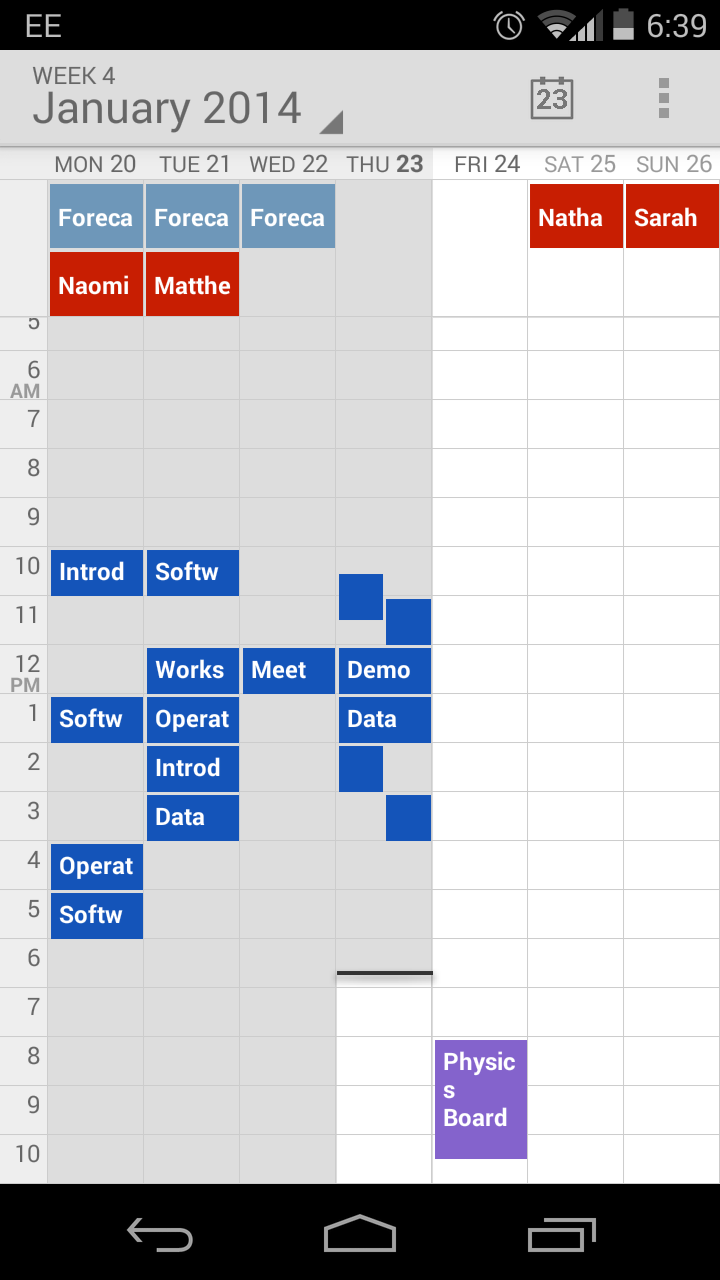
\includegraphics[width=\textwidth]{img/relatedReviews/GoogleCalendarTimetable.png}
		\caption{Google Calendar}\label{fig:GoogleCalendarTimetable}
	\end{subfigure}%
	\qquad
	\begin{subfigure}[b]{0.25\textwidth}
		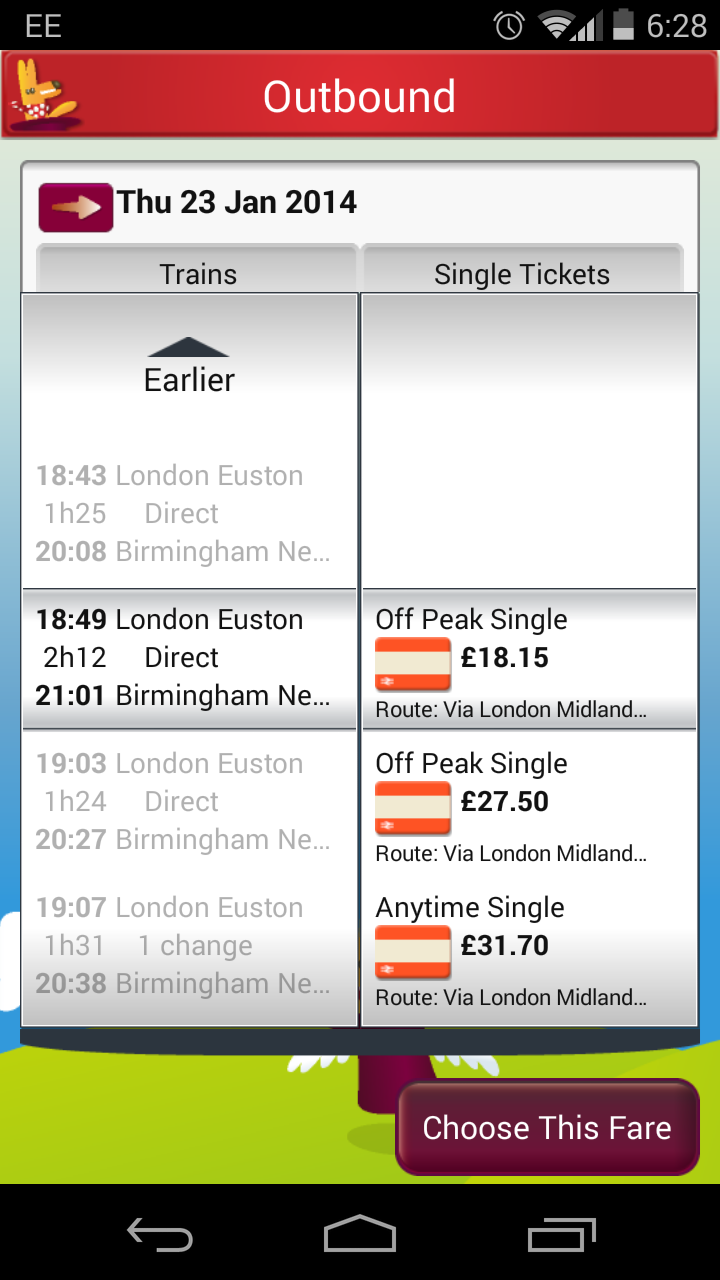
\includegraphics[width=\textwidth]{img/relatedReviews/RedSpottedHankyTicketSelection}
		\caption{RedSpottedHanky}\label{fig:RedSpottedHankyTicketSelection}
	\end{subfigure}
	\caption{When too much information is displayed on a screen, it can be
		hard to read and interpret, whereas condensing the information and
		splitting it so that only currently appropriate information is shown
	makes it much easier to understand. }\label{fig:timetables}
\end{figure}

A common way to improve the readability of theses complex structures, which
often contain a large quantity of data, is to have graded selection of that
data. In other words, where there is an option to refine a search to reduce the
data needed to be displayed, only the  immediately relevant information is
displayed, with simple navigation to other relevant data.

This method can be seen clearly in the RedSpottedHanky.com application,
figure~\ref{fig:RedSpottedHankyTicketSelection} when a user is searching for
tickets for a specific date and time. Although there may be many trains within
a narrow time gap, the application shows a small number of tickets with the
option to move either earlier or later. Each ticket time is also associated
with a number of options relating to ticket price. These are shown only for the
currently selected ticket time.

% subsubsection timetables (end)

\subsubsection{Date/Time Selection}
\label{ssub:date_time_selection}

In order to reduce the search range, often a date and/or time selection
dialogue is used. Figure~\ref{fig:date_time_selection} shows two different
implementations.

Figure~\ref{fig:RedSpottedHankyDateTime}, on the right is an example, again,
from RedSpottedHanky\cite{RedSpottedHanky}, which shows the time selection
associated with booking a train ticket. This design fails since the method of
changing time requires very close control when accuracy is required, and is
time consuming when the desired time is far from the currently selected time.
The movement is performed in single increments or decrements of the hours and
minutes. This is despite the functionality described above which lets the user
view and switch to other trains at nearby times.

Figures~\ref{fig:GoogleCalendarDateTime}, in the middle
and~\ref{fig:GoogleCalendarDateTime2} on the left are examples from Google
Calendar which shows how the process can be made much more intuitive, simple
and fast. Through the use of separate screens with large and clear selection,
this selection is much easier to navigate than the scrolling method used above.
\begin{figure}[ht]
	\centering
	\begin{subfigure}[b]{0.25\textwidth}
		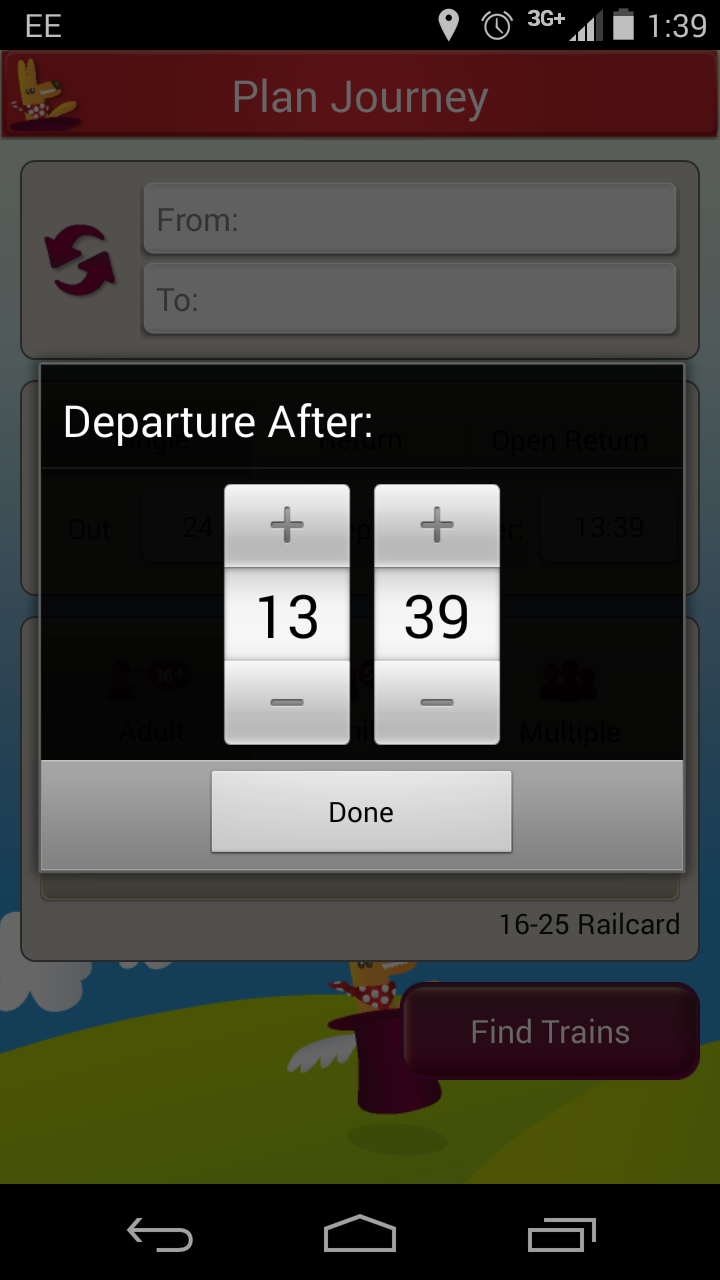
\includegraphics[width=\textwidth]{img/relatedReviews/RedSpottedHankyDateTime}
		\caption{RedSpottedHanky}\label{fig:RedSpottedHankyDateTime}
	\end{subfigure}%
	\qquad
	\begin{subfigure}[b]{0.25\textwidth}
		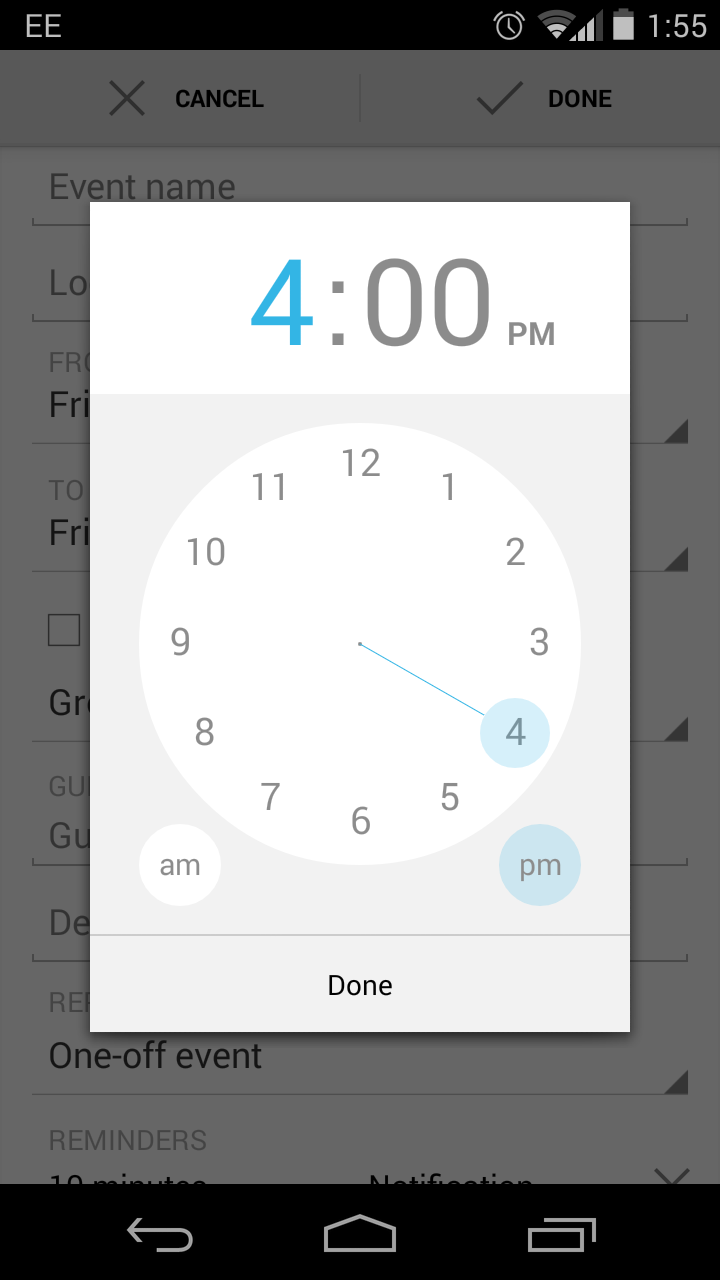
\includegraphics[width=\textwidth]{img/relatedReviews/GoogleCalendarDateTime}
		\caption{Google Calendar}\label{fig:GoogleCalendarDateTime}
	\end{subfigure}
	\qquad
	\begin{subfigure}[b]{0.25\textwidth}
		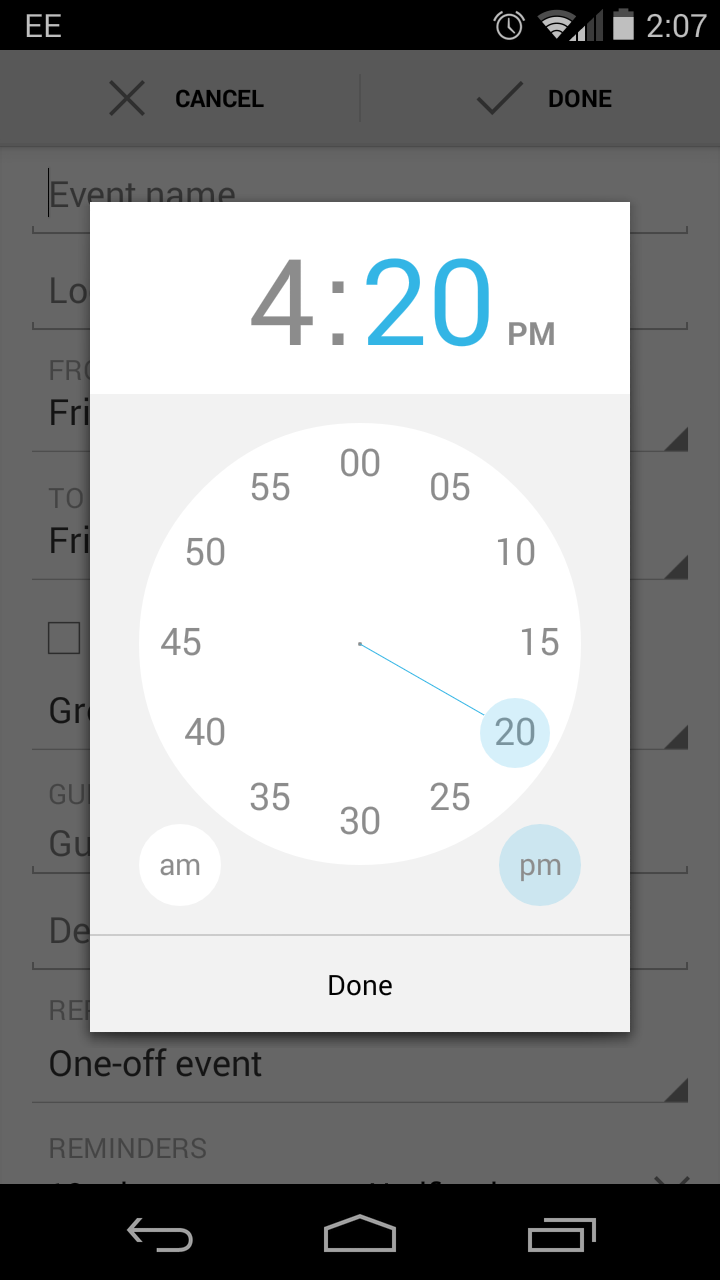
\includegraphics[width=\textwidth]{img/relatedReviews/GoogleCalendarDateTime2}
		\caption{Google Calendar}\label{fig:GoogleCalendarDateTime2}
	\end{subfigure}
	\caption{The time selection for RedSpottedHanky requires the user to
		spend to much time selecting the time when larger increments could be
		used to smoothen the process. Google Calendar, on the other hand,
		allows simple and fast selection of the hours and minutes through
	separate screens. }\label{fig:date_time_selection}
\end{figure}

A combination of both of these is used in the stock iOS, shown in
figure~\ref{fig:iOSDateTime}\cite{iOSDateTime} where a much easier to navigate
scrolling mechanism is used. Though this can still cause the user to spend more
time selecting the correct number, the fact that the used can ``flick scroll''
though the numbers means reaching a value that is far from the currently
selected one is much quicker than the RedSpottedHanky.com application.
\begin{figure}[ht]
	\centering
	\begin{subfigure}[b]{0.25\textwidth}
		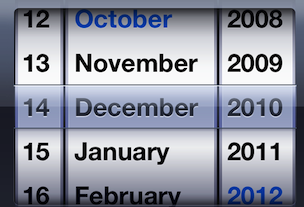
\includegraphics[width=\textwidth]{img/relatedReviews/iOSDateTime}
		\caption{RedSpottedHanky}
	\end{subfigure}%
	\qquad
	\begin{subfigure}[b]{0.35\textwidth}
		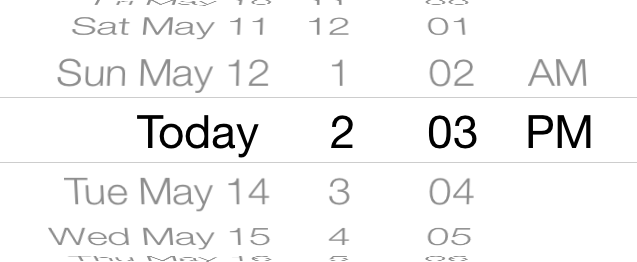
\includegraphics[width=\textwidth]{img/relatedReviews/iOS7DateTime}
		\caption{Google Calendar}
	\end{subfigure}
	\caption{Stock iOS date and time picker is easier to scroll through, but
		still requires more time than selecting the appropriate number.
	}\label{fig:iOSDateTime}
\end{figure}

% subsubsection date_time_selection (end)

\subsubsection{Forms}
\label{ssub:forms}

When entering information that is not limited to a small set of possible
values, such as a name, location or arbitrary number, a form must be used to
accept the user input. Since touch screens rely of the user being able to
navigate to to correct form section, the input must be of sufficient size to
allow this movement easily.

Figure~\ref{fig:TescoFormInput} show a simple form with two input boxes. Each
has a clear border around it so the target for interaction is easier to select.

An important consideration that has been made here is to specify that, for the
second set of text input, the data is strictly limited to digits. For this
reason, the keyboard switches from a general purpose ``qwerty'' keyboard to a
purely numerical version. Again, this assists the user, both by indicating that
only the provided digits are acceptable, and making the input of those digits
easier (often the numbers on a touch screen keyboard are only accessible by
switching modes).
\begin{figure}[ht]
	\centering
	\begin{subfigure}[b]{0.2\textwidth}
		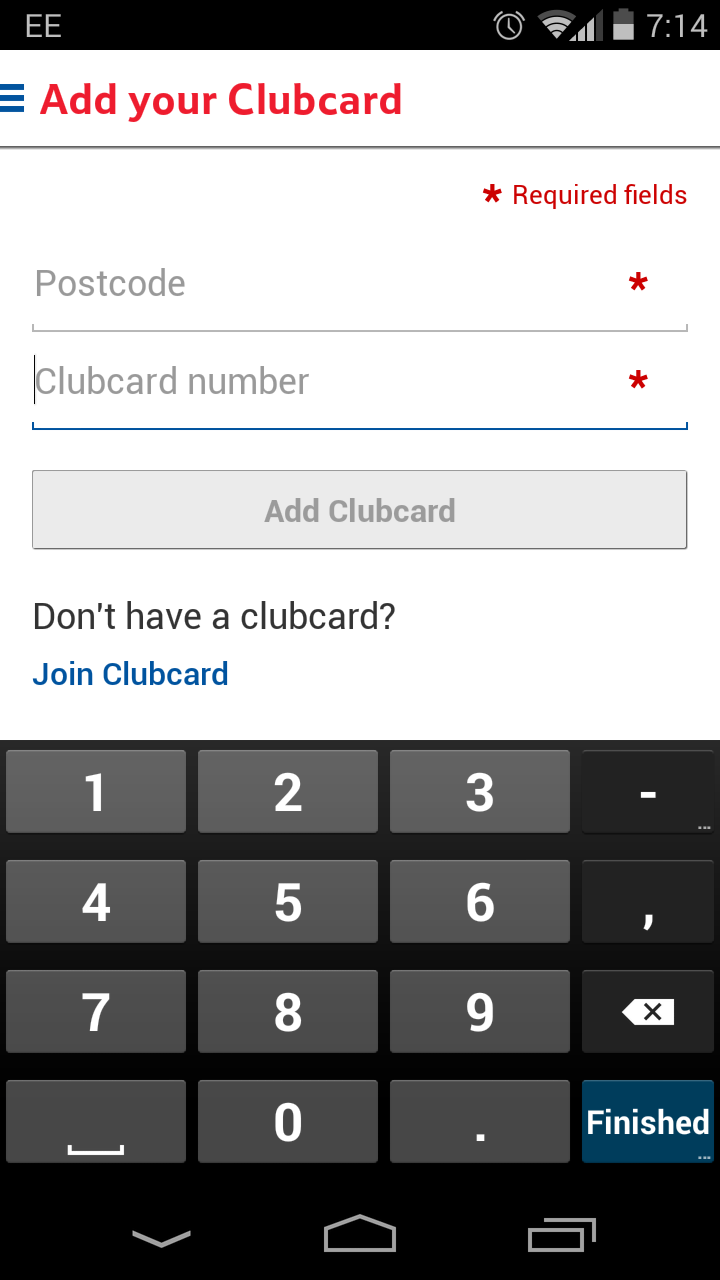
\includegraphics[width=\textwidth]{img/relatedReviews/TescoFormInput}
		\caption{Large, easy to access text entry}\label{fig:TescoFormInput}
	\end{subfigure}%
	\qquad
	\begin{subfigure}[b]{0.25\textwidth}
		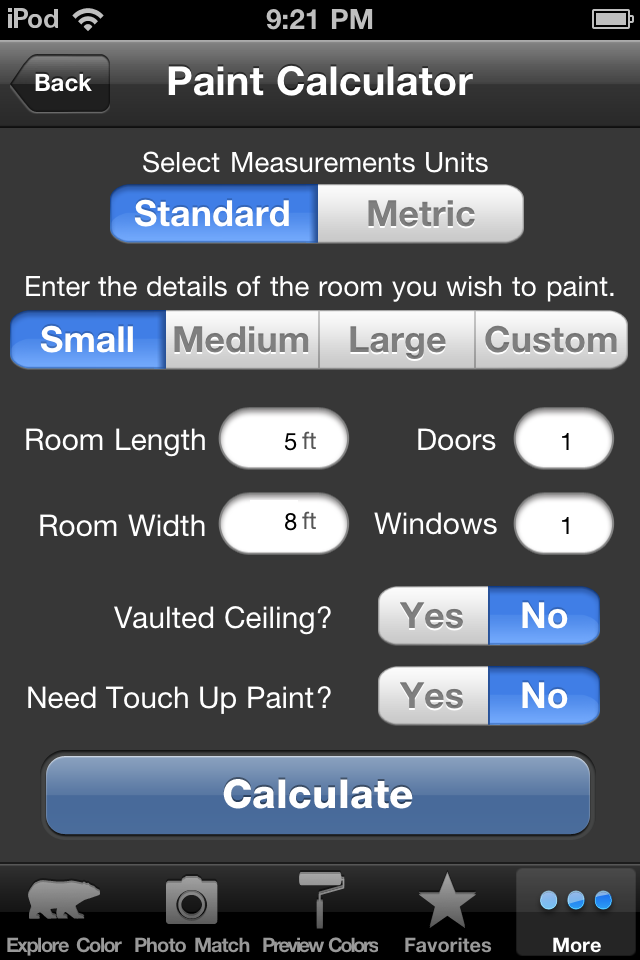
\includegraphics[width=\textwidth]{img/relatedReviews/PaintCalculatorCrowded}
		\caption{Crowded interfaces make entry more difficult.}
	\end{subfigure}
	\caption{}\label{fig:PaintCalculatorCrowded}
\end{figure}

By contrast, the interface in figure~\ref{fig:PaintCalculatorCrowded} is overly
crowded with too many small buttons squashed together. This could cause the
user to select the wrong input area, or not be able to navigate the application
properly.
% subsubsection forms (end)

% subsection user_input (end)

\subsection{Current Comparison/Booking Applications}
\label{sub:current_comparison_applications}

The idea of comparing various services to match your requirements at the best
price is widely spread over the web, especially when it comes to booking
flights, hotels, transport etc.  We want to take this idea and apply it
specifically to booking sports facilities across the county.  Some applications
compare results from different websites; others show available options from
different companies on their own website.

\subsubsection{Skyscanner}
\label{ssub:skyscanner}

Skyscanner is a flight search app which compares flights and airlines. The app
allows the user to search by airport, departure/return date, number of
passengers and cabin class. They are then directed to search results matching
their criteria. Once the user has chosen their desired flight, they are linked
to the airline or travel agent to buy directly.

% \begin{figure}[htbp]
% 	\centering
% 	\begin{subfigure}[b]{0.2\textwidth}
% 		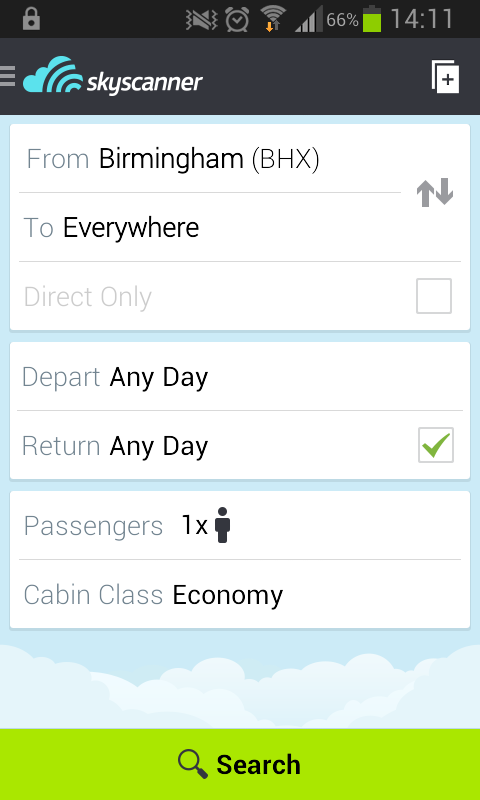
\includegraphics[width=\textwidth]{img/relatedReviews/SkyscannerFig1.png}
% 		\caption{Skyscanner's home screen}\label{fig:skyscannerfig1}
% 	\end{subfigure}%
% 	\qquad
% 	\begin{subfigure}[b]{0.2\textwidth}
% 		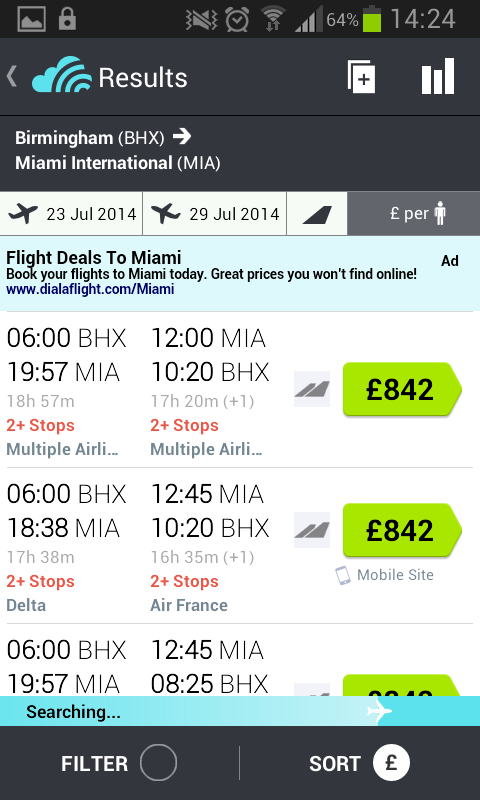
\includegraphics[width=\textwidth]{img/relatedReviews/SkyscannerFig2.png}
% 		\caption{Skyscanner's search results.}
% 	\end{subfigure}
% 	\caption{}\label{fig:skyscanner1}
% \end{figure}

\marginFig[0.8]{img/relatedReviews/SkyscannerFig2.png}{Skyscanner's search results
}{fig:skyscannerfig2}
\paragraph{Strengths}
\begin{itemize}
	\item The date selection page is simplistic and easy to use. The user is
		provided with a calendar where they can simply touch the date they
		would like to fly (figure~\ref{fig:skyscannerfig3}).
	\item Clear, concise information is shown on the results page. This allows
		the user to quickly scan the flights available and doesn't clutter the
		page with information which would not affect most customers' decisions
		(figure~\ref{fig:skyscannerfig2}). Further details (destinations and times
		of any stops) can be viewed by clicking on the flight.
	\item If a return date is not specified, an extra screen is displayed which
		allows the user to see the prices of different departure dates and the
		return dates available. This gives the customer an opportunity to
		change their departure date based on the prices shown.
		(figure~\ref{fig:skyscannerfig5})
	\item There is a filter option on the results page permitting users to be
		more specific. For example, particular airlines, direct flights only,
		flights times etc. (figure~\ref{fig:skyscannerfig4})
\end{itemize}
\begin{figure}[htbp]
	\centering
	\begin{subfigure}[b]{0.28\textwidth}
		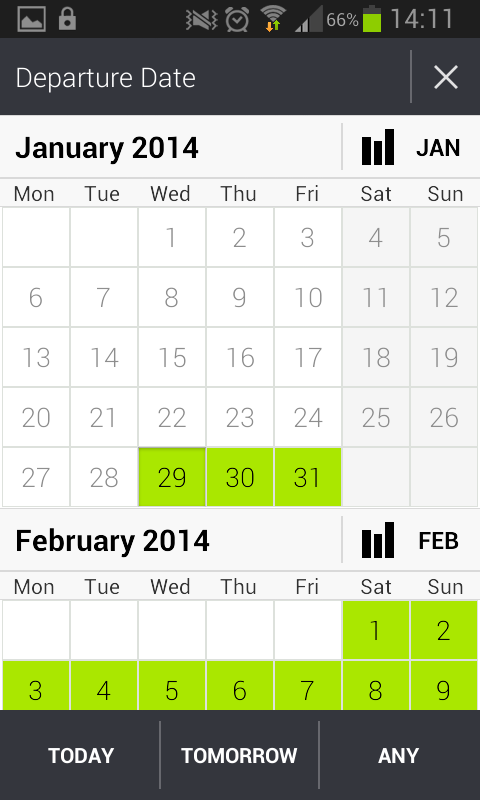
\includegraphics[width=\textwidth]{img/relatedReviews/SkyscannerFig3.png}
		\caption{Skyscanner's easy to use calendar for date selection.
		}\label{fig:skyscannerfig3}
	\end{subfigure}
	\qquad
	\begin{subfigure}[b]{0.28\textwidth}
		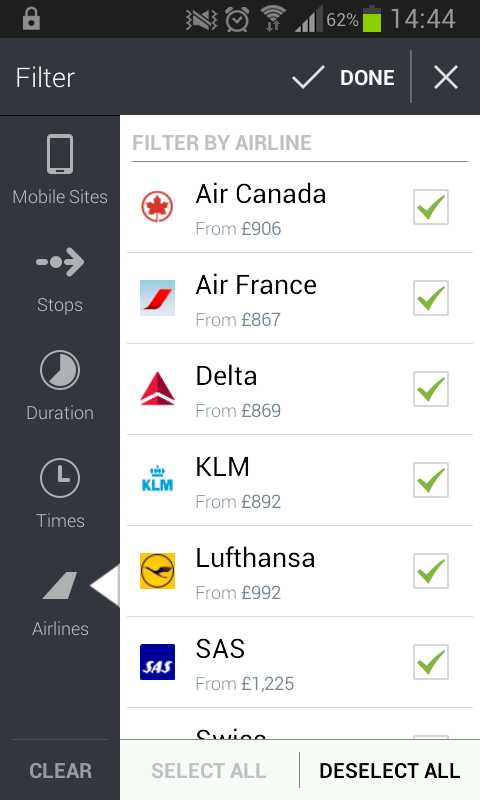
\includegraphics[width=\textwidth]{img/relatedReviews/SkyscannerFig4.png}
		\caption{Options available to further filter search results.
		}\label{fig:skyscannerfig4}
	\end{subfigure}
	\qquad
	\begin{subfigure}[b]{0.28\textwidth}
		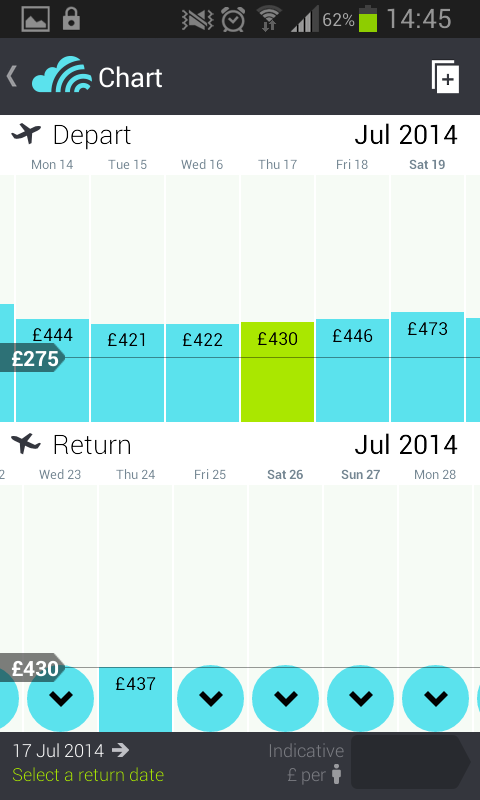
\includegraphics[width=\textwidth]{img/relatedReviews/SkyscannerFig5.png}
		\caption{Screen shows prices of alternative dates.
		}\label{fig:skyscannerfig5}
	\end{subfigure}
	\caption{}\label{fig:skyscanner2}
\end{figure}

\marginFig[0.8]{img/relatedReviews/SkyscannerFig1.png}{Skyscanner's home screen
}{fig:skyscannerfig1}
\paragraph{Weaknesses}
\begin{itemize}
	\item There is no flexibility in departure date (except for the option of
		``any'' date). However the return date option allows flexibility of one
		day.
	\item The ``Everywhere'' option (figure~\ref{fig:skyscannerfig1}) seems
		slightly pointless as it is unlikely someone would have no preference
		as to where they wish to go but have a particular date in mind. It is
		more likely they have a general idea of where they want to go, for
		example the country, but there is no option for this.
	\item When choosing a destination, the user is required to select a
		specific airport. This restricts the user to where they can fly. For
		example, they may wish to check prices to a variety of destinations
		within a particular area or group of Islands with various airports.
\end{itemize}

\subsubsection{Trivago}
\label{ssub:trivago}

Trivago is a hotel comparison website comparing hotels from booking sites such
as booking.com and Lastminute.com. The initial search screen boasts many
options and filters. As well as the expected search criteria such as location
and check in/out date, the user can also filter by rating, popularity,
distance, price and whether the hotel has certain features such as WiFi and a
pool etc. A maximum price and distance can also be set within a certain range
using the sliding bars (figures~\ref{fig:trivago1} and~\ref{fig:trivago1b}).
The results show the cheapest price for each hotel available and what booking
website the customer can get this price. Once the customer has chosen their
hotel, they will be directed to the booking website where they will make the
payment.
\marginFig[0.8]{img/relatedReviews/TrivagoFig1a.png}{Top half}{fig:trivago1}
\marginFig[0.8]{img/relatedReviews/TrivagoFig1b.png}{Bottom half}{fig:trivago1b}
% \begin{figure}[htbp]
% 	\centering
% 	\begin{subfigure}[b]{0.2\textwidth}
% 		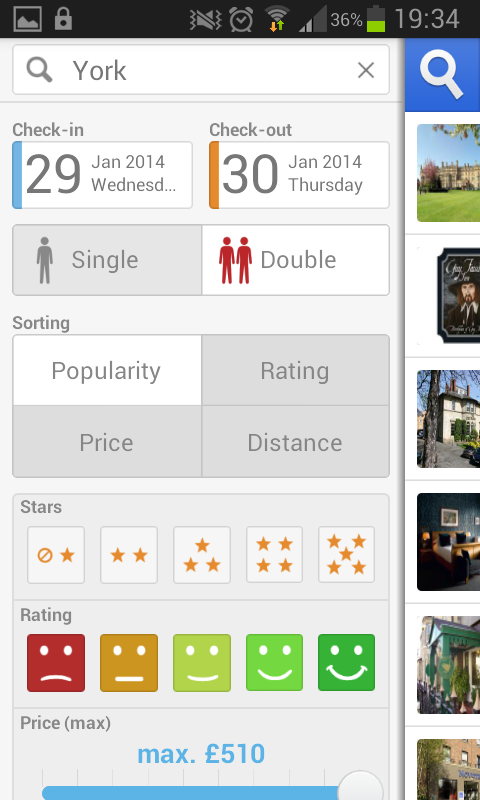
\includegraphics[width=\textwidth]{img/relatedReviews/TrivagoFig1a.png}
% 		\caption{Top half}
% 	\end{subfigure}
% 	\qquad
% 	\begin{subfigure}[b]{0.2\textwidth}
% 		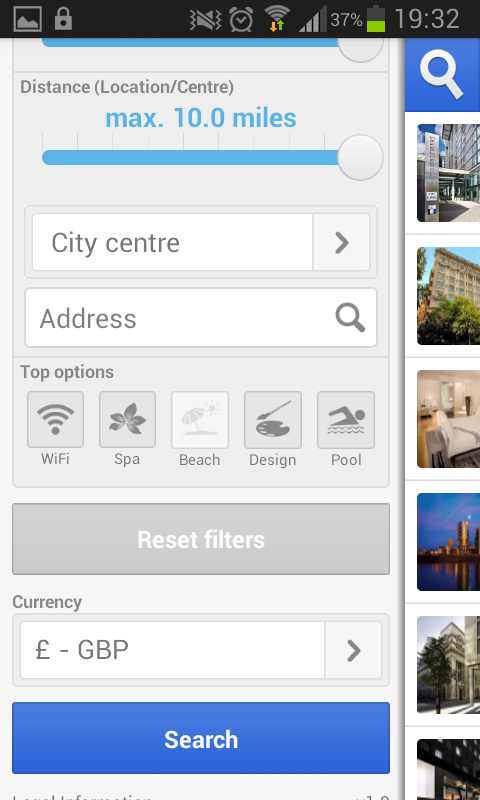
\includegraphics[width=\textwidth]{img/relatedReviews/TrivagoFig1b.png}
% 		\caption{Bottom half}
% 	\end{subfigure}
% 	\caption{Trivago's home screen}\label{fig:trivago1}
% \end{figure}

%TrivagoFig1a.png(home screen top half) TrivagoFig1b.png( home screen bottom half)

\paragraph{Strengths}
\begin{itemize}
	\item As a location is typed, the number of available hotels is displayed
		in brackets next to suggested locations.
	\item Searching is very flexible, for example you can search by hotel name,
		region, points of interest and city.
	\item It is possible to search for hotels in the vicinity of a specific
		address, very useful if you want to find the nearest hotel to a
		specific location.
	\item Search results automatically load up at the side of the screen as
		search criteria is filled out. The user can swipe across to see them,
		for example once a location had been entered, it will load up available
		hotels whilst still maintaining the search screen.
	\item The search results are very clear and simple in that they show enough
		information without clogging up the screen. The hotel name, rating,
		stars, distance from the centre, price and a photo are all displayed in
		a concise manner (figure~\ref{fig:TrivagoFig2}). The user can then look
		into more detail by clicking on the hotel
		(figure~\ref{fig:TrivagoFig3}).
\end{itemize}
\begin{figure}[htbp]
	\centering
	\begin{subfigure}[b]{0.33\textwidth}
		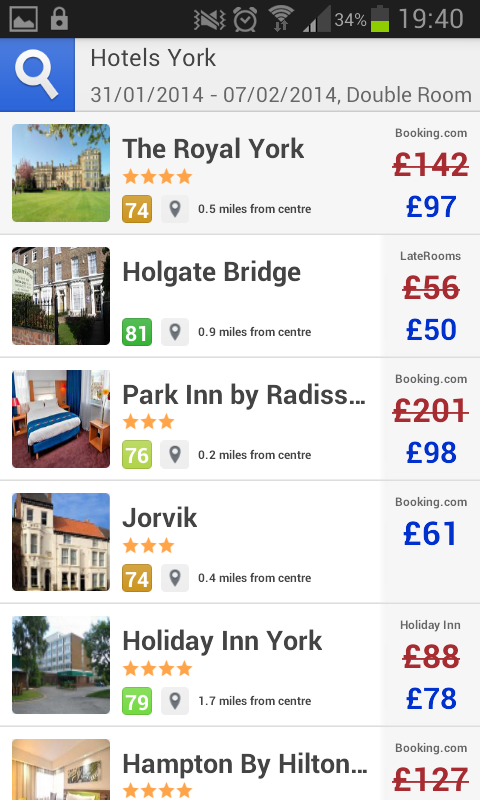
\includegraphics[width=\textwidth]{img/relatedReviews/TrivagoFig2.png}
		\caption{Trivago's earch results screen}\label{fig:TrivagoFig2}
	\end{subfigure}%
	\qquad
	\begin{subfigure}[b]{0.33\textwidth}
		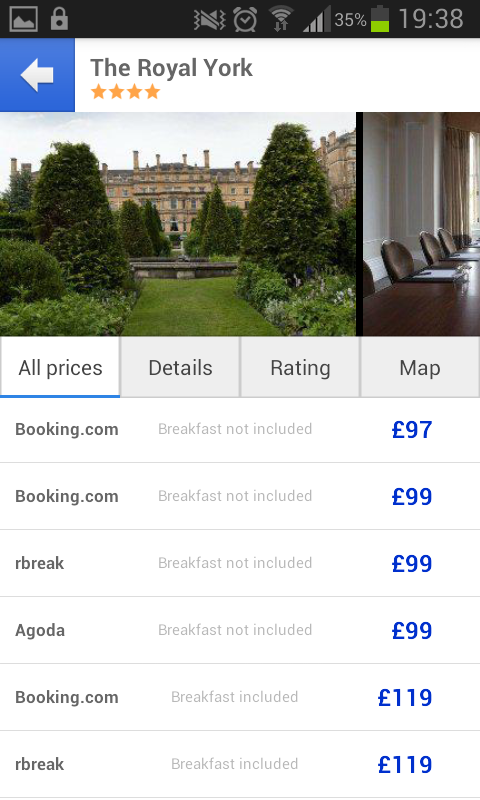
\includegraphics[width=\textwidth]{img/relatedReviews/TrivagoFig3.png}
		\caption{The hotel in more detail}\label{fig:TrivagoFig3}
	\end{subfigure}
	\caption{}\label{fig:trivago2}
\end{figure}

\paragraph{Weaknesses}

\begin{itemize}
	\item The `current location' feature in the search box is useful if you
		need a hotel there and then, but in reality this is rarely the case.
		Customers would usually book a hotel at least a day in advance at which
		point there current location is unlikely to be near an area they would
		need a hotel.
	\item There is no option to select how many people and therefore no option
		for multiple rooms. The user may require multiple rooms if there is
		more than two of them. Therefore this app is useless for families and
		people travelling in large groups.
	\item There are no additional filters past the home screen. Customers may
		require extra filters such as free parking.
\end{itemize}

\subsubsection{thetrainline.com}
\label{ssub:thetrainline}

thetrainline.com is a train ticket retailer app designed to let customers buy
train tickets without the need to have a paper ticket. This app differs
slightly in that it independently searches individual trains without searching
external websites. Train journeys can be searched by location of departure and
destination, departure/arrival  time and number of passengers, as shown in
figure~\ref{fig:theTrainLineFig1}. All available train journeys are then
displayed with the cheapest price for each journey.  Once the customer has
confirmed their chosen journey they can pay for their ticket on
thetrainline.com. The customer will be sent a barcode ticket to their mobile
phone.
% \begin{figure}[htbp]
% 	\centering
% 	\begin{subfigure}[b]{0.2\textwidth}
% 		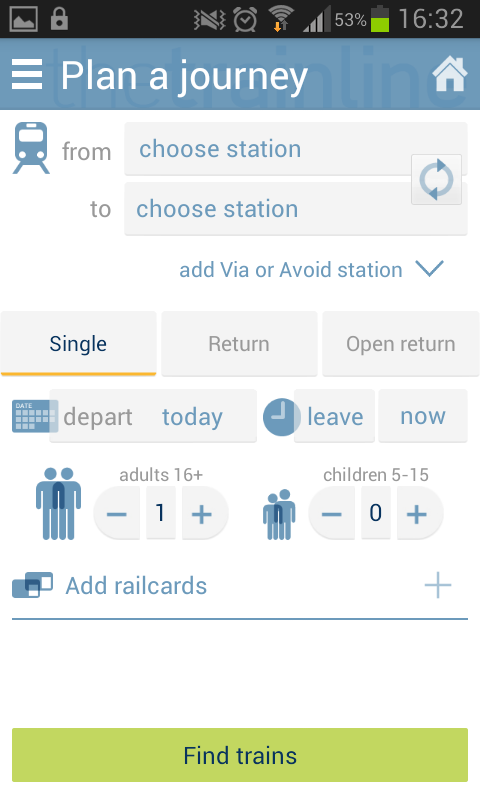
\includegraphics[width=\textwidth]{img/relatedReviews/theTrainLineFig1.png}
% 		\caption{Search criteria screen}\label{fig:theTrainLineFig1}
% 	\end{subfigure}%
% 	\qquad
% 	\begin{subfigure}[b]{0.2\textwidth}
% 		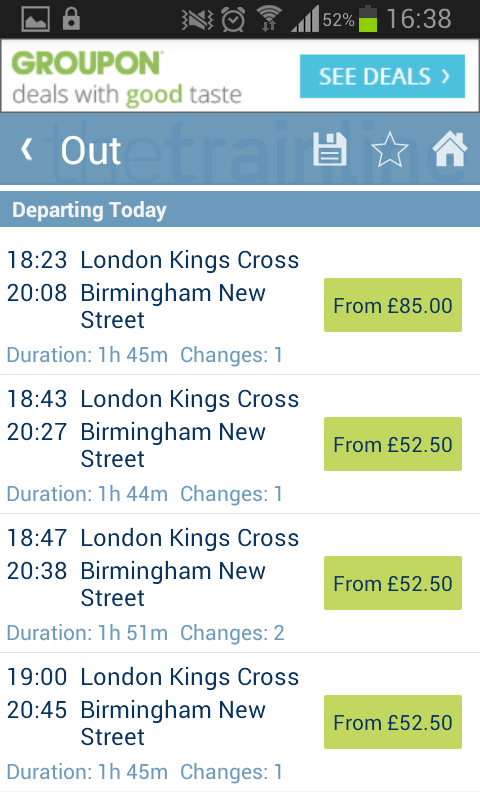
\includegraphics[width=\textwidth]{img/relatedReviews/theTrainLineFig2.png}
% 		\caption{Results from the search}\label{fig:theTrainLineFig2}
% 	\end{subfigure}
% 	\caption{Search using thetrainline.com application.
% 	}\label{fig:thetrainline1}
% \end{figure}
\marginFig[0.8]{img/relatedReviews/theTrainLineFig1.png}{thetrainline search criteria screen}{fig:theTrainLineFig1}
\marginFig[0.8]{img/relatedReviews/theTrainLineFig2.png}{Search results from thetrainline}{fig:theTrainLineFig2}

\paragraph{Strengths}

\begin{itemize}
	\item When typing the name of the station it suggests possible stations
		based on the first few letters. Useful if you're unsure of the name of
		the station. For example, typing `Birmingham' shows a list of all
		stations in Birmingham. In addition to this all recent searches are
		also displayed, so it is not necessary to type the name of the station
		each time.
	\item The app uses GPS to find the customers nearest station and it is also
		possible to set a home station to make it quicker and easier to plan a
		journey home every day (figure~\ref{fig:thetrainline3}).
	\item There is no redirection to another website, the customer can pay
		directly on thetrainline.com which provides a quicker and smoother
		payment process.
	\item The results shown are not limited to the specific time chosen,
		figure~\ref{fig:theTrainLineFig2}. This gives the customer an
		opportunity to choose an earlier or later train if it happens to be a
		lot cheaper.
\end{itemize}
\begin{figure}[htbp]
	\centering
	\begin{subfigure}[b]{0.33\textwidth}
		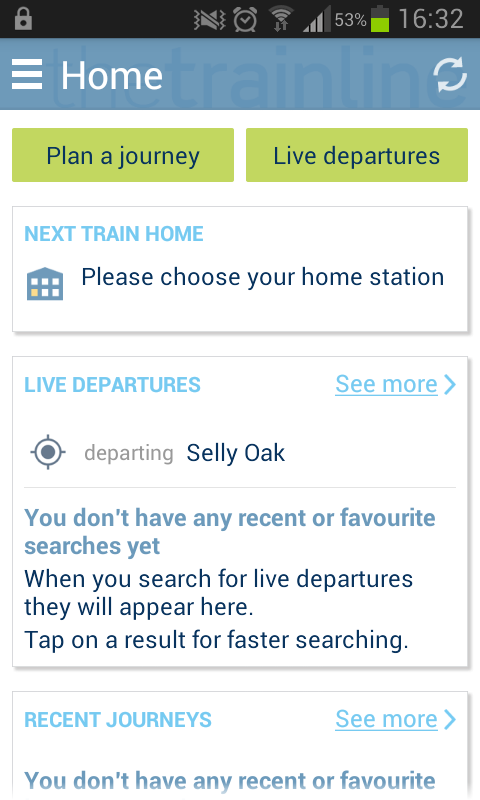
\includegraphics[width=\textwidth]{img/relatedReviews/theTrainLineFig3.png}
		\caption{Home screen showing GPS feature}
	\end{subfigure}%
	\qquad
	\begin{subfigure}[b]{0.33\textwidth}
		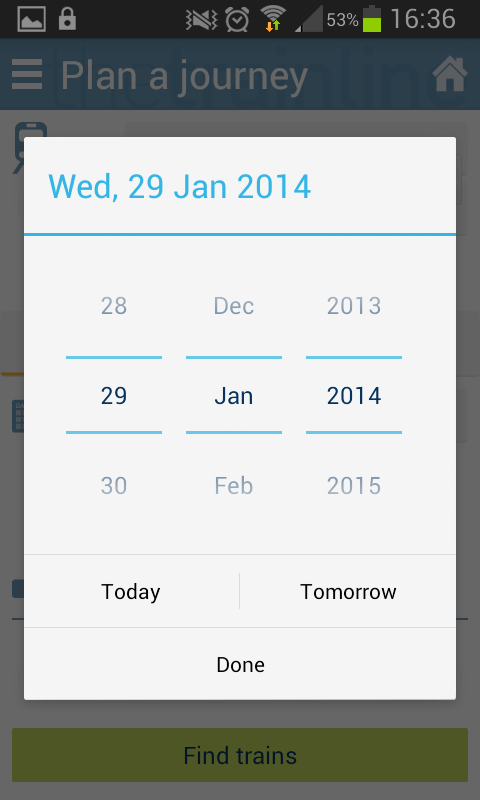
\includegraphics[width=\textwidth]{img/relatedReviews/theTrainLineFig4a.png}
		\caption{Sensitive time selection feature}
	\end{subfigure}
	\caption{}\label{fig:thetrainline3}
\end{figure}

\paragraph{Weaknesses}
\begin{itemize}
	\item The time and date selection feature is very sensitive and therefore
		requires a steady hand when scrolling up and down. The time can also be
		selected to the nearest minute, which when it comes to planning a
		journey, isn't particularly necessary considering multiple journeys are
		shown on the results page. Both these flaws contribute to time taken to
		find the desired journey.
\end{itemize}

\subsubsection{What we can learn}
\label{ssub:what_we_can_learn2}

\begin{itemize}
	\item Our sports booking app would benefit from having a GPS feature as
		those looking to play a particular sport would usually prefer to play
		near their current location. For the same reason, when the results are
		displayed, a filter for distance to the sport venue could be beneficial
		to the user.
	\item It would be useful if a message was sent to the users phone to
		confirm the booking. This will allow the user to check the booking
		details they are likely to forget such as court number or price. If the
		user booked the court well in advance, there could also be an option
		for the user to request  a reminder,  say a day before they are due to
		play.
	\item When searching for a particular location, the user should have the
		option to search by either postcode, address, town or city. By entering
		the city, this gives the user flexibility on location. However if the
		user does not wish to travel far, the other options would be more
		constructive. Either way, there is no restriction on how to search for
		a venue.
\end{itemize}

\subsection{Application Considerations}
\label{sub:application_considerations}

Depending on the operating system, each platform has it's own specific
guidelines on how to provide users with a good experience. Key issues include;
page layout, navigation and interaction.
\marginFig{img/relatedReviews/iOS_page}{iOS page layout recommendation}{fig:iOS_page}

Apple recommends that the most important feature of an app should be displayed
at the top-left of the page so that it will be the first thing a user
sees\cite{HIGApple2013}.  Booking.com and the trainline.com both implement this
well\cite{BookingcomIOS}.
\marginFig[0.7]{img/relatedReviews/booking_page}{Booking page for thetrainline.com\cite{thetrainlineIOS}.}{fig:booking_page}
% \begin{figure}[htbp]
% 	\centering
% 	\begin{subfigure}[b]{0.5\textwidth}
% 		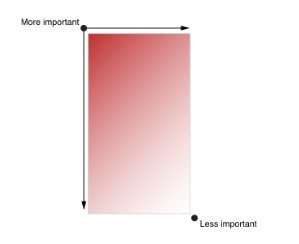
\includegraphics[width=\textwidth]{img/relatedReviews/iOS_page}
% 		\caption{iOS page layout recommendation}\label{fig:iOS_page}
% 	\end{subfigure}%
% 	\qquad
% 	\begin{subfigure}[b]{0.25\textwidth}
% 		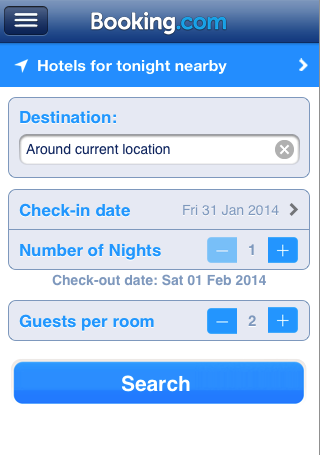
\includegraphics[width=\textwidth]{img/relatedReviews/booking_page}
% 		\caption{Booking page for thetrainline.com\cite{thetrainlineIOS}. }
% 	\end{subfigure}
% 	\caption{}\label{fig:booking_page}
% \end{figure}

Users should be able to navigate their way through the app to achieve their
goal of booking sports facilities.

There are 3 main styles of navigation;
\begin{description}
	\item[Hierarchical] navigation is where users make one choice on the first
		screen, another on the second screen and so on until they reach their
		final destination. To navigate to another destination, the user may
		have to retrace some steps or start over from the beginning. This could
		be very inconvenient for the user as they may have to go back several
		steps or start over.
	\item[Content or Experience-driven] navigation depends on the content of
		the application. The navigation also plays an important part of the app
		experience. The Skyscanner app includes a globe,
		figure~\ref{fig:skyscanner_globe}, which allows the user to explore the
		cost of travelling to particular locations. This is a feature provides
		a unique experience for the user.
		\begin{figure}[htbp]
			\begin{center}
				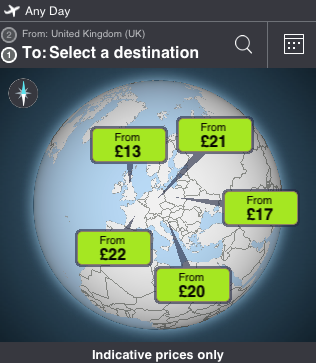
\includegraphics[width=0.4\textwidth]{img/relatedReviews/skyscanner_globe}
			\end{center}
			\caption{Skyscanner apps globe feature}\label{fig:skyscanner_globe}
		\end{figure}

	\item[Flat] navigation allows users are move from one category to another,
		as all categories are available from the main screen. This style has
		been used by many of the apps studied including redspottedhanky.com,
		booking.com and thetrainline.com
		% \begin{figure}[htbp]
		% 	\begin{center}
		% 		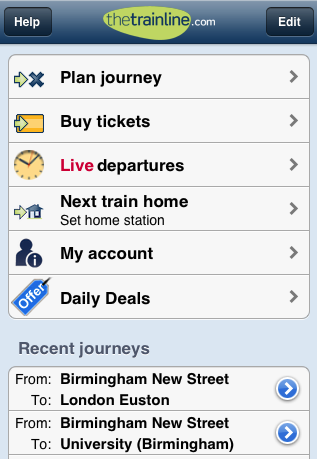
\includegraphics[width=0.25\textwidth]{img/relatedReviews/trainline_main}
		% 	\end{center}
		% 	\caption{Trainline main\cite{thetrainlineIOS}. }\label{fig:trainline_main}
		% \end{figure}
\end{description}

In some cases, it may be better to combine more than one navigation style, but
it could also run the risk of overcomplicating the design of the app and the
user's experience.

Some apps like Trivago have a navigation bar, which manages the screen's
contents. The user can select to change the search criteria or pinpoint hotels
on a map. In the Zipcar app, figure~\ref{fig:zipcar_nav_bar}, the options in
the navigation bar allow the user to perform actions. E.g. `Reserve' or `Log
in'. These options change depending on where the user is in terms of navigation
\begin{figure}[htbp]
	\begin{center}
		
\includegraphics[width=0.45\textwidth]{img/relatedReviews/zipcar_nav_bar1}
		\quad
		
\includegraphics[width=0.45\textwidth]{img/relatedReviews/zipcar_nav_bar2}
	\end{center}
	\caption{Zipcar navigation\cite{ZipCarIOS}.}\label{fig:zipcar_nav_bar}
\end{figure}

Some navigation styles have tab bars placed at the bottom of the screen; this
allows the user to switch between different subtasks, views or modes. For
example, redspottedhanky.com's app includes the options of switching between
finding trains, viewing tickets or account details or finding other
information. This is a useful feature that helps a user navigate their way
through an app, which thetrainline.com has chosen not to use in their design.

Apple and Microsoft both recommend $44\times44$ points and a maximum of 5 icons
to avoid tab bars being over cluttered.
\begin{figure}[htbp]
	\centering
	\begin{subfigure}[b]{0.35\textwidth}
		
\includegraphics[width=\textwidth]{img/relatedReviews/redspottedhanky_tab_bar}
		\caption{RedspottedHanky tab bar. }\label{fig:redspottedhanky_tab_bar}
	\end{subfigure}%
	\qquad
	\begin{subfigure}[b]{0.4\textwidth}
		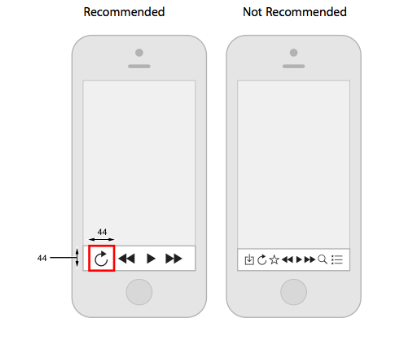
\includegraphics[width=\textwidth]{img/relatedReviews/iOS_tab_bar}
		\caption{iOS tab bar.}\label{fig:iOS_tab_bar}
	\end{subfigure}
	\caption{Tab bar icon sizes.}
\end{figure}

None of the apps studied take into account the orientation of the screen. Users
have no option but to use the apps when the phone is in portrait. It would be
best to provide users with the choice of holding their device in landscape too.
As can be seen in figure~\ref{fig:trivago_input}, Trivago, in particular,
contains a lot of details within its side menu; some users may prefer to see
slightly bigger, which could be possible when the screen is tilted
horizontally.
\marginFig[0.7]{img/relatedReviews/trivago_input}{Trivago input\cite{TrivagoIOS}.}{fig:trivago_input}
% \begin{figure}[htbp]
% 	\begin{center}
% 		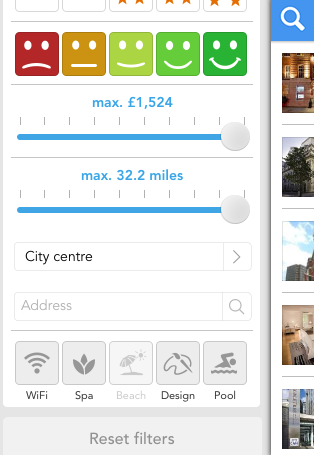
\includegraphics[width=0.25\textwidth]{img/relatedReviews/trivago_input}
% 	\end{center}
% 	\caption{Trivago input\cite{TrivagoIOS}. }\label{fig:trivago_input}
% \end{figure}

The way all of the apps function is through a touchscreen interface. Users may
be used to certain functions such as `pinch to zoom' and other interactions
defined below for iOS\@. It will be important to consider these interactions to
make the app easy to use
\begin{figure}[htbp]
	\centering
	\begin{subfigure}[b]{0.7\textwidth}
		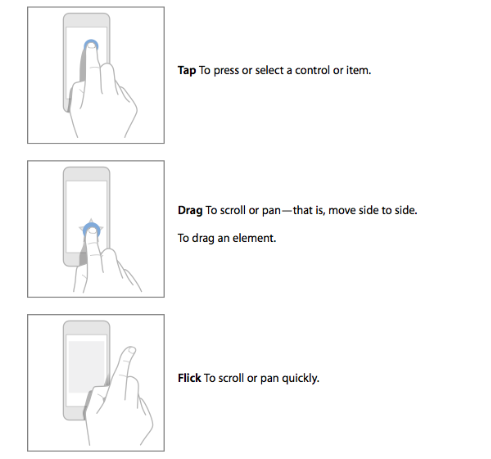
\includegraphics[width=\textwidth]{img/relatedReviews/iOS_touch}
		\caption{iOS touchscreen interactions}\label{fig:iOS_touch}
	\end{subfigure}%
	\qquad
	\begin{subfigure}[b]{0.7\textwidth}
		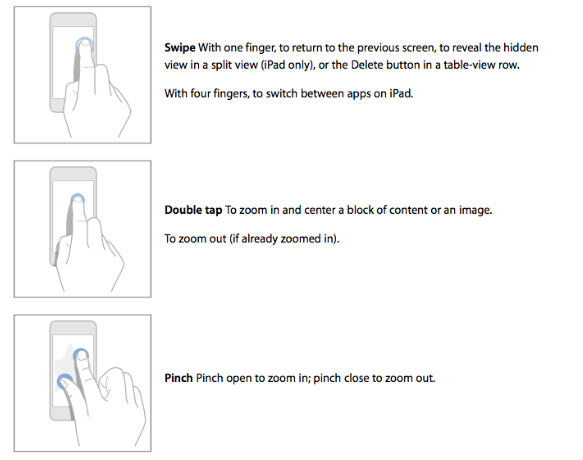
\includegraphics[width=\textwidth]{img/relatedReviews/iOS_touch_2}
		\caption{iOS touchscreen interactions}
	\end{subfigure}
	\caption{}\label{fig:iOS_touch2}
\end{figure}

Other ways the user could provide input include using speech recognition. For
example, the user could say the sport, date, time and location instead of
having to input text or select options.

% subsection application_considerations (end)

\subsection{Current Sports Booking Applications}
\label{sub:current_sports_booking_applications}

Our application will allow searching across multiple organisations, locations,
times and sports to provide available bookings. There are currently no
applications that allow searching across multiple organisations' facilities for
available sports bookings. There are, however, web applications for specific
organisations which:
\begin{itemize}
	\item have multiple locations, each with many available sports to play,
	\item have a single location with many sports to play,
	\item have multiple locations with a single sport to play.
\end{itemize}
There are also web applications which allow for searching of different
facilities but offer no information on available bookings beyond providing
contact information for each facility.

\subsubsection{University Of Birmingham Sport}
\label{ssub:university_of_birmingham_sport}

The University Of Birmingham has an online booking system for numerous sports
available to play at facilities at its campus in Edgbaston\cite{UOBSport}. This
site allows search by location, type of activity and time. Once the user has
entered their search criteria, a list of ``activities'' are returned. The user
then selects an activity and is shown a timetable indicating at what time this
activity is available. The activity can then be booked directly on the website.
\begin{figure}[ht]
	\centering
	\begin{subfigure}[b]{0.4\textwidth}
		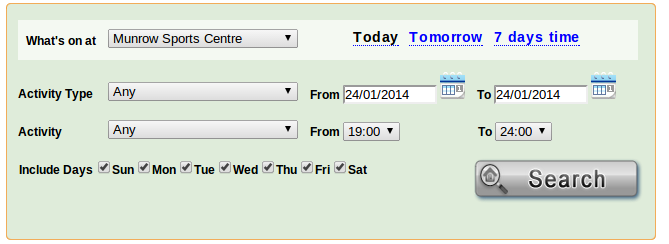
\includegraphics[width=\textwidth]{img/relatedReviews/UoBSearch.png}
		\caption{Search form}\label{fig:UoBSearch}
	\end{subfigure}%
	\qquad
	\begin{subfigure}[b]{0.4\textwidth}
		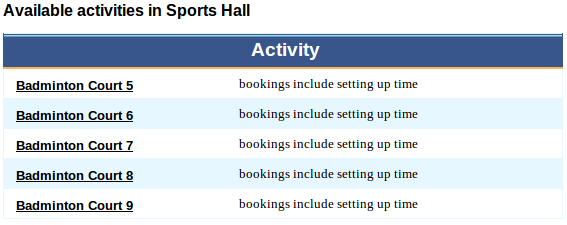
\includegraphics[width=\textwidth]{img/relatedReviews/UoBResults.png}
		\caption{List of results}\label{fig:UoBResults}
	\end{subfigure}
	\qquad
	\begin{subfigure}[b]{0.7\textwidth}
		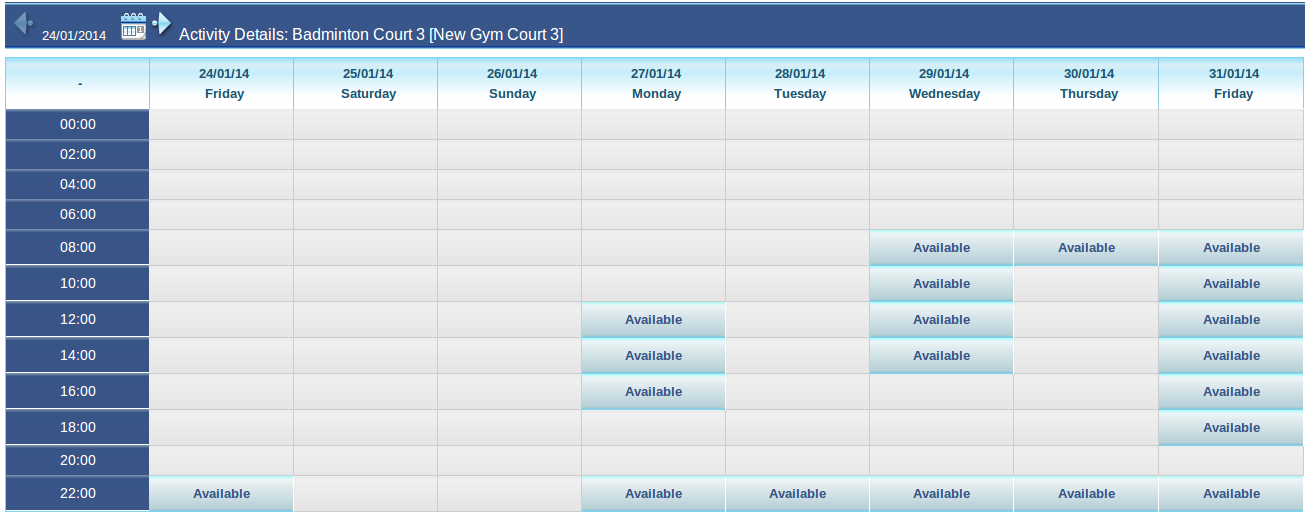
\includegraphics[width=\textwidth]{img/relatedReviews/UoBTimetable.png}
		\caption{Timetable of available bookings}\label{fig:UoBTimetable}
	\end{subfigure}
	\caption{The booking interface for University of Birminghan Sport.
	}\label{fig:animals}
\end{figure}

\paragraph{Strengths}
\begin{itemize}
	\item The search form has tick boxes to filter out particular days of the
		week. A user may only know which days of the week they want to play a
		sport rather than exact dates. This feature gives the user a quick way
		to search for this.
	\item There are quick links on the form to change the date ranges to either
		today, tomorrow or 7 days time. When a group finishes playing a
		particular sport one week, they may want to quickly see what is
		available at the same time the following week; these quick links speed
		up the process of finding these available bookings.
	\item It is possible to search solely by time, leaving all sport and
		location fields blank. If the user knows they want to play a sport at a
		particular time, but would like to have options on sport and location,
		the search form in figure~\ref{fig:UoBSearch} allows them to search
		this way.
\end{itemize}

\paragraph{Weaknesses}
\begin{itemize}
	\item The option to filter by ``activity type'' in the search form is
		actually a filter for location and many of the locations host a variety
		of different sports. Furthermore, the names of these locations, such as
		``Sports Hall'', often offer no clear indication of which sports are
		available at a particular location. If the user wants to know what
		sports are played at a particular venue, they have select that venue
		and then see which options then appear under the ``Activity'' drop down
		box of the search form. This is confusing and unintuitive for the user.
	\item For many sports, such as badminton where there are multiple courts
		available for badminton across several locations, there is no way to
		simply search by that sport. The user is required to go to each court
		individually to see what times are available for that court. The user
		is unlikely to have a court preference and most likely just wants to
		know at what times they can play badminton; this system offers no quick
		and easy way to do this.
	\item The timetable results groups times into two hour slots but often each
		booking slot is one hour long. It will show `available' for a two hour
		slot when at least one of those two hours is available. Therefore it is
		impossible to know if the exact hour a user wants to play is available
		without selecting the containing two hour slot as shown in
		figure~\ref{fig:UoBTimetableDD}.
		\begin{figure}
			\begin{center}
				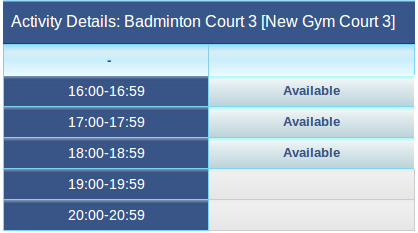
\includegraphics[width=0.4\textwidth]{img/relatedReviews/UoBTimetableDD}
			\end{center}
			\caption{Display when the 18:00 two hour slot is chosen. However,
				only one of two hours following 18:00 is available.
			}\label{fig:UoBTimetableDD}
		\end{figure}

	\item There is no indication of price until you select a booking slot for a
		particular sport at a particular time.
\end{itemize}

\newpage

\subsubsection{Aquaterra Leisure Centres}
\label{ssub:aquaterra_leisure_centres}

Aquaterra is a charity funded by Islington Council who manage several leisure
centres and other sports facilities in Islington, London. They maintain a
website\cite{AquaterraLeisure} where users are able to book at each of these
facilities. The booking home page shown in figure~\ref{fig:AquaterraHome}
prompts a user to select which of the locations they would like to make a
booking at.
\begin{figure}[ht]
	\centering
	\begin{subfigure}[b]{0.3\textwidth}
		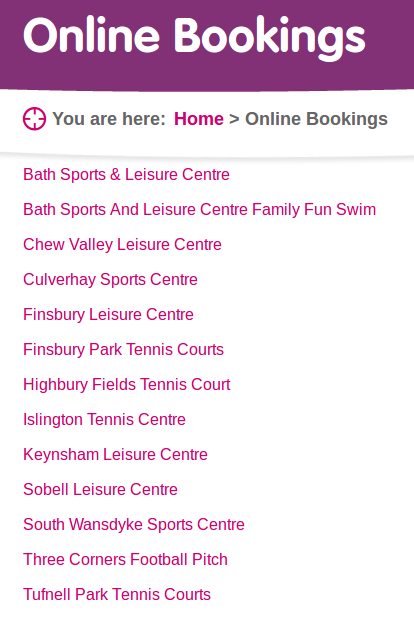
\includegraphics[width=\textwidth]{img/relatedReviews/AquaterraHome.png}
		\caption{Aquaterra booking homepage}\label{fig:AquaterraHome}
	\end{subfigure}
	\qquad
	\begin{subfigure}[b]{0.3\textwidth}
		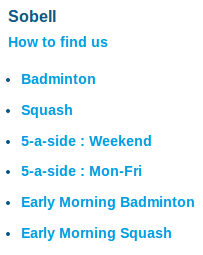
\includegraphics[width=\textwidth]{img/relatedReviews/AquaterraSobellHome.png}
		\caption{Facilities available at Sobell Leisure Centre.
		}\label{fig:AquaterraSobellHome}
	\end{subfigure}
	\qquad
	\caption{The booking interface for Aquaterra Leisure Centres.
	}\label{fig:AquaterraHomeMain}
\end{figure}

The interface for each of the locations varies slightly, but each will
generally show a list of available activities at that location that can be
selected to display a timetable of available booking slots within the following
week for that particular activity. The price is displayed at this point and the
booking can then be made directly on the website after choosing a preferred
court.
\begin{figure}[ht]
	\centering
	\begin{subfigure}[b]{0.4\textwidth}
		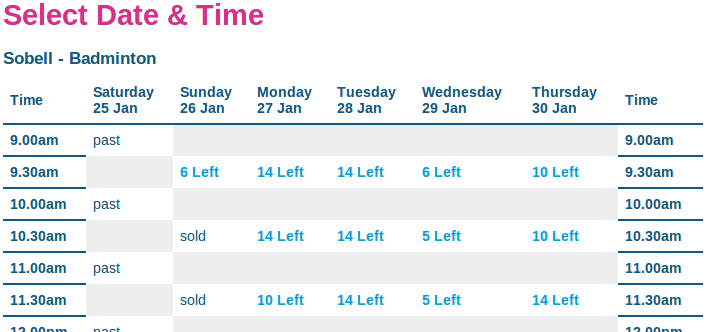
\includegraphics[width=\textwidth]{img/relatedReviews/AquaterraSobellBadminton.png}
		\caption{Beginning of timetable showing available badminton
		slots}\label{fig:AquaterraSobellBadminton}
	\end{subfigure}
	\qquad
	\begin{subfigure}[b]{0.4\textwidth}
		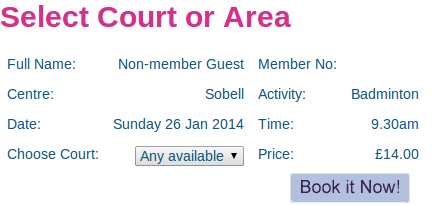
\includegraphics[width=\textwidth]{img/relatedReviews/AquaterraSobellConfirm.png}
		\caption{Confirmation page for a booking slot showing price and choice
		of courts available}\label{fig:AquaterraSobellConfirm}
	\end{subfigure}
	\qquad
	\caption{The booking interface for badminton at Sobell Leisure
	Centre}\label{fig:AquaterraSobellBadmintonMain}
\end{figure}

\paragraph{Strengths}
\begin{itemize}
	\item If a user knows the location they wish to play at and the sport they
		wish to play,  then they can see on one page everything that is
		available to them in the next week. Rows being coloured alternately and
		having the time displayed at both sides of the timetable makes it easy
		for the user to navigate to a particular time slot at a glance.
	\item The timetable for badminton in
		figure~\ref{fig:AquaterraSobellBadminton} indicates how many courts are
		available within each slot. If very few courts are available in a
		preferred time slot, it could indicate to the user that they need to
		make a quick decision as those courts may soon be booked by someone
		else. Conversely, if there are many courts available it could indicate
		to the user that they could delay making a decision on which time to
		book a court. Providing the user with this information early in the
		search process could be very helpful.
\end{itemize}

\paragraph{Weaknesses}
\begin{itemize}
	\item When selecting a location from the page in
		figure~\ref{fig:AquaterraHome}, there is very little indication to the
		user what sports are available at which location. Therefore if they
		want to play a particular sport but have no location preference, they
		are required to go through each option on the homepage to compare what
		facilities are available for that sport at each location. Furthermore,
		as each location's page has a slightly different interface, the user
		has to make sense of each page separately, slowing down their ability
		to compare information provided for each location.
	\item There is no indication of price until you select a particular sport
		at a particular time.
\end{itemize}

\newpage

\subsubsection{London Tennis}
\label{ssub:london_tennis}

London Tennis is a website designed to help tennis players in London find
partners to play with, as well as tournaments to play in and courts to play at.
The court search feature in figure~\ref{fig:LondonTennisSearch} allows a user
to search for a court anywhere in London including options to search by cost of
playing, location and type of court.
\begin{figure}[ht]
	\centering
	\begin{subfigure}[b]{0.6\textwidth}
		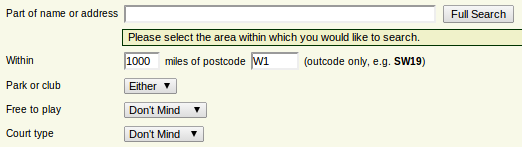
\includegraphics[width=\textwidth]{img/relatedReviews/LondonTennisSearch.png}
		\caption{The search form for looking for a tennis court.
		}\label{fig:LondonTennisSearch}
	\end{subfigure}%
	\qquad
	\begin{subfigure}[b]{0.35\textwidth}
		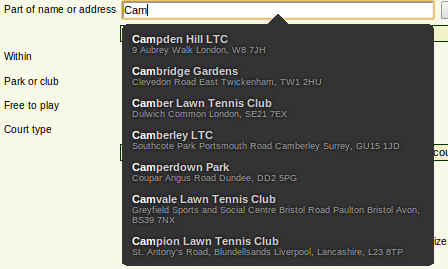
\includegraphics[width=\textwidth]{img/relatedReviews/LondonTennisPredict.png}
		\caption{Drop down to predict input when typing a name of a court.
		}\label{fig:LondonTennisPredict}
	\end{subfigure}
	\qquad
	\caption{The search form for London Tennis.
	}\label{fig:LondonTennisSearchMain}
\end{figure}

There is also the option to select courts from a map, as shown in
figure~\ref{fig:LondonTennisMap}. Users can filter out courts which are free or
not free. However, there are no other interactive features on this map. Once a
search is performed, the user is shown a list of courts matching their chosen
criteria as seen in figure~\ref{fig:LondonTennisResults}. Once a court is
chosen, the user is shown details about the court including exact location,
type of court, price and weather predictions for the local area.
\begin{figure}
	\begin{center}
		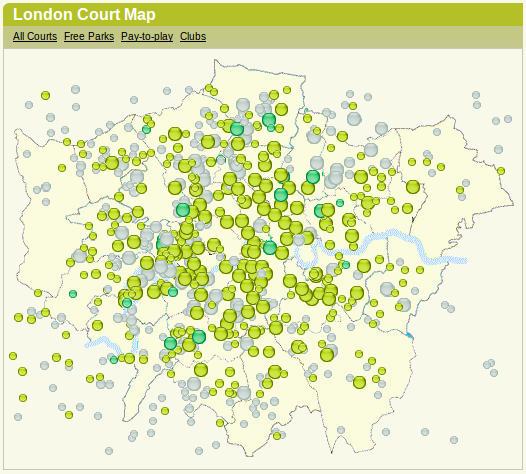
\includegraphics[width=0.7\textwidth]{img/relatedReviews/LondonTennisMap.png}
	\end{center}
	\caption{All courts by location on a map with the ability to filter between
	free and pay-to-play courts}\label{fig:LondonTennisMap}
\end{figure}

\begin{figure}[ht]
	\centering
	\begin{subfigure}[b]{0.7\textwidth}
		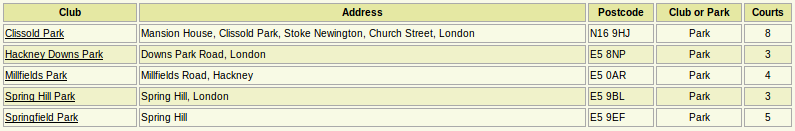
\includegraphics[width=\textwidth]{img/relatedReviews/LondonTennisResults.png}
		\caption{List of courts matching a search.
		}\label{fig:LondonTennisResults}
	\end{subfigure}
	\begin{subfigure}[b]{0.7\textwidth}
		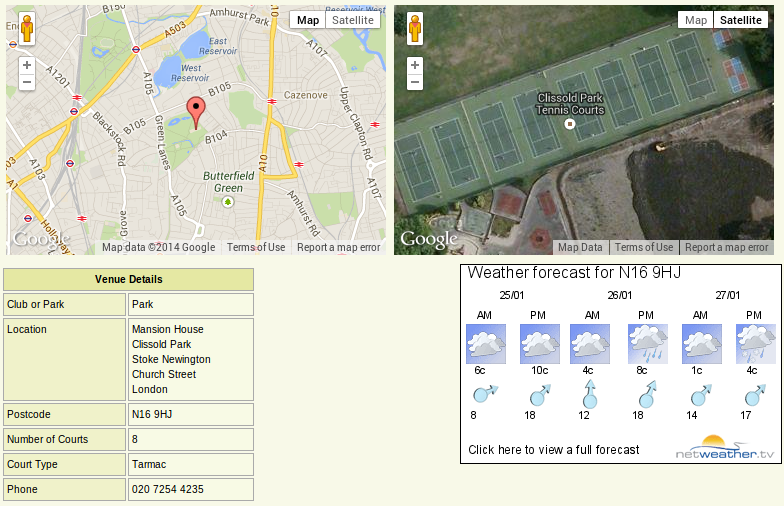
\includegraphics[width=\textwidth]{img/relatedReviews/LondonTennisDetails.png}
		\caption{Details about a chosen court. }\label{fig:LondonTennisDetails}
	\end{subfigure}
	\caption{The displays for results of a search.
	}\label{fig:LondonTennisResultsMain}
\end{figure}

\paragraph{Strengths}
\begin{itemize}
	\item The user is able to show only free courts straight away without
		having to complete any other aspects of the search. This is in contrast
		to other sites we have seen so far and allows the user to immediately
		filter by something that is potentially a deciding factor in choosing a
		court.
	\item The weather predictions are a useful addition given tennis is very
		much dependent on good weather.
\end{itemize}

\paragraph{Weaknesses}
\begin{itemize}
	\item The size of the map for searching in figure~\ref{fig:LondonTennisMap}
		is too small for the number of courts shown on the map, particularly
		given there is no option to zoom in to more detail on the map. Though
		the map does give, at a glance, an idea of where courts are
		concentrated in London, it is difficult to actually select a court due
		to how close the buttons to select each court are to each other.
	\item There is no information about opening times for any of the courts.
		Although London Tennis is primarily a service to find court locations
		rather than provide details about available bookings it would be useful
		to inform the user of when the courts are even open.
\end{itemize}

\subsubsection{What we can learn}
\label{ssub:what_we_can_learn}

\begin{itemize}
	\item It could be useful to add options to filter by day of the week in
		addition to buttons that quickly allow searching by times relative to
		today such as tomorrow or one week from now as this is possibly be one
		of the main criterias of the users search.
	\item The naming of options to filter by when searching need to be
		intuitive and unambiguous otherwise it is difficult  for the user to
		know how to actually search for what they want.
	\item Using a timetable layout similar to figure~\ref{fig:UoBTimetable}
		could create difficulties in clearly displaying all available options
		after a search is done. There may be far more booking slots to display
		in our app given that our search will be conducted over a greater
		number of facilities. The screen space available will also be smaller
		than University of Birmingham has on their website. Therefore we need
		to think of a clearer way of showing the user the results of a search.
	\item Price is likely to be a factor in a user's decision of what sport to
		play and where, therefore our application needs to either provide a
		filter to search by price or clearly indicate the price of a booking
		option as early as possible when displaying results to a user.
	\item If we are to use a map to display results of a search, it will be
		difficult given the potentially large number of results to display
		every option individually on the map, particularly if the map covers a
		large area. Therefore it may be better to group options together,
		possibly by colour or different shapes or picture icons, in order to
		make it possible to read and navigate through the results.
	\item Weather could be an important factor when a user knows when they
		would like to play a sport but want to compare what sports are
		available at that time. When a user is looking at search results for
		outdoor bookings, it could be useful to display weather predictions for
		that time, particularly if the search is in the near future as
		predictions are likely to more accurate for the near future.
\end{itemize}


% section review_of_related_work (end)

\newpage

\section{User Personas}
\label{sec:user_personas}

% \begin{figure}[ht]
% 	\begin{center}
% 		
\includegraphics[width=\textwidth]{img/personas/scales.tex}
% 	\end{center}
% 	\caption{}\label{fig:}
% \end{figure}

% %LaTeX with PSTricks extensions
%%Creator: inkscape 0.48.4
%%Please note this file requires PSTricks extensions
\psset{xunit=.5pt,yunit=.5pt,runit=.5pt}
\begin{pspicture}(744.09448242,1052.36218262)
{
\newrgbcolor{curcolor}{0 0 0}
\pscustom[linestyle=none,fillstyle=solid,fillcolor=curcolor]
{
\newpath
\moveto(96.90563965,916.33235168)
\lineto(97.96813965,916.33235168)
\lineto(100.55407715,911.45344543)
\lineto(100.55407715,916.33235168)
\lineto(101.31970215,916.33235168)
\lineto(101.31970215,910.50032043)
\lineto(100.25720215,910.50032043)
\lineto(97.67126465,915.37922668)
\lineto(97.67126465,910.50032043)
\lineto(96.90563965,910.50032043)
\lineto(96.90563965,916.33235168)
}
}
{
\newrgbcolor{curcolor}{0 0 0}
\pscustom[linestyle=none,fillstyle=solid,fillcolor=curcolor]
{
\newpath
\moveto(104.55407715,914.37141418)
\curveto(104.16865842,914.37141031)(103.86397122,914.2203688)(103.64001465,913.91828918)
\curveto(103.416055,913.6188069)(103.30407595,913.20734898)(103.30407715,912.68391418)
\curveto(103.30407595,912.16047502)(103.41475292,911.74771502)(103.6361084,911.44563293)
\curveto(103.86006498,911.14615312)(104.16605425,910.99641369)(104.55407715,910.99641418)
\curveto(104.93688682,910.99641369)(105.24027193,911.1474552)(105.4642334,911.44953918)
\curveto(105.68818815,911.75162127)(105.8001672,912.16307919)(105.8001709,912.68391418)
\curveto(105.8001672,913.20214065)(105.68818815,913.61229649)(105.4642334,913.91438293)
\curveto(105.24027193,914.21906672)(104.93688682,914.37141031)(104.55407715,914.37141418)
\moveto(104.55407715,914.98078918)
\curveto(105.17907407,914.9807847)(105.669959,914.77765991)(106.0267334,914.37141418)
\curveto(106.38349995,913.96516072)(106.56188519,913.40266128)(106.56188965,912.68391418)
\curveto(106.56188519,911.96776688)(106.38349995,911.40526745)(106.0267334,910.99641418)
\curveto(105.669959,910.59016409)(105.17907407,910.3870393)(104.55407715,910.38703918)
\curveto(103.92647116,910.3870393)(103.43428415,910.59016409)(103.07751465,910.99641418)
\curveto(102.72334736,911.40526745)(102.54626421,911.96776688)(102.54626465,912.68391418)
\curveto(102.54626421,913.40266128)(102.72334736,913.96516072)(103.07751465,914.37141418)
\curveto(103.43428415,914.77765991)(103.92647116,914.9807847)(104.55407715,914.98078918)
}
}
{
\newrgbcolor{curcolor}{0 0 0}
\pscustom[linestyle=none,fillstyle=solid,fillcolor=curcolor]
{
\newpath
\moveto(108.46032715,916.11750793)
\lineto(108.46032715,914.87532043)
\lineto(109.9407959,914.87532043)
\lineto(109.9407959,914.31672668)
\lineto(108.46032715,914.31672668)
\lineto(108.46032715,911.94172668)
\curveto(108.46032568,911.58495477)(108.50850272,911.35578833)(108.6048584,911.25422668)
\curveto(108.70381502,911.15266353)(108.90303357,911.10188233)(109.20251465,911.10188293)
\lineto(109.9407959,911.10188293)
\lineto(109.9407959,910.50032043)
\lineto(109.20251465,910.50032043)
\curveto(108.6478255,910.50032043)(108.26501338,910.60318492)(108.05407715,910.80891418)
\curveto(107.8431388,911.017247)(107.73767016,911.39485079)(107.7376709,911.94172668)
\lineto(107.7376709,914.31672668)
\lineto(107.21032715,914.31672668)
\lineto(107.21032715,914.87532043)
\lineto(107.7376709,914.87532043)
\lineto(107.7376709,916.11750793)
\lineto(108.46032715,916.11750793)
}
}
{
\newrgbcolor{curcolor}{0 0 0}
\pscustom[linestyle=none,fillstyle=solid,fillcolor=curcolor]
{
}
}
{
\newrgbcolor{curcolor}{0 0 0}
\pscustom[linestyle=none,fillstyle=solid,fillcolor=curcolor]
{
\newpath
\moveto(113.46813965,916.33235168)
\lineto(114.25720215,916.33235168)
\lineto(114.25720215,910.50032043)
\lineto(113.46813965,910.50032043)
\lineto(113.46813965,916.33235168)
}
}
{
\newrgbcolor{curcolor}{0 0 0}
\pscustom[linestyle=none,fillstyle=solid,fillcolor=curcolor]
{
\newpath
\moveto(119.20251465,914.03547668)
\curveto(119.38219781,914.35838949)(119.59704134,914.5966705)(119.8470459,914.75032043)
\curveto(120.09704084,914.90396186)(120.39131138,914.9807847)(120.7298584,914.98078918)
\curveto(121.18558142,914.9807847)(121.53714357,914.82062861)(121.7845459,914.50032043)
\curveto(122.03193474,914.18260842)(122.15563254,913.72948387)(122.15563965,913.14094543)
\lineto(122.15563965,910.50032043)
\lineto(121.4329834,910.50032043)
\lineto(121.4329834,913.11750793)
\curveto(121.43297701,913.53677573)(121.35875833,913.84797334)(121.21032715,914.05110168)
\curveto(121.06188363,914.25422293)(120.83532136,914.35578533)(120.53063965,914.35578918)
\curveto(120.1582387,914.35578533)(119.86396816,914.23208754)(119.64782715,913.98469543)
\curveto(119.43167693,913.73729636)(119.32360412,913.40005712)(119.3236084,912.97297668)
\lineto(119.3236084,910.50032043)
\lineto(118.60095215,910.50032043)
\lineto(118.60095215,913.11750793)
\curveto(118.60094859,913.5393799)(118.52672991,913.8505775)(118.3782959,914.05110168)
\curveto(118.22985521,914.25422293)(118.00068877,914.35578533)(117.6907959,914.35578918)
\curveto(117.32360612,914.35578533)(117.03193974,914.23078545)(116.8157959,913.98078918)
\curveto(116.59964851,913.73339012)(116.4915757,913.39745295)(116.49157715,912.97297668)
\lineto(116.49157715,910.50032043)
\lineto(115.7689209,910.50032043)
\lineto(115.7689209,914.87532043)
\lineto(116.49157715,914.87532043)
\lineto(116.49157715,914.19563293)
\curveto(116.65563804,914.46385814)(116.85225242,914.66177461)(117.0814209,914.78938293)
\curveto(117.3105853,914.91698268)(117.58272044,914.9807847)(117.89782715,914.98078918)
\curveto(118.21553231,914.9807847)(118.48506329,914.90005562)(118.7064209,914.73860168)
\curveto(118.93037534,914.57713927)(119.09573976,914.34276451)(119.20251465,914.03547668)
}
}
{
\newrgbcolor{curcolor}{0 0 0}
\pscustom[linestyle=none,fillstyle=solid,fillcolor=curcolor]
{
\newpath
\moveto(124.28845215,911.15657043)
\lineto(124.28845215,908.83625793)
\lineto(123.5657959,908.83625793)
\lineto(123.5657959,914.87532043)
\lineto(124.28845215,914.87532043)
\lineto(124.28845215,914.21125793)
\curveto(124.43949221,914.47167063)(124.62959619,914.66437877)(124.85876465,914.78938293)
\curveto(125.09053323,914.91698268)(125.36657462,914.9807847)(125.68688965,914.98078918)
\curveto(126.21813627,914.9807847)(126.64912542,914.76984742)(126.9798584,914.34797668)
\curveto(127.31318726,913.92609826)(127.47985376,913.37141131)(127.4798584,912.68391418)
\curveto(127.47985376,911.99641269)(127.31318726,911.44172574)(126.9798584,911.01985168)
\curveto(126.64912542,910.59797659)(126.21813627,910.3870393)(125.68688965,910.38703918)
\curveto(125.36657462,910.3870393)(125.09053323,910.44953924)(124.85876465,910.57453918)
\curveto(124.62959619,910.70214315)(124.43949221,910.89615337)(124.28845215,911.15657043)
\moveto(126.73376465,912.68391418)
\curveto(126.73376075,913.21255731)(126.62438586,913.62661939)(126.40563965,913.92610168)
\curveto(126.18949046,914.22818129)(125.89131368,914.37922281)(125.5111084,914.37922668)
\curveto(125.13089777,914.37922281)(124.83141891,914.22818129)(124.6126709,913.92610168)
\curveto(124.39652351,913.62661939)(124.2884507,913.21255731)(124.28845215,912.68391418)
\curveto(124.2884507,912.1552667)(124.39652351,911.73990253)(124.6126709,911.43782043)
\curveto(124.83141891,911.13834063)(125.13089777,910.9886012)(125.5111084,910.98860168)
\curveto(125.89131368,910.9886012)(126.18949046,911.13834063)(126.40563965,911.43782043)
\curveto(126.62438586,911.73990253)(126.73376075,912.1552667)(126.73376465,912.68391418)
}
}
{
\newrgbcolor{curcolor}{0 0 0}
\pscustom[linestyle=none,fillstyle=solid,fillcolor=curcolor]
{
\newpath
\moveto(130.36657715,914.37141418)
\curveto(129.98115842,914.37141031)(129.67647122,914.2203688)(129.45251465,913.91828918)
\curveto(129.228555,913.6188069)(129.11657595,913.20734898)(129.11657715,912.68391418)
\curveto(129.11657595,912.16047502)(129.22725292,911.74771502)(129.4486084,911.44563293)
\curveto(129.67256498,911.14615312)(129.97855425,910.99641369)(130.36657715,910.99641418)
\curveto(130.74938682,910.99641369)(131.05277193,911.1474552)(131.2767334,911.44953918)
\curveto(131.50068815,911.75162127)(131.6126672,912.16307919)(131.6126709,912.68391418)
\curveto(131.6126672,913.20214065)(131.50068815,913.61229649)(131.2767334,913.91438293)
\curveto(131.05277193,914.21906672)(130.74938682,914.37141031)(130.36657715,914.37141418)
\moveto(130.36657715,914.98078918)
\curveto(130.99157407,914.9807847)(131.482459,914.77765991)(131.8392334,914.37141418)
\curveto(132.19599995,913.96516072)(132.37438519,913.40266128)(132.37438965,912.68391418)
\curveto(132.37438519,911.96776688)(132.19599995,911.40526745)(131.8392334,910.99641418)
\curveto(131.482459,910.59016409)(130.99157407,910.3870393)(130.36657715,910.38703918)
\curveto(129.73897116,910.3870393)(129.24678415,910.59016409)(128.89001465,910.99641418)
\curveto(128.53584736,911.40526745)(128.35876421,911.96776688)(128.35876465,912.68391418)
\curveto(128.35876421,913.40266128)(128.53584736,913.96516072)(128.89001465,914.37141418)
\curveto(129.24678415,914.77765991)(129.73897116,914.9807847)(130.36657715,914.98078918)
}
}
{
\newrgbcolor{curcolor}{0 0 0}
\pscustom[linestyle=none,fillstyle=solid,fillcolor=curcolor]
{
\newpath
\moveto(136.0970459,914.20344543)
\curveto(136.01631352,914.25031668)(135.92777195,914.28417082)(135.8314209,914.30500793)
\curveto(135.73766797,914.32844161)(135.63350141,914.34016034)(135.5189209,914.34016418)
\curveto(135.11266859,914.34016034)(134.80016891,914.20734798)(134.5814209,913.94172668)
\curveto(134.36527351,913.67870267)(134.2572007,913.2997968)(134.25720215,912.80500793)
\lineto(134.25720215,910.50032043)
\lineto(133.5345459,910.50032043)
\lineto(133.5345459,914.87532043)
\lineto(134.25720215,914.87532043)
\lineto(134.25720215,914.19563293)
\curveto(134.40824221,914.46125397)(134.6048566,914.65786836)(134.8470459,914.78547668)
\curveto(135.08923112,914.9156806)(135.38350166,914.9807847)(135.7298584,914.98078918)
\curveto(135.77933459,914.9807847)(135.83402204,914.97687846)(135.8939209,914.96907043)
\curveto(135.95381359,914.96385764)(136.02021977,914.95474306)(136.09313965,914.94172668)
\lineto(136.0970459,914.20344543)
}
}
{
\newrgbcolor{curcolor}{0 0 0}
\pscustom[linestyle=none,fillstyle=solid,fillcolor=curcolor]
{
\newpath
\moveto(137.56970215,916.11750793)
\lineto(137.56970215,914.87532043)
\lineto(139.0501709,914.87532043)
\lineto(139.0501709,914.31672668)
\lineto(137.56970215,914.31672668)
\lineto(137.56970215,911.94172668)
\curveto(137.56970068,911.58495477)(137.61787772,911.35578833)(137.7142334,911.25422668)
\curveto(137.81319002,911.15266353)(138.01240857,911.10188233)(138.31188965,911.10188293)
\lineto(139.0501709,911.10188293)
\lineto(139.0501709,910.50032043)
\lineto(138.31188965,910.50032043)
\curveto(137.7572005,910.50032043)(137.37438838,910.60318492)(137.16345215,910.80891418)
\curveto(136.9525138,911.017247)(136.84704516,911.39485079)(136.8470459,911.94172668)
\lineto(136.8470459,914.31672668)
\lineto(136.31970215,914.31672668)
\lineto(136.31970215,914.87532043)
\lineto(136.8470459,914.87532043)
\lineto(136.8470459,916.11750793)
\lineto(137.56970215,916.11750793)
}
}
{
\newrgbcolor{curcolor}{0 0 0}
\pscustom[linestyle=none,fillstyle=solid,fillcolor=curcolor]
{
\newpath
\moveto(141.9876709,912.69953918)
\curveto(141.40693957,912.69953699)(141.00459622,912.6331308)(140.78063965,912.50032043)
\curveto(140.55668,912.36750607)(140.44470095,912.14094379)(140.44470215,911.82063293)
\curveto(140.44470095,911.56542354)(140.5280342,911.36229874)(140.69470215,911.21125793)
\curveto(140.86397136,911.06281987)(141.0931378,910.9886012)(141.38220215,910.98860168)
\curveto(141.78063711,910.9886012)(142.09964721,911.12922606)(142.3392334,911.41047668)
\curveto(142.58141756,911.69432966)(142.70251119,912.07063136)(142.70251465,912.53938293)
\lineto(142.70251465,912.69953918)
\lineto(141.9876709,912.69953918)
\moveto(143.42126465,912.99641418)
\lineto(143.42126465,910.50032043)
\lineto(142.70251465,910.50032043)
\lineto(142.70251465,911.16438293)
\curveto(142.53844886,910.89875754)(142.33402198,910.70214315)(142.0892334,910.57453918)
\curveto(141.84443913,910.44953924)(141.54496027,910.3870393)(141.1907959,910.38703918)
\curveto(140.74287773,910.3870393)(140.38610726,910.51203917)(140.1204834,910.76203918)
\curveto(139.85746195,911.01464284)(139.72595167,911.35188208)(139.72595215,911.77375793)
\curveto(139.72595167,912.26594367)(139.890014,912.63703705)(140.21813965,912.88703918)
\curveto(140.54886751,913.13703655)(141.04105452,913.26203642)(141.69470215,913.26203918)
\lineto(142.70251465,913.26203918)
\lineto(142.70251465,913.33235168)
\curveto(142.70251119,913.66307769)(142.5931363,913.91828577)(142.37438965,914.09797668)
\curveto(142.1582409,914.28026457)(141.85355371,914.37141031)(141.46032715,914.37141418)
\curveto(141.21032518,914.37141031)(140.96683584,914.34146243)(140.7298584,914.28157043)
\curveto(140.49287798,914.22167088)(140.26501363,914.13182722)(140.04626465,914.01203918)
\lineto(140.04626465,914.67610168)
\curveto(140.30928442,914.77765991)(140.5644925,914.85318067)(140.81188965,914.90266418)
\curveto(141.05928367,914.95474306)(141.30016884,914.9807847)(141.5345459,914.98078918)
\curveto(142.16735548,914.9807847)(142.64001125,914.81672237)(142.95251465,914.48860168)
\curveto(143.26501063,914.16047302)(143.42126047,913.66307769)(143.42126465,912.99641418)
}
}
{
\newrgbcolor{curcolor}{0 0 0}
\pscustom[linestyle=none,fillstyle=solid,fillcolor=curcolor]
{
\newpath
\moveto(148.5423584,913.14094543)
\lineto(148.5423584,910.50032043)
\lineto(147.8236084,910.50032043)
\lineto(147.8236084,913.11750793)
\curveto(147.82360473,913.5315674)(147.74287564,913.84146293)(147.5814209,914.04719543)
\curveto(147.4199593,914.25292085)(147.17777204,914.35578533)(146.8548584,914.35578918)
\curveto(146.46683525,914.35578533)(146.16084597,914.23208754)(145.93688965,913.98469543)
\curveto(145.71292975,913.73729636)(145.6009507,913.40005712)(145.60095215,912.97297668)
\lineto(145.60095215,910.50032043)
\lineto(144.8782959,910.50032043)
\lineto(144.8782959,914.87532043)
\lineto(145.60095215,914.87532043)
\lineto(145.60095215,914.19563293)
\curveto(145.77282553,914.45864981)(145.97464824,914.6552642)(146.2064209,914.78547668)
\curveto(146.44079361,914.9156806)(146.71032459,914.9807847)(147.01501465,914.98078918)
\curveto(147.51761545,914.9807847)(147.8978234,914.82453486)(148.15563965,914.51203918)
\curveto(148.41344789,914.20213965)(148.54235401,913.74510886)(148.5423584,913.14094543)
}
}
{
\newrgbcolor{curcolor}{0 0 0}
\pscustom[linestyle=none,fillstyle=solid,fillcolor=curcolor]
{
\newpath
\moveto(150.69470215,916.11750793)
\lineto(150.69470215,914.87532043)
\lineto(152.1751709,914.87532043)
\lineto(152.1751709,914.31672668)
\lineto(150.69470215,914.31672668)
\lineto(150.69470215,911.94172668)
\curveto(150.69470068,911.58495477)(150.74287772,911.35578833)(150.8392334,911.25422668)
\curveto(150.93819002,911.15266353)(151.13740857,911.10188233)(151.43688965,911.10188293)
\lineto(152.1751709,911.10188293)
\lineto(152.1751709,910.50032043)
\lineto(151.43688965,910.50032043)
\curveto(150.8822005,910.50032043)(150.49938838,910.60318492)(150.28845215,910.80891418)
\curveto(150.0775138,911.017247)(149.97204516,911.39485079)(149.9720459,911.94172668)
\lineto(149.9720459,914.31672668)
\lineto(149.44470215,914.31672668)
\lineto(149.44470215,914.87532043)
\lineto(149.9720459,914.87532043)
\lineto(149.9720459,916.11750793)
\lineto(150.69470215,916.11750793)
}
}
{
\newrgbcolor{curcolor}{0 0 0}
\pscustom[linestyle=none,fillstyle=solid,fillcolor=curcolor]
{
\newpath
\moveto(297.32998657,910.50032043)
\lineto(295.10342407,916.33235168)
\lineto(295.92764282,916.33235168)
\lineto(297.77529907,911.42219543)
\lineto(299.62686157,916.33235168)
\lineto(300.44717407,916.33235168)
\lineto(298.22451782,910.50032043)
\lineto(297.32998657,910.50032043)
}
}
{
\newrgbcolor{curcolor}{0 0 0}
\pscustom[linestyle=none,fillstyle=solid,fillcolor=curcolor]
{
\newpath
\moveto(304.38076782,912.86750793)
\lineto(304.38076782,912.51594543)
\lineto(301.07608032,912.51594543)
\curveto(301.1073291,912.02115225)(301.25576645,911.64354846)(301.52139282,911.38313293)
\curveto(301.78962008,911.12531981)(302.16201554,910.99641369)(302.63858032,910.99641418)
\curveto(302.91461896,910.99641369)(303.18154578,911.03026782)(303.43936157,911.09797668)
\curveto(303.69977442,911.16568435)(303.95758667,911.26724675)(304.21279907,911.40266418)
\lineto(304.21279907,910.72297668)
\curveto(303.9549825,910.61360157)(303.69065985,910.53026832)(303.41983032,910.47297668)
\curveto(303.14899372,910.4156851)(302.87425442,910.3870393)(302.59561157,910.38703918)
\curveto(301.89769289,910.3870393)(301.34430803,910.59016409)(300.93545532,910.99641418)
\curveto(300.52920468,911.40266328)(300.32607988,911.9521419)(300.32608032,912.64485168)
\curveto(300.32607988,913.36099466)(300.51878802,913.92870242)(300.90420532,914.34797668)
\curveto(301.29222475,914.76984742)(301.81435964,914.9807847)(302.47061157,914.98078918)
\curveto(303.05915006,914.9807847)(303.52399335,914.79068073)(303.86514282,914.41047668)
\curveto(304.2088885,914.03286899)(304.38076333,913.51854658)(304.38076782,912.86750793)
\moveto(303.66201782,913.07844543)
\curveto(303.65680572,913.47167163)(303.54612874,913.7854734)(303.32998657,914.01985168)
\curveto(303.11644167,914.25422293)(302.83258779,914.37141031)(302.47842407,914.37141418)
\curveto(302.07738021,914.37141031)(301.75576595,914.25812918)(301.51358032,914.03157043)
\curveto(301.2739956,913.80500463)(301.1359749,913.48599453)(301.09951782,913.07453918)
\lineto(303.66201782,913.07844543)
}
}
{
\newrgbcolor{curcolor}{0 0 0}
\pscustom[linestyle=none,fillstyle=solid,fillcolor=curcolor]
{
\newpath
\moveto(308.09561157,914.20344543)
\curveto(308.0148792,914.25031668)(307.92633762,914.28417082)(307.82998657,914.30500793)
\curveto(307.73623364,914.32844161)(307.63206708,914.34016034)(307.51748657,914.34016418)
\curveto(307.11123427,914.34016034)(306.79873458,914.20734798)(306.57998657,913.94172668)
\curveto(306.36383918,913.67870267)(306.25576637,913.2997968)(306.25576782,912.80500793)
\lineto(306.25576782,910.50032043)
\lineto(305.53311157,910.50032043)
\lineto(305.53311157,914.87532043)
\lineto(306.25576782,914.87532043)
\lineto(306.25576782,914.19563293)
\curveto(306.40680789,914.46125397)(306.60342228,914.65786836)(306.84561157,914.78547668)
\curveto(307.08779679,914.9156806)(307.38206733,914.9807847)(307.72842407,914.98078918)
\curveto(307.77790027,914.9807847)(307.83258771,914.97687846)(307.89248657,914.96907043)
\curveto(307.95237926,914.96385764)(308.01878544,914.95474306)(308.09170532,914.94172668)
\lineto(308.09561157,914.20344543)
}
}
{
\newrgbcolor{curcolor}{0 0 0}
\pscustom[linestyle=none,fillstyle=solid,fillcolor=curcolor]
{
\newpath
\moveto(310.67764282,910.09407043)
\curveto(310.47451545,909.57323803)(310.27659898,909.23339462)(310.08389282,909.07453918)
\curveto(309.8911827,908.9156866)(309.63337046,908.8362596)(309.31045532,908.83625793)
\lineto(308.73623657,908.83625793)
\lineto(308.73623657,909.43782043)
\lineto(309.15811157,909.43782043)
\curveto(309.35602699,909.4378215)(309.50967267,909.48469645)(309.61904907,909.57844543)
\curveto(309.72842245,909.67219626)(309.84951608,909.89355021)(309.98233032,910.24250793)
\lineto(310.11123657,910.57063293)
\lineto(308.34170532,914.87532043)
\lineto(309.10342407,914.87532043)
\lineto(310.47061157,911.45344543)
\lineto(311.83779907,914.87532043)
\lineto(312.59951782,914.87532043)
\lineto(310.67764282,910.09407043)
}
}
{
\newrgbcolor{curcolor}{0 0 0}
\pscustom[linestyle=none,fillstyle=solid,fillcolor=curcolor]
{
}
}
{
\newrgbcolor{curcolor}{0 0 0}
\pscustom[linestyle=none,fillstyle=solid,fillcolor=curcolor]
{
\newpath
\moveto(316.16983032,916.33235168)
\lineto(316.95889282,916.33235168)
\lineto(316.95889282,910.50032043)
\lineto(316.16983032,910.50032043)
\lineto(316.16983032,916.33235168)
}
}
{
\newrgbcolor{curcolor}{0 0 0}
\pscustom[linestyle=none,fillstyle=solid,fillcolor=curcolor]
{
\newpath
\moveto(321.90420532,914.03547668)
\curveto(322.08388848,914.35838949)(322.29873202,914.5966705)(322.54873657,914.75032043)
\curveto(322.79873152,914.90396186)(323.09300206,914.9807847)(323.43154907,914.98078918)
\curveto(323.8872721,914.9807847)(324.23883424,914.82062861)(324.48623657,914.50032043)
\curveto(324.73362542,914.18260842)(324.85732321,913.72948387)(324.85733032,913.14094543)
\lineto(324.85733032,910.50032043)
\lineto(324.13467407,910.50032043)
\lineto(324.13467407,913.11750793)
\curveto(324.13466768,913.53677573)(324.06044901,913.84797334)(323.91201782,914.05110168)
\curveto(323.7635743,914.25422293)(323.53701203,914.35578533)(323.23233032,914.35578918)
\curveto(322.85992937,914.35578533)(322.56565883,914.23208754)(322.34951782,913.98469543)
\curveto(322.1333676,913.73729636)(322.02529479,913.40005712)(322.02529907,912.97297668)
\lineto(322.02529907,910.50032043)
\lineto(321.30264282,910.50032043)
\lineto(321.30264282,913.11750793)
\curveto(321.30263926,913.5393799)(321.22842059,913.8505775)(321.07998657,914.05110168)
\curveto(320.93154588,914.25422293)(320.70237945,914.35578533)(320.39248657,914.35578918)
\curveto(320.02529679,914.35578533)(319.73363042,914.23078545)(319.51748657,913.98078918)
\curveto(319.30133918,913.73339012)(319.19326637,913.39745295)(319.19326782,912.97297668)
\lineto(319.19326782,910.50032043)
\lineto(318.47061157,910.50032043)
\lineto(318.47061157,914.87532043)
\lineto(319.19326782,914.87532043)
\lineto(319.19326782,914.19563293)
\curveto(319.35732871,914.46385814)(319.5539431,914.66177461)(319.78311157,914.78938293)
\curveto(320.01227597,914.91698268)(320.28441112,914.9807847)(320.59951782,914.98078918)
\curveto(320.91722298,914.9807847)(321.18675396,914.90005562)(321.40811157,914.73860168)
\curveto(321.63206602,914.57713927)(321.79743044,914.34276451)(321.90420532,914.03547668)
}
}
{
\newrgbcolor{curcolor}{0 0 0}
\pscustom[linestyle=none,fillstyle=solid,fillcolor=curcolor]
{
\newpath
\moveto(326.99014282,911.15657043)
\lineto(326.99014282,908.83625793)
\lineto(326.26748657,908.83625793)
\lineto(326.26748657,914.87532043)
\lineto(326.99014282,914.87532043)
\lineto(326.99014282,914.21125793)
\curveto(327.14118289,914.47167063)(327.33128687,914.66437877)(327.56045532,914.78938293)
\curveto(327.7922239,914.91698268)(328.06826529,914.9807847)(328.38858032,914.98078918)
\curveto(328.91982694,914.9807847)(329.3508161,914.76984742)(329.68154907,914.34797668)
\curveto(330.01487793,913.92609826)(330.18154443,913.37141131)(330.18154907,912.68391418)
\curveto(330.18154443,911.99641269)(330.01487793,911.44172574)(329.68154907,911.01985168)
\curveto(329.3508161,910.59797659)(328.91982694,910.3870393)(328.38858032,910.38703918)
\curveto(328.06826529,910.3870393)(327.7922239,910.44953924)(327.56045532,910.57453918)
\curveto(327.33128687,910.70214315)(327.14118289,910.89615337)(326.99014282,911.15657043)
\moveto(329.43545532,912.68391418)
\curveto(329.43545143,913.21255731)(329.32607654,913.62661939)(329.10733032,913.92610168)
\curveto(328.89118114,914.22818129)(328.59300435,914.37922281)(328.21279907,914.37922668)
\curveto(327.83258845,914.37922281)(327.53310958,914.22818129)(327.31436157,913.92610168)
\curveto(327.09821418,913.62661939)(326.99014137,913.21255731)(326.99014282,912.68391418)
\curveto(326.99014137,912.1552667)(327.09821418,911.73990253)(327.31436157,911.43782043)
\curveto(327.53310958,911.13834063)(327.83258845,910.9886012)(328.21279907,910.98860168)
\curveto(328.59300435,910.9886012)(328.89118114,911.13834063)(329.10733032,911.43782043)
\curveto(329.32607654,911.73990253)(329.43545143,912.1552667)(329.43545532,912.68391418)
}
}
{
\newrgbcolor{curcolor}{0 0 0}
\pscustom[linestyle=none,fillstyle=solid,fillcolor=curcolor]
{
\newpath
\moveto(333.06826782,914.37141418)
\curveto(332.68284909,914.37141031)(332.3781619,914.2203688)(332.15420532,913.91828918)
\curveto(331.93024568,913.6188069)(331.81826662,913.20734898)(331.81826782,912.68391418)
\curveto(331.81826662,912.16047502)(331.9289436,911.74771502)(332.15029907,911.44563293)
\curveto(332.37425565,911.14615312)(332.68024493,910.99641369)(333.06826782,910.99641418)
\curveto(333.45107749,910.99641369)(333.7544626,911.1474552)(333.97842407,911.44953918)
\curveto(334.20237882,911.75162127)(334.31435788,912.16307919)(334.31436157,912.68391418)
\curveto(334.31435788,913.20214065)(334.20237882,913.61229649)(333.97842407,913.91438293)
\curveto(333.7544626,914.21906672)(333.45107749,914.37141031)(333.06826782,914.37141418)
\moveto(333.06826782,914.98078918)
\curveto(333.69326475,914.9807847)(334.18414967,914.77765991)(334.54092407,914.37141418)
\curveto(334.89769063,913.96516072)(335.07607587,913.40266128)(335.07608032,912.68391418)
\curveto(335.07607587,911.96776688)(334.89769063,911.40526745)(334.54092407,910.99641418)
\curveto(334.18414967,910.59016409)(333.69326475,910.3870393)(333.06826782,910.38703918)
\curveto(332.44066183,910.3870393)(331.94847483,910.59016409)(331.59170532,910.99641418)
\curveto(331.23753804,911.40526745)(331.06045488,911.96776688)(331.06045532,912.68391418)
\curveto(331.06045488,913.40266128)(331.23753804,913.96516072)(331.59170532,914.37141418)
\curveto(331.94847483,914.77765991)(332.44066183,914.9807847)(333.06826782,914.98078918)
}
}
{
\newrgbcolor{curcolor}{0 0 0}
\pscustom[linestyle=none,fillstyle=solid,fillcolor=curcolor]
{
\newpath
\moveto(338.79873657,914.20344543)
\curveto(338.7180042,914.25031668)(338.62946262,914.28417082)(338.53311157,914.30500793)
\curveto(338.43935864,914.32844161)(338.33519208,914.34016034)(338.22061157,914.34016418)
\curveto(337.81435927,914.34016034)(337.50185958,914.20734798)(337.28311157,913.94172668)
\curveto(337.06696418,913.67870267)(336.95889137,913.2997968)(336.95889282,912.80500793)
\lineto(336.95889282,910.50032043)
\lineto(336.23623657,910.50032043)
\lineto(336.23623657,914.87532043)
\lineto(336.95889282,914.87532043)
\lineto(336.95889282,914.19563293)
\curveto(337.10993289,914.46125397)(337.30654728,914.65786836)(337.54873657,914.78547668)
\curveto(337.79092179,914.9156806)(338.08519233,914.9807847)(338.43154907,914.98078918)
\curveto(338.48102527,914.9807847)(338.53571271,914.97687846)(338.59561157,914.96907043)
\curveto(338.65550426,914.96385764)(338.72191044,914.95474306)(338.79483032,914.94172668)
\lineto(338.79873657,914.20344543)
}
}
{
\newrgbcolor{curcolor}{0 0 0}
\pscustom[linestyle=none,fillstyle=solid,fillcolor=curcolor]
{
\newpath
\moveto(340.27139282,916.11750793)
\lineto(340.27139282,914.87532043)
\lineto(341.75186157,914.87532043)
\lineto(341.75186157,914.31672668)
\lineto(340.27139282,914.31672668)
\lineto(340.27139282,911.94172668)
\curveto(340.27139136,911.58495477)(340.31956839,911.35578833)(340.41592407,911.25422668)
\curveto(340.5148807,911.15266353)(340.71409925,911.10188233)(341.01358032,911.10188293)
\lineto(341.75186157,911.10188293)
\lineto(341.75186157,910.50032043)
\lineto(341.01358032,910.50032043)
\curveto(340.45889117,910.50032043)(340.07607905,910.60318492)(339.86514282,910.80891418)
\curveto(339.65420447,911.017247)(339.54873583,911.39485079)(339.54873657,911.94172668)
\lineto(339.54873657,914.31672668)
\lineto(339.02139282,914.31672668)
\lineto(339.02139282,914.87532043)
\lineto(339.54873657,914.87532043)
\lineto(339.54873657,916.11750793)
\lineto(340.27139282,916.11750793)
}
}
{
\newrgbcolor{curcolor}{0 0 0}
\pscustom[linestyle=none,fillstyle=solid,fillcolor=curcolor]
{
\newpath
\moveto(344.68936157,912.69953918)
\curveto(344.10863024,912.69953699)(343.7062869,912.6331308)(343.48233032,912.50032043)
\curveto(343.25837068,912.36750607)(343.14639162,912.14094379)(343.14639282,911.82063293)
\curveto(343.14639162,911.56542354)(343.22972487,911.36229874)(343.39639282,911.21125793)
\curveto(343.56566204,911.06281987)(343.79482847,910.9886012)(344.08389282,910.98860168)
\curveto(344.48232779,910.9886012)(344.80133788,911.12922606)(345.04092407,911.41047668)
\curveto(345.28310824,911.69432966)(345.40420187,912.07063136)(345.40420532,912.53938293)
\lineto(345.40420532,912.69953918)
\lineto(344.68936157,912.69953918)
\moveto(346.12295532,912.99641418)
\lineto(346.12295532,910.50032043)
\lineto(345.40420532,910.50032043)
\lineto(345.40420532,911.16438293)
\curveto(345.24013953,910.89875754)(345.03571265,910.70214315)(344.79092407,910.57453918)
\curveto(344.54612981,910.44953924)(344.24665094,910.3870393)(343.89248657,910.38703918)
\curveto(343.44456841,910.3870393)(343.08779793,910.51203917)(342.82217407,910.76203918)
\curveto(342.55915263,911.01464284)(342.42764234,911.35188208)(342.42764282,911.77375793)
\curveto(342.42764234,912.26594367)(342.59170468,912.63703705)(342.91983032,912.88703918)
\curveto(343.25055819,913.13703655)(343.74274519,913.26203642)(344.39639282,913.26203918)
\lineto(345.40420532,913.26203918)
\lineto(345.40420532,913.33235168)
\curveto(345.40420187,913.66307769)(345.29482697,913.91828577)(345.07608032,914.09797668)
\curveto(344.85993158,914.28026457)(344.55524438,914.37141031)(344.16201782,914.37141418)
\curveto(343.91201586,914.37141031)(343.66852652,914.34146243)(343.43154907,914.28157043)
\curveto(343.19456866,914.22167088)(342.9667043,914.13182722)(342.74795532,914.01203918)
\lineto(342.74795532,914.67610168)
\curveto(343.01097509,914.77765991)(343.26618317,914.85318067)(343.51358032,914.90266418)
\curveto(343.76097434,914.95474306)(344.00185952,914.9807847)(344.23623657,914.98078918)
\curveto(344.86904615,914.9807847)(345.34170193,914.81672237)(345.65420532,914.48860168)
\curveto(345.9667013,914.16047302)(346.12295115,913.66307769)(346.12295532,912.99641418)
}
}
{
\newrgbcolor{curcolor}{0 0 0}
\pscustom[linestyle=none,fillstyle=solid,fillcolor=curcolor]
{
\newpath
\moveto(351.24404907,913.14094543)
\lineto(351.24404907,910.50032043)
\lineto(350.52529907,910.50032043)
\lineto(350.52529907,913.11750793)
\curveto(350.5252954,913.5315674)(350.44456631,913.84146293)(350.28311157,914.04719543)
\curveto(350.12164997,914.25292085)(349.87946271,914.35578533)(349.55654907,914.35578918)
\curveto(349.16852592,914.35578533)(348.86253665,914.23208754)(348.63858032,913.98469543)
\curveto(348.41462043,913.73729636)(348.30264137,913.40005712)(348.30264282,912.97297668)
\lineto(348.30264282,910.50032043)
\lineto(347.57998657,910.50032043)
\lineto(347.57998657,914.87532043)
\lineto(348.30264282,914.87532043)
\lineto(348.30264282,914.19563293)
\curveto(348.4745162,914.45864981)(348.67633892,914.6552642)(348.90811157,914.78547668)
\curveto(349.14248428,914.9156806)(349.41201526,914.9807847)(349.71670532,914.98078918)
\curveto(350.21930612,914.9807847)(350.59951408,914.82453486)(350.85733032,914.51203918)
\curveto(351.11513856,914.20213965)(351.24404468,913.74510886)(351.24404907,913.14094543)
}
}
{
\newrgbcolor{curcolor}{0 0 0}
\pscustom[linestyle=none,fillstyle=solid,fillcolor=curcolor]
{
\newpath
\moveto(353.39639282,916.11750793)
\lineto(353.39639282,914.87532043)
\lineto(354.87686157,914.87532043)
\lineto(354.87686157,914.31672668)
\lineto(353.39639282,914.31672668)
\lineto(353.39639282,911.94172668)
\curveto(353.39639136,911.58495477)(353.44456839,911.35578833)(353.54092407,911.25422668)
\curveto(353.6398807,911.15266353)(353.83909925,911.10188233)(354.13858032,911.10188293)
\lineto(354.87686157,911.10188293)
\lineto(354.87686157,910.50032043)
\lineto(354.13858032,910.50032043)
\curveto(353.58389117,910.50032043)(353.20107905,910.60318492)(352.99014282,910.80891418)
\curveto(352.77920447,911.017247)(352.67373583,911.39485079)(352.67373657,911.94172668)
\lineto(352.67373657,914.31672668)
\lineto(352.14639282,914.31672668)
\lineto(352.14639282,914.87532043)
\lineto(352.67373657,914.87532043)
\lineto(352.67373657,916.11750793)
\lineto(353.39639282,916.11750793)
}
}
{
\newrgbcolor{curcolor}{0 0 0}
\pscustom[linewidth=1,linecolor=curcolor]
{
\newpath
\moveto(119.81921,897.93264262)
\lineto(329.86175,897.93264262)
}
}
{
\newrgbcolor{curcolor}{0 0 0}
\pscustom[linestyle=none,fillstyle=solid,fillcolor=curcolor]
{
\newpath
\moveto(122.9173584,901.32949829)
\lineto(124.2064209,901.32949829)
\lineto(124.2064209,905.77871704)
\lineto(122.80407715,905.49746704)
\lineto(122.80407715,906.21621704)
\lineto(124.1986084,906.49746704)
\lineto(124.9876709,906.49746704)
\lineto(124.9876709,901.32949829)
\lineto(126.2767334,901.32949829)
\lineto(126.2767334,900.66543579)
\lineto(122.9173584,900.66543579)
\lineto(122.9173584,901.32949829)
}
}
{
\newrgbcolor{curcolor}{0 0 0}
\pscustom[linestyle=none,fillstyle=solid,fillcolor=curcolor]
{
\newpath
\moveto(173.75050354,901.32949829)
\lineto(176.50440979,901.32949829)
\lineto(176.50440979,900.66543579)
\lineto(172.80128479,900.66543579)
\lineto(172.80128479,901.32949829)
\curveto(173.10076307,901.63939315)(173.50831475,902.05475732)(174.02394104,902.57559204)
\curveto(174.54216788,903.09902711)(174.86768839,903.43626635)(175.00050354,903.58731079)
\curveto(175.25310467,903.87116175)(175.42888574,904.11074485)(175.52784729,904.30606079)
\curveto(175.62940638,904.50397362)(175.68018758,904.69798384)(175.68019104,904.88809204)
\curveto(175.68018758,905.19798334)(175.57081268,905.45058726)(175.35206604,905.64590454)
\curveto(175.13591729,905.84121187)(174.85336549,905.93886802)(174.50440979,905.93887329)
\curveto(174.25701192,905.93886802)(173.99529343,905.89589931)(173.71925354,905.80996704)
\curveto(173.44581481,905.72402448)(173.15284635,905.59381628)(172.84034729,905.41934204)
\lineto(172.84034729,906.21621704)
\curveto(173.15805468,906.34381553)(173.45492938,906.4401696)(173.73097229,906.50527954)
\curveto(174.00701217,906.5703778)(174.25961608,906.60292985)(174.48878479,906.60293579)
\curveto(175.09294858,906.60292985)(175.57471893,906.45188834)(175.93409729,906.14981079)
\curveto(176.29346821,905.84772228)(176.47315553,905.44407685)(176.47315979,904.93887329)
\curveto(176.47315553,904.69928592)(176.42758266,904.47142157)(176.33644104,904.25527954)
\curveto(176.24789534,904.0417345)(176.08513509,903.78913058)(175.84815979,903.49746704)
\curveto(175.78305206,903.42194345)(175.57602101,903.20319367)(175.22706604,902.84121704)
\curveto(174.87810504,902.48184022)(174.38591804,901.97793448)(173.75050354,901.32949829)
}
}
{
\newrgbcolor{curcolor}{0 0 0}
\pscustom[linestyle=none,fillstyle=solid,fillcolor=curcolor]
{
\newpath
\moveto(225.48207092,903.92324829)
\curveto(225.85967147,903.84251606)(226.153942,903.67454748)(226.36488342,903.41934204)
\curveto(226.57842075,903.16413132)(226.68519147,902.84902747)(226.68519592,902.47402954)
\curveto(226.68519147,901.89850759)(226.487275,901.45319553)(226.09144592,901.13809204)
\curveto(225.69560913,900.82298783)(225.13310969,900.6654359)(224.40394592,900.66543579)
\curveto(224.15915233,900.6654359)(223.90654842,900.69017546)(223.64613342,900.73965454)
\curveto(223.38831977,900.78652953)(223.12139295,900.85814404)(222.84535217,900.95449829)
\lineto(222.84535217,901.71621704)
\curveto(223.06410134,901.58861206)(223.30368444,901.49225799)(223.56410217,901.42715454)
\curveto(223.82451725,901.36204979)(224.0966524,901.32949774)(224.38050842,901.32949829)
\curveto(224.87529745,901.32949774)(225.25159916,901.42715389)(225.50941467,901.62246704)
\curveto(225.76982781,901.8177785)(225.90003601,902.10163238)(225.90003967,902.47402954)
\curveto(225.90003601,902.8177775)(225.77894238,903.0860064)(225.53675842,903.27871704)
\curveto(225.29717203,903.47402685)(224.96253695,903.571683)(224.53285217,903.57168579)
\lineto(223.85316467,903.57168579)
\lineto(223.85316467,904.22012329)
\lineto(224.56410217,904.22012329)
\curveto(224.95212029,904.22011985)(225.24899499,904.29694269)(225.45472717,904.45059204)
\curveto(225.66045292,904.60683821)(225.7633174,904.83079632)(225.76332092,905.12246704)
\curveto(225.7633174,905.42194156)(225.65654667,905.651108)(225.44300842,905.80996704)
\curveto(225.23206793,905.97142018)(224.92868281,906.05214927)(224.53285217,906.05215454)
\curveto(224.31670426,906.05214927)(224.08493366,906.02871179)(223.83753967,905.98184204)
\curveto(223.59014249,905.93496188)(223.31800734,905.86204529)(223.02113342,905.76309204)
\lineto(223.02113342,906.46621704)
\curveto(223.3206115,906.5495446)(223.60055914,906.61204454)(223.86097717,906.65371704)
\curveto(224.12399612,906.69537779)(224.3713917,906.7162111)(224.60316467,906.71621704)
\curveto(225.20212004,906.7162111)(225.6760779,906.57949249)(226.02503967,906.30606079)
\curveto(226.37399387,906.0352222)(226.54847286,905.66803507)(226.54847717,905.20449829)
\curveto(226.54847286,904.88157752)(226.45602504,904.60814029)(226.27113342,904.38418579)
\curveto(226.08623374,904.16282824)(225.82321317,904.00918256)(225.48207092,903.92324829)
}
}
{
\newrgbcolor{curcolor}{0 0 0}
\pscustom[linestyle=none,fillstyle=solid,fillcolor=curcolor]
{
\newpath
\moveto(275.38555908,905.80996704)
\lineto(273.39337158,902.69668579)
\lineto(275.38555908,902.69668579)
\lineto(275.38555908,905.80996704)
\moveto(275.17852783,906.49746704)
\lineto(276.17071533,906.49746704)
\lineto(276.17071533,902.69668579)
\lineto(277.00274658,902.69668579)
\lineto(277.00274658,902.04043579)
\lineto(276.17071533,902.04043579)
\lineto(276.17071533,900.66543579)
\lineto(275.38555908,900.66543579)
\lineto(275.38555908,902.04043579)
\lineto(272.75274658,902.04043579)
\lineto(272.75274658,902.80215454)
\lineto(275.17852783,906.49746704)
}
}
{
\newrgbcolor{curcolor}{0 0 0}
\pscustom[linestyle=none,fillstyle=solid,fillcolor=curcolor]
{
\newpath
\moveto(323.34951782,906.61074829)
\lineto(326.44717407,906.61074829)
\lineto(326.44717407,905.94668579)
\lineto(324.07217407,905.94668579)
\lineto(324.07217407,904.51699829)
\curveto(324.18675571,904.55605701)(324.30133892,904.58470282)(324.41592407,904.60293579)
\curveto(324.53050536,904.62376528)(324.64508858,904.63418194)(324.75967407,904.63418579)
\curveto(325.41071281,904.63418194)(325.9263373,904.4557967)(326.30654907,904.09902954)
\curveto(326.68675321,903.74225574)(326.87685718,903.25918331)(326.87686157,902.64981079)
\curveto(326.87685718,902.02220538)(326.68154488,901.53392462)(326.29092407,901.18496704)
\curveto(325.90029566,900.83861281)(325.34951496,900.6654359)(324.63858032,900.66543579)
\curveto(324.39378675,900.6654359)(324.143787,900.68626922)(323.88858032,900.72793579)
\curveto(323.63597501,900.76960247)(323.37425652,900.8321024)(323.10342407,900.91543579)
\lineto(323.10342407,901.70840454)
\curveto(323.33779822,901.58079957)(323.57998548,901.48574758)(323.82998657,901.42324829)
\curveto(324.07998498,901.36074771)(324.34430763,901.32949774)(324.62295532,901.32949829)
\curveto(325.07347357,901.32949774)(325.43024404,901.44798721)(325.69326782,901.68496704)
\curveto(325.95628519,901.92194506)(326.08779547,902.24355933)(326.08779907,902.64981079)
\curveto(326.08779547,903.05605851)(325.95628519,903.37767278)(325.69326782,903.61465454)
\curveto(325.43024404,903.85163063)(325.07347357,903.9701201)(324.62295532,903.97012329)
\curveto(324.4120159,903.9701201)(324.20107861,903.94668262)(323.99014282,903.89981079)
\curveto(323.78180819,903.85293272)(323.56826674,903.78001612)(323.34951782,903.68106079)
\lineto(323.34951782,906.61074829)
}
}
{
\newrgbcolor{curcolor}{0 0 0}
\pscustom[linestyle=none,fillstyle=solid,fillcolor=curcolor]
{
\newpath
\moveto(91.05664062,890.58410645)
\lineto(95.99023438,890.58410645)
\lineto(95.99023438,889.92004395)
\lineto(93.91992188,889.92004395)
\lineto(93.91992188,884.7520752)
\lineto(93.12695312,884.7520752)
\lineto(93.12695312,889.92004395)
\lineto(91.05664062,889.92004395)
\lineto(91.05664062,890.58410645)
}
}
{
\newrgbcolor{curcolor}{0 0 0}
\pscustom[linestyle=none,fillstyle=solid,fillcolor=curcolor]
{
\newpath
\moveto(96.47460938,889.1270752)
\lineto(97.19335938,889.1270752)
\lineto(97.19335938,884.7520752)
\lineto(96.47460938,884.7520752)
\lineto(96.47460938,889.1270752)
\moveto(96.47460938,890.8302002)
\lineto(97.19335938,890.8302002)
\lineto(97.19335938,889.92004395)
\lineto(96.47460938,889.92004395)
\lineto(96.47460938,890.8302002)
}
}
{
\newrgbcolor{curcolor}{0 0 0}
\pscustom[linestyle=none,fillstyle=solid,fillcolor=curcolor]
{
\newpath
\moveto(102.09960938,888.28723145)
\curveto(102.27929254,888.61014425)(102.49413607,888.84842527)(102.74414062,889.0020752)
\curveto(102.99413557,889.15571662)(103.28840611,889.23253946)(103.62695312,889.23254395)
\curveto(104.08267615,889.23253946)(104.4342383,889.07238337)(104.68164062,888.7520752)
\curveto(104.92902947,888.43436318)(105.05272726,887.98123863)(105.05273438,887.3927002)
\lineto(105.05273438,884.7520752)
\lineto(104.33007812,884.7520752)
\lineto(104.33007812,887.3692627)
\curveto(104.33007173,887.78853049)(104.25585306,888.0997281)(104.10742188,888.30285645)
\curveto(103.95897836,888.50597769)(103.73241608,888.60754009)(103.42773438,888.60754395)
\curveto(103.05533343,888.60754009)(102.76106289,888.4838423)(102.54492188,888.2364502)
\curveto(102.32877165,887.98905113)(102.22069884,887.65181188)(102.22070312,887.22473145)
\lineto(102.22070312,884.7520752)
\lineto(101.49804688,884.7520752)
\lineto(101.49804688,887.3692627)
\curveto(101.49804332,887.79113466)(101.42382464,888.10233226)(101.27539062,888.30285645)
\curveto(101.12694994,888.50597769)(100.8977835,888.60754009)(100.58789062,888.60754395)
\curveto(100.22070084,888.60754009)(99.92903447,888.48254021)(99.71289062,888.23254395)
\curveto(99.49674323,887.98514488)(99.38867043,887.64920771)(99.38867188,887.22473145)
\lineto(99.38867188,884.7520752)
\lineto(98.66601562,884.7520752)
\lineto(98.66601562,889.1270752)
\lineto(99.38867188,889.1270752)
\lineto(99.38867188,888.4473877)
\curveto(99.55273276,888.7156129)(99.74934715,888.91352937)(99.97851562,889.0411377)
\curveto(100.20768002,889.16873745)(100.47981517,889.23253946)(100.79492188,889.23254395)
\curveto(101.11262704,889.23253946)(101.38215802,889.15181038)(101.60351562,888.99035645)
\curveto(101.82747007,888.82889404)(101.99283449,888.59451927)(102.09960938,888.28723145)
}
}
{
\newrgbcolor{curcolor}{0 0 0}
\pscustom[linestyle=none,fillstyle=solid,fillcolor=curcolor]
{
\newpath
\moveto(110.23242188,887.1192627)
\lineto(110.23242188,886.7677002)
\lineto(106.92773438,886.7677002)
\curveto(106.95898315,886.27290701)(107.1074205,885.89530322)(107.37304688,885.6348877)
\curveto(107.64127414,885.37707457)(108.0136696,885.24816845)(108.49023438,885.24816895)
\curveto(108.76627301,885.24816845)(109.03319983,885.28202258)(109.29101562,885.34973145)
\curveto(109.55142848,885.41743911)(109.80924072,885.51900151)(110.06445312,885.65441895)
\lineto(110.06445312,884.97473145)
\curveto(109.80663655,884.86535633)(109.5423139,884.78202308)(109.27148438,884.72473145)
\curveto(109.00064778,884.66743986)(108.72590847,884.63879406)(108.44726562,884.63879395)
\curveto(107.74934695,884.63879406)(107.19596208,884.84191886)(106.78710938,885.24816895)
\curveto(106.38085873,885.65441804)(106.17773393,886.20389666)(106.17773438,886.89660645)
\curveto(106.17773393,887.61274942)(106.37044207,888.18045718)(106.75585938,888.59973145)
\curveto(107.1438788,889.02160218)(107.6660137,889.23253946)(108.32226562,889.23254395)
\curveto(108.91080412,889.23253946)(109.3756474,889.04243549)(109.71679688,888.66223145)
\curveto(110.06054255,888.28462375)(110.23241738,887.77030134)(110.23242188,887.1192627)
\moveto(109.51367188,887.3302002)
\curveto(109.50845977,887.72342639)(109.3977828,888.03722816)(109.18164062,888.27160645)
\curveto(108.96809573,888.50597769)(108.68424184,888.62316507)(108.33007812,888.62316895)
\curveto(107.92903427,888.62316507)(107.60742,888.50988394)(107.36523438,888.2833252)
\curveto(107.12564965,888.05675939)(106.98762896,887.73774929)(106.95117188,887.32629395)
\lineto(109.51367188,887.3302002)
}
}
{
\newrgbcolor{curcolor}{0 0 0}
\pscustom[linestyle=none,fillstyle=solid,fillcolor=curcolor]
{
\newpath
\moveto(122.66149902,890.6505127)
\lineto(126.34899902,890.6505127)
\lineto(126.34899902,889.9864502)
\lineto(123.45056152,889.9864502)
\lineto(123.45056152,888.2598877)
\lineto(126.22790527,888.2598877)
\lineto(126.22790527,887.5958252)
\lineto(123.45056152,887.5958252)
\lineto(123.45056152,885.48254395)
\lineto(126.41931152,885.48254395)
\lineto(126.41931152,884.81848145)
\lineto(122.66149902,884.81848145)
\lineto(122.66149902,890.6505127)
}
}
{
\newrgbcolor{curcolor}{0 0 0}
\pscustom[linestyle=none,fillstyle=solid,fillcolor=curcolor]
{
\newpath
\moveto(226.46644592,890.4630127)
\lineto(226.46644592,889.69348145)
\curveto(226.16696277,889.8367056)(225.88441097,889.94347632)(225.61878967,890.01379395)
\curveto(225.3531615,890.08410118)(225.09665134,890.1192574)(224.84925842,890.1192627)
\curveto(224.41956869,890.1192574)(224.08753777,890.03592415)(223.85316467,889.8692627)
\curveto(223.6213924,889.70259115)(223.5055071,889.46561222)(223.50550842,889.1583252)
\curveto(223.5055071,888.90050862)(223.58232994,888.70519631)(223.73597717,888.5723877)
\curveto(223.89222547,888.44217574)(224.186496,888.3367071)(224.61878967,888.25598145)
\lineto(225.09535217,888.1583252)
\curveto(225.68389034,888.0463428)(226.11748366,887.84842634)(226.39613342,887.5645752)
\curveto(226.67737893,887.28332273)(226.81800379,886.90571895)(226.81800842,886.4317627)
\curveto(226.81800379,885.86665748)(226.62789981,885.4382725)(226.24769592,885.14660645)
\curveto(225.87008807,884.85493975)(225.31540113,884.70910656)(224.58363342,884.70910645)
\curveto(224.30758963,884.70910656)(224.01331909,884.74035653)(223.70082092,884.80285645)
\curveto(223.39092388,884.8653564)(223.06930962,884.95780423)(222.73597717,885.0802002)
\lineto(222.73597717,885.8927002)
\curveto(223.0562888,885.7130118)(223.37009057,885.57759527)(223.67738342,885.4864502)
\curveto(223.98467329,885.39530379)(224.28675632,885.34973092)(224.58363342,885.34973145)
\curveto(225.03415141,885.34973092)(225.38180731,885.4382725)(225.62660217,885.61535645)
\curveto(225.87139015,885.79243881)(225.99378586,886.04504272)(225.99378967,886.37316895)
\curveto(225.99378586,886.65962544)(225.90524429,886.88358355)(225.72816467,887.04504395)
\curveto(225.55368214,887.20649989)(225.26592201,887.32759352)(224.86488342,887.4083252)
\lineto(224.38441467,887.5020752)
\curveto(223.7958714,887.6192599)(223.37009057,887.80285346)(223.10707092,888.05285645)
\curveto(222.84404943,888.30285296)(222.71253915,888.65050887)(222.71253967,889.0958252)
\curveto(222.71253915,889.61144541)(222.89352855,890.017695)(223.25550842,890.3145752)
\curveto(223.62009032,890.61144441)(224.1213919,890.75988176)(224.75941467,890.7598877)
\curveto(225.03284933,890.75988176)(225.31149488,890.7351422)(225.59535217,890.68566895)
\curveto(225.87920265,890.63618396)(226.16956694,890.56196529)(226.46644592,890.4630127)
}
}
{
\newrgbcolor{curcolor}{0 0 0}
\pscustom[linestyle=none,fillstyle=solid,fillcolor=curcolor]
{
\newpath
\moveto(277.22930908,890.2052002)
\lineto(277.22930908,889.37316895)
\curveto(276.9636792,889.62055998)(276.67982531,889.80545563)(276.37774658,889.92785645)
\curveto(276.07826341,890.05024705)(275.75925332,890.11144491)(275.42071533,890.1114502)
\curveto(274.75404599,890.11144491)(274.24362983,889.90701803)(273.88946533,889.49816895)
\curveto(273.53529721,889.09191468)(273.35821405,888.5033736)(273.35821533,887.73254395)
\curveto(273.35821405,886.96431264)(273.53529721,886.37577156)(273.88946533,885.96691895)
\curveto(274.24362983,885.56066821)(274.75404599,885.35754341)(275.42071533,885.35754395)
\curveto(275.75925332,885.35754341)(276.07826341,885.41874127)(276.37774658,885.5411377)
\curveto(276.67982531,885.66353269)(276.9636792,885.84842834)(277.22930908,886.0958252)
\lineto(277.22930908,885.27160645)
\curveto(276.95326254,885.08410618)(276.66029408,884.94348132)(276.35040283,884.84973145)
\curveto(276.0431072,884.75598151)(275.71758669,884.70910656)(275.37384033,884.70910645)
\curveto(274.49102542,884.70910656)(273.79571361,884.97863754)(273.28790283,885.5177002)
\curveto(272.78008963,886.05936563)(272.52618363,886.79764614)(272.52618408,887.73254395)
\curveto(272.52618363,888.6700401)(272.78008963,889.40832061)(273.28790283,889.9473877)
\curveto(273.79571361,890.4890487)(274.49102542,890.75988176)(275.37384033,890.7598877)
\curveto(275.72279502,890.75988176)(276.05091969,890.7130068)(276.35821533,890.6192627)
\curveto(276.66810657,890.52811116)(276.95847087,890.39009046)(277.22930908,890.2052002)
}
}
{
\newrgbcolor{curcolor}{0 0 0}
\pscustom[linestyle=none,fillstyle=solid,fillcolor=curcolor]
{
\newpath
\moveto(321.29873657,890.6505127)
\lineto(322.09561157,890.6505127)
\lineto(323.32217407,885.7208252)
\lineto(324.54483032,890.6505127)
\lineto(325.43154907,890.6505127)
\lineto(326.65811157,885.7208252)
\lineto(327.88076782,890.6505127)
\lineto(328.68154907,890.6505127)
\lineto(327.21670532,884.81848145)
\lineto(326.22451782,884.81848145)
\lineto(324.99404907,889.88098145)
\lineto(323.75186157,884.81848145)
\lineto(322.75967407,884.81848145)
\lineto(321.29873657,890.6505127)
}
}
{
\newrgbcolor{curcolor}{0 0 0}
\pscustom[linestyle=none,fillstyle=solid,fillcolor=curcolor]
{
\newpath
\moveto(77.86132812,876.41088867)
\lineto(78.65039062,876.41088867)
\lineto(78.65039062,871.24291992)
\lineto(81.49023438,871.24291992)
\lineto(81.49023438,870.57885742)
\lineto(77.86132812,870.57885742)
\lineto(77.86132812,876.41088867)
}
}
{
\newrgbcolor{curcolor}{0 0 0}
\pscustom[linestyle=none,fillstyle=solid,fillcolor=curcolor]
{
\newpath
\moveto(83.83789062,874.44995117)
\curveto(83.45247189,874.4499473)(83.1477847,874.29890579)(82.92382812,873.99682617)
\curveto(82.69986848,873.69734389)(82.58788943,873.28588596)(82.58789062,872.76245117)
\curveto(82.58788943,872.23901201)(82.6985664,871.82625201)(82.91992188,871.52416992)
\curveto(83.14387845,871.22469011)(83.44986773,871.07495068)(83.83789062,871.07495117)
\curveto(84.22070029,871.07495068)(84.52408541,871.22599219)(84.74804688,871.52807617)
\curveto(84.97200163,871.83015825)(85.08398068,872.24161618)(85.08398438,872.76245117)
\curveto(85.08398068,873.28067764)(84.97200163,873.69083348)(84.74804688,873.99291992)
\curveto(84.52408541,874.2976037)(84.22070029,874.4499473)(83.83789062,874.44995117)
\moveto(83.83789062,875.05932617)
\curveto(84.46288755,875.05932169)(84.95377248,874.85619689)(85.31054688,874.44995117)
\curveto(85.66731343,874.04369771)(85.84569867,873.48119827)(85.84570312,872.76245117)
\curveto(85.84569867,872.04630387)(85.66731343,871.48380443)(85.31054688,871.07495117)
\curveto(84.95377248,870.66870108)(84.46288755,870.46557629)(83.83789062,870.46557617)
\curveto(83.21028464,870.46557629)(82.71809763,870.66870108)(82.36132812,871.07495117)
\curveto(82.00716084,871.48380443)(81.83007768,872.04630387)(81.83007812,872.76245117)
\curveto(81.83007768,873.48119827)(82.00716084,874.04369771)(82.36132812,874.44995117)
\curveto(82.71809763,874.85619689)(83.21028464,875.05932169)(83.83789062,875.05932617)
}
}
{
\newrgbcolor{curcolor}{0 0 0}
\pscustom[linestyle=none,fillstyle=solid,fillcolor=curcolor]
{
\newpath
\moveto(90.18164062,874.78588867)
\lineto(90.18164062,874.11401367)
\curveto(89.97851193,874.22598919)(89.77408505,874.30932244)(89.56835938,874.36401367)
\curveto(89.36523129,874.4213015)(89.15950233,874.4499473)(88.95117188,874.44995117)
\curveto(88.48502384,874.4499473)(88.12304503,874.30150995)(87.86523438,874.00463867)
\curveto(87.60742055,873.71036471)(87.47851443,873.29630262)(87.47851562,872.76245117)
\curveto(87.47851443,872.22859536)(87.60742055,871.81323119)(87.86523438,871.51635742)
\curveto(88.12304503,871.22208595)(88.48502384,871.07495068)(88.95117188,871.07495117)
\curveto(89.15950233,871.07495068)(89.36523129,871.1022944)(89.56835938,871.15698242)
\curveto(89.77408505,871.21427345)(89.97851193,871.29890879)(90.18164062,871.41088867)
\lineto(90.18164062,870.74682617)
\curveto(89.98111609,870.6530761)(89.77278296,870.58276367)(89.55664062,870.53588867)
\curveto(89.34309589,870.48901376)(89.11523154,870.46557629)(88.87304688,870.46557617)
\curveto(88.21419077,870.46557629)(87.6907538,870.67260733)(87.30273438,871.08666992)
\curveto(86.91471291,871.5007315)(86.72070268,872.05932469)(86.72070312,872.76245117)
\curveto(86.72070268,873.47598994)(86.91601499,874.0371873)(87.30664062,874.44604492)
\curveto(87.69986837,874.85489481)(88.23762825,875.05932169)(88.91992188,875.05932617)
\curveto(89.14127318,875.05932169)(89.3574188,875.03588421)(89.56835938,874.98901367)
\curveto(89.77929337,874.94473847)(89.98372025,874.87703021)(90.18164062,874.78588867)
}
}
{
\newrgbcolor{curcolor}{0 0 0}
\pscustom[linestyle=none,fillstyle=solid,fillcolor=curcolor]
{
\newpath
\moveto(93.42773438,872.77807617)
\curveto(92.84700305,872.77807397)(92.4446597,872.71166779)(92.22070312,872.57885742)
\curveto(91.99674348,872.44604305)(91.88476443,872.21948078)(91.88476562,871.89916992)
\curveto(91.88476443,871.64396052)(91.96809768,871.44083573)(92.13476562,871.28979492)
\curveto(92.30403484,871.14135686)(92.53320128,871.06713818)(92.82226562,871.06713867)
\curveto(93.22070059,871.06713818)(93.53971069,871.20776304)(93.77929688,871.48901367)
\curveto(94.02148104,871.77286664)(94.14257467,872.14916835)(94.14257812,872.61791992)
\lineto(94.14257812,872.77807617)
\lineto(93.42773438,872.77807617)
\moveto(94.86132812,873.07495117)
\lineto(94.86132812,870.57885742)
\lineto(94.14257812,870.57885742)
\lineto(94.14257812,871.24291992)
\curveto(93.97851233,870.97729452)(93.77408545,870.78068014)(93.52929688,870.65307617)
\curveto(93.28450261,870.52807622)(92.98502374,870.46557629)(92.63085938,870.46557617)
\curveto(92.18294121,870.46557629)(91.82617073,870.59057616)(91.56054688,870.84057617)
\curveto(91.29752543,871.09317982)(91.16601514,871.43041907)(91.16601562,871.85229492)
\curveto(91.16601514,872.34448066)(91.33007748,872.71557404)(91.65820312,872.96557617)
\curveto(91.98893099,873.21557354)(92.481118,873.34057341)(93.13476562,873.34057617)
\lineto(94.14257812,873.34057617)
\lineto(94.14257812,873.41088867)
\curveto(94.14257467,873.74161468)(94.03319978,873.99682275)(93.81445312,874.17651367)
\curveto(93.59830438,874.35880156)(93.29361718,874.4499473)(92.90039062,874.44995117)
\curveto(92.65038866,874.4499473)(92.40689932,874.41999941)(92.16992188,874.36010742)
\curveto(91.93294146,874.30020787)(91.70507711,874.21036421)(91.48632812,874.09057617)
\lineto(91.48632812,874.75463867)
\curveto(91.74934789,874.85619689)(92.00455597,874.93171765)(92.25195312,874.98120117)
\curveto(92.49934714,875.03328005)(92.74023232,875.05932169)(92.97460938,875.05932617)
\curveto(93.60741895,875.05932169)(94.08007473,874.89525936)(94.39257812,874.56713867)
\curveto(94.70507411,874.23901001)(94.86132395,873.74161468)(94.86132812,873.07495117)
}
}
{
\newrgbcolor{curcolor}{0 0 0}
\pscustom[linestyle=none,fillstyle=solid,fillcolor=curcolor]
{
\newpath
\moveto(97.05664062,876.19604492)
\lineto(97.05664062,874.95385742)
\lineto(98.53710938,874.95385742)
\lineto(98.53710938,874.39526367)
\lineto(97.05664062,874.39526367)
\lineto(97.05664062,872.02026367)
\curveto(97.05663916,871.66349175)(97.1048162,871.43432532)(97.20117188,871.33276367)
\curveto(97.3001285,871.23120052)(97.49934705,871.18041932)(97.79882812,871.18041992)
\lineto(98.53710938,871.18041992)
\lineto(98.53710938,870.57885742)
\lineto(97.79882812,870.57885742)
\curveto(97.24413897,870.57885742)(96.86132686,870.6817219)(96.65039062,870.88745117)
\curveto(96.43945228,871.09578399)(96.33398363,871.47338778)(96.33398438,872.02026367)
\lineto(96.33398438,874.39526367)
\lineto(95.80664062,874.39526367)
\lineto(95.80664062,874.95385742)
\lineto(96.33398438,874.95385742)
\lineto(96.33398438,876.19604492)
\lineto(97.05664062,876.19604492)
}
}
{
\newrgbcolor{curcolor}{0 0 0}
\pscustom[linestyle=none,fillstyle=solid,fillcolor=curcolor]
{
\newpath
\moveto(99.48632812,874.95385742)
\lineto(100.20507812,874.95385742)
\lineto(100.20507812,870.57885742)
\lineto(99.48632812,870.57885742)
\lineto(99.48632812,874.95385742)
\moveto(99.48632812,876.65698242)
\lineto(100.20507812,876.65698242)
\lineto(100.20507812,875.74682617)
\lineto(99.48632812,875.74682617)
\lineto(99.48632812,876.65698242)
}
}
{
\newrgbcolor{curcolor}{0 0 0}
\pscustom[linestyle=none,fillstyle=solid,fillcolor=curcolor]
{
\newpath
\moveto(103.40039062,874.44995117)
\curveto(103.01497189,874.4499473)(102.7102847,874.29890579)(102.48632812,873.99682617)
\curveto(102.26236848,873.69734389)(102.15038943,873.28588596)(102.15039062,872.76245117)
\curveto(102.15038943,872.23901201)(102.2610664,871.82625201)(102.48242188,871.52416992)
\curveto(102.70637845,871.22469011)(103.01236773,871.07495068)(103.40039062,871.07495117)
\curveto(103.78320029,871.07495068)(104.08658541,871.22599219)(104.31054688,871.52807617)
\curveto(104.53450163,871.83015825)(104.64648068,872.24161618)(104.64648438,872.76245117)
\curveto(104.64648068,873.28067764)(104.53450163,873.69083348)(104.31054688,873.99291992)
\curveto(104.08658541,874.2976037)(103.78320029,874.4499473)(103.40039062,874.44995117)
\moveto(103.40039062,875.05932617)
\curveto(104.02538755,875.05932169)(104.51627248,874.85619689)(104.87304688,874.44995117)
\curveto(105.22981343,874.04369771)(105.40819867,873.48119827)(105.40820312,872.76245117)
\curveto(105.40819867,872.04630387)(105.22981343,871.48380443)(104.87304688,871.07495117)
\curveto(104.51627248,870.66870108)(104.02538755,870.46557629)(103.40039062,870.46557617)
\curveto(102.77278464,870.46557629)(102.28059763,870.66870108)(101.92382812,871.07495117)
\curveto(101.56966084,871.48380443)(101.39257768,872.04630387)(101.39257812,872.76245117)
\curveto(101.39257768,873.48119827)(101.56966084,874.04369771)(101.92382812,874.44995117)
\curveto(102.28059763,874.85619689)(102.77278464,875.05932169)(103.40039062,875.05932617)
}
}
{
\newrgbcolor{curcolor}{0 0 0}
\pscustom[linestyle=none,fillstyle=solid,fillcolor=curcolor]
{
\newpath
\moveto(110.23242188,873.21948242)
\lineto(110.23242188,870.57885742)
\lineto(109.51367188,870.57885742)
\lineto(109.51367188,873.19604492)
\curveto(109.5136682,873.61010439)(109.43293912,873.91999991)(109.27148438,874.12573242)
\curveto(109.11002277,874.33145784)(108.86783552,874.43432232)(108.54492188,874.43432617)
\curveto(108.15689873,874.43432232)(107.85090945,874.31062452)(107.62695312,874.06323242)
\curveto(107.40299323,873.81583335)(107.29101418,873.47859411)(107.29101562,873.05151367)
\lineto(107.29101562,870.57885742)
\lineto(106.56835938,870.57885742)
\lineto(106.56835938,874.95385742)
\lineto(107.29101562,874.95385742)
\lineto(107.29101562,874.27416992)
\curveto(107.462889,874.5371868)(107.66471172,874.73380118)(107.89648438,874.86401367)
\curveto(108.13085709,874.99421759)(108.40038807,875.05932169)(108.70507812,875.05932617)
\curveto(109.20767893,875.05932169)(109.58788688,874.90307185)(109.84570312,874.59057617)
\curveto(110.10351136,874.28067664)(110.23241748,873.82364584)(110.23242188,873.21948242)
}
}
{
\newrgbcolor{curcolor}{0 0 0}
\pscustom[linestyle=none,fillstyle=solid,fillcolor=curcolor]
{
\newpath
\moveto(120.84899139,876.47729492)
\lineto(121.64586639,876.47729492)
\lineto(122.87242889,871.54760742)
\lineto(124.09508514,876.47729492)
\lineto(124.98180389,876.47729492)
\lineto(126.20836639,871.54760742)
\lineto(127.43102264,876.47729492)
\lineto(128.23180389,876.47729492)
\lineto(126.76696014,870.64526367)
\lineto(125.77477264,870.64526367)
\lineto(124.54430389,875.70776367)
\lineto(123.30211639,870.64526367)
\lineto(122.30992889,870.64526367)
\lineto(120.84899139,876.47729492)
}
}
{
\newrgbcolor{curcolor}{0 0 0}
\pscustom[linestyle=none,fillstyle=solid,fillcolor=curcolor]
{
\newpath
\moveto(326.6913147,876.28979492)
\lineto(326.6913147,875.52026367)
\curveto(326.39183155,875.66348782)(326.10927975,875.77025855)(325.84365845,875.84057617)
\curveto(325.57803028,875.91088341)(325.32152012,875.94603963)(325.0741272,875.94604492)
\curveto(324.64443746,875.94603963)(324.31240654,875.86270638)(324.07803345,875.69604492)
\curveto(323.84626118,875.52937337)(323.73037588,875.29239445)(323.7303772,874.98510742)
\curveto(323.73037588,874.72729084)(323.80719872,874.53197854)(323.96084595,874.39916992)
\curveto(324.11709424,874.26895797)(324.41136478,874.16348932)(324.84365845,874.08276367)
\lineto(325.32022095,873.98510742)
\curveto(325.90875912,873.87312503)(326.34235243,873.67520856)(326.6210022,873.39135742)
\curveto(326.90224771,873.11010496)(327.04287256,872.73250117)(327.0428772,872.25854492)
\curveto(327.04287256,871.69343971)(326.85276859,871.26505472)(326.4725647,870.97338867)
\curveto(326.09495685,870.68172197)(325.5402699,870.53588879)(324.8085022,870.53588867)
\curveto(324.53245841,870.53588879)(324.23818787,870.56713875)(323.9256897,870.62963867)
\curveto(323.61579266,870.69213863)(323.2941784,870.78458645)(322.96084595,870.90698242)
\lineto(322.96084595,871.71948242)
\curveto(323.28115758,871.53979403)(323.59495935,871.4043775)(323.9022522,871.31323242)
\curveto(324.20954206,871.22208602)(324.5116251,871.17651314)(324.8085022,871.17651367)
\curveto(325.25902018,871.17651314)(325.60667608,871.26505472)(325.85147095,871.44213867)
\curveto(326.09625893,871.61922104)(326.21865464,871.87182495)(326.21865845,872.19995117)
\curveto(326.21865464,872.48640767)(326.13011306,872.71036578)(325.95303345,872.87182617)
\curveto(325.77855091,873.03328212)(325.49079078,873.15437575)(325.0897522,873.23510742)
\lineto(324.60928345,873.32885742)
\curveto(324.02074017,873.44604212)(323.59495935,873.62963569)(323.3319397,873.87963867)
\curveto(323.06891821,874.12963519)(322.93740792,874.47729109)(322.93740845,874.92260742)
\curveto(322.93740792,875.43822763)(323.11839732,875.84447723)(323.4803772,876.14135742)
\curveto(323.8449591,876.43822663)(324.34626068,876.58666398)(324.98428345,876.58666992)
\curveto(325.2577181,876.58666398)(325.53636365,876.56192443)(325.82022095,876.51245117)
\curveto(326.10407142,876.46296619)(326.39443571,876.38874752)(326.6913147,876.28979492)
}
}
{
\newrgbcolor{curcolor}{0 0 0}
\pscustom[linestyle=none,fillstyle=solid,fillcolor=curcolor]
{
\newpath
\moveto(227.11683655,876.03198242)
\lineto(227.11683655,875.19995117)
\curveto(226.85120666,875.44734221)(226.56735278,875.63223786)(226.26527405,875.75463867)
\curveto(225.96579088,875.87702928)(225.64678078,875.93822713)(225.3082428,875.93823242)
\curveto(224.64157345,875.93822713)(224.1311573,875.73380025)(223.7769928,875.32495117)
\curveto(223.42282467,874.9186969)(223.24574152,874.33015582)(223.2457428,873.55932617)
\curveto(223.24574152,872.79109486)(223.42282467,872.20255379)(223.7769928,871.79370117)
\curveto(224.1311573,871.38745043)(224.64157345,871.18432564)(225.3082428,871.18432617)
\curveto(225.64678078,871.18432564)(225.96579088,871.24552349)(226.26527405,871.36791992)
\curveto(226.56735278,871.49031491)(226.85120666,871.67521056)(227.11683655,871.92260742)
\lineto(227.11683655,871.09838867)
\curveto(226.84079,870.91088841)(226.54782155,870.77026355)(226.2379303,870.67651367)
\curveto(225.93063467,870.58276374)(225.60511416,870.53588879)(225.2613678,870.53588867)
\curveto(224.37855288,870.53588879)(223.68324108,870.80541977)(223.1754303,871.34448242)
\curveto(222.66761709,871.88614785)(222.4137111,872.62442836)(222.41371155,873.55932617)
\curveto(222.4137111,874.49682232)(222.66761709,875.23510284)(223.1754303,875.77416992)
\curveto(223.68324108,876.31583092)(224.37855288,876.58666398)(225.2613678,876.58666992)
\curveto(225.61032249,876.58666398)(225.93844716,876.53978903)(226.2457428,876.44604492)
\curveto(226.55563404,876.35489338)(226.84599833,876.21687269)(227.11683655,876.03198242)
}
}
{
\newrgbcolor{curcolor}{0 0 0}
\pscustom[linestyle=none,fillstyle=solid,fillcolor=curcolor]
{
\newpath
\moveto(272.99884033,876.47729492)
\lineto(276.68634033,876.47729492)
\lineto(276.68634033,875.81323242)
\lineto(273.78790283,875.81323242)
\lineto(273.78790283,874.08666992)
\lineto(276.56524658,874.08666992)
\lineto(276.56524658,873.42260742)
\lineto(273.78790283,873.42260742)
\lineto(273.78790283,871.30932617)
\lineto(276.75665283,871.30932617)
\lineto(276.75665283,870.64526367)
\lineto(272.99884033,870.64526367)
\lineto(272.99884033,876.47729492)
}
}
{
\newrgbcolor{curcolor}{0 0 0}
\pscustom[linestyle=none,fillstyle=solid,fillcolor=curcolor]
{
\newpath
\moveto(92.70117188,846.00585938)
\lineto(92.70117188,843.81445312)
\lineto(93.69335938,843.81445312)
\curveto(94.06054394,843.81445013)(94.34439782,843.90950212)(94.54492188,844.09960938)
\curveto(94.74543909,844.28971007)(94.84569941,844.56054314)(94.84570312,844.91210938)
\curveto(94.84569941,845.26106327)(94.74543909,845.53059425)(94.54492188,845.72070312)
\curveto(94.34439782,845.9108022)(94.06054394,846.00585419)(93.69335938,846.00585938)
\lineto(92.70117188,846.00585938)
\moveto(91.91210938,846.65429688)
\lineto(93.69335938,846.65429688)
\curveto(94.34700199,846.65429104)(94.84049108,846.50585369)(95.17382812,846.20898438)
\curveto(95.50976124,845.91470845)(95.67772982,845.48241721)(95.67773438,844.91210938)
\curveto(95.67772982,844.33658503)(95.50976124,843.90168963)(95.17382812,843.60742188)
\curveto(94.84049108,843.31314855)(94.34700199,843.16601328)(93.69335938,843.16601562)
\lineto(92.70117188,843.16601562)
\lineto(92.70117188,840.82226562)
\lineto(91.91210938,840.82226562)
\lineto(91.91210938,846.65429688)
}
}
{
\newrgbcolor{curcolor}{0 0 0}
\pscustom[linestyle=none,fillstyle=solid,fillcolor=curcolor]
{
\newpath
\moveto(99.10351562,844.52539062)
\curveto(99.02278325,844.57226187)(98.93424167,844.60611601)(98.83789062,844.62695312)
\curveto(98.7441377,844.6503868)(98.63997113,844.66210554)(98.52539062,844.66210938)
\curveto(98.11913832,844.66210554)(97.80663863,844.52929317)(97.58789062,844.26367188)
\curveto(97.37174323,844.00064786)(97.26367043,843.62174199)(97.26367188,843.12695312)
\lineto(97.26367188,840.82226562)
\lineto(96.54101562,840.82226562)
\lineto(96.54101562,845.19726562)
\lineto(97.26367188,845.19726562)
\lineto(97.26367188,844.51757812)
\curveto(97.41471194,844.78319916)(97.61132633,844.97981355)(97.85351562,845.10742188)
\curveto(98.09570084,845.23762579)(98.38997138,845.30272989)(98.73632812,845.30273438)
\curveto(98.78580432,845.30272989)(98.84049177,845.29882365)(98.90039062,845.29101562)
\curveto(98.96028331,845.28580283)(99.0266895,845.27668825)(99.09960938,845.26367188)
\lineto(99.10351562,844.52539062)
}
}
{
\newrgbcolor{curcolor}{0 0 0}
\pscustom[linestyle=none,fillstyle=solid,fillcolor=curcolor]
{
\newpath
\moveto(99.86523438,845.19726562)
\lineto(100.58398438,845.19726562)
\lineto(100.58398438,840.82226562)
\lineto(99.86523438,840.82226562)
\lineto(99.86523438,845.19726562)
\moveto(99.86523438,846.90039062)
\lineto(100.58398438,846.90039062)
\lineto(100.58398438,845.99023438)
\lineto(99.86523438,845.99023438)
\lineto(99.86523438,846.90039062)
}
}
{
\newrgbcolor{curcolor}{0 0 0}
\pscustom[linestyle=none,fillstyle=solid,fillcolor=curcolor]
{
\newpath
\moveto(105.23242188,845.02929688)
\lineto(105.23242188,844.35742188)
\curveto(105.02929318,844.46939739)(104.8248663,844.55273064)(104.61914062,844.60742188)
\curveto(104.41601254,844.6647097)(104.21028358,844.6933555)(104.00195312,844.69335938)
\curveto(103.53580509,844.6933555)(103.17382628,844.54491815)(102.91601562,844.24804688)
\curveto(102.6582018,843.95377291)(102.52929568,843.53971082)(102.52929688,843.00585938)
\curveto(102.52929568,842.47200356)(102.6582018,842.05663939)(102.91601562,841.75976562)
\curveto(103.17382628,841.46549415)(103.53580509,841.31835888)(104.00195312,841.31835938)
\curveto(104.21028358,841.31835888)(104.41601254,841.3457026)(104.61914062,841.40039062)
\curveto(104.8248663,841.45768166)(105.02929318,841.54231699)(105.23242188,841.65429688)
\lineto(105.23242188,840.99023438)
\curveto(105.03189734,840.8964843)(104.82356421,840.82617187)(104.60742188,840.77929688)
\curveto(104.39387714,840.73242196)(104.16601279,840.70898449)(103.92382812,840.70898438)
\curveto(103.26497202,840.70898449)(102.74153505,840.91601553)(102.35351562,841.33007812)
\curveto(101.96549416,841.7441397)(101.77148393,842.30273289)(101.77148438,843.00585938)
\curveto(101.77148393,843.71939814)(101.96679624,844.2805955)(102.35742188,844.68945312)
\curveto(102.75064962,845.09830302)(103.2884095,845.30272989)(103.97070312,845.30273438)
\curveto(104.19205443,845.30272989)(104.40820005,845.27929242)(104.61914062,845.23242188)
\curveto(104.83007462,845.18814668)(105.0345015,845.12043841)(105.23242188,845.02929688)
}
}
{
\newrgbcolor{curcolor}{0 0 0}
\pscustom[linestyle=none,fillstyle=solid,fillcolor=curcolor]
{
\newpath
\moveto(110.23242188,843.18945312)
\lineto(110.23242188,842.83789062)
\lineto(106.92773438,842.83789062)
\curveto(106.95898315,842.34309744)(107.1074205,841.96549365)(107.37304688,841.70507812)
\curveto(107.64127414,841.447265)(108.0136696,841.31835888)(108.49023438,841.31835938)
\curveto(108.76627301,841.31835888)(109.03319983,841.35221301)(109.29101562,841.41992188)
\curveto(109.55142848,841.48762954)(109.80924072,841.58919194)(110.06445312,841.72460938)
\lineto(110.06445312,841.04492188)
\curveto(109.80663655,840.93554676)(109.5423139,840.85221351)(109.27148438,840.79492188)
\curveto(109.00064778,840.73763029)(108.72590847,840.70898449)(108.44726562,840.70898438)
\curveto(107.74934695,840.70898449)(107.19596208,840.91210929)(106.78710938,841.31835938)
\curveto(106.38085873,841.72460847)(106.17773393,842.27408709)(106.17773438,842.96679688)
\curveto(106.17773393,843.68293985)(106.37044207,844.25064761)(106.75585938,844.66992188)
\curveto(107.1438788,845.09179261)(107.6660137,845.30272989)(108.32226562,845.30273438)
\curveto(108.91080412,845.30272989)(109.3756474,845.11262592)(109.71679688,844.73242188)
\curveto(110.06054255,844.35481418)(110.23241738,843.84049177)(110.23242188,843.18945312)
\moveto(109.51367188,843.40039062)
\curveto(109.50845977,843.79361682)(109.3977828,844.10741859)(109.18164062,844.34179688)
\curveto(108.96809573,844.57616812)(108.68424184,844.6933555)(108.33007812,844.69335938)
\curveto(107.92903427,844.6933555)(107.60742,844.58007437)(107.36523438,844.35351562)
\curveto(107.12564965,844.12694982)(106.98762896,843.80793972)(106.95117188,843.39648438)
\lineto(109.51367188,843.40039062)
}
}
{
\newrgbcolor{curcolor}{0 0 0}
\pscustom[linestyle=none,fillstyle=solid,fillcolor=curcolor]
{
\newpath
\moveto(326.6913147,846.53320312)
\lineto(326.6913147,845.76367188)
\curveto(326.39183155,845.90689603)(326.10927975,846.01366675)(325.84365845,846.08398438)
\curveto(325.57803028,846.15429161)(325.32152012,846.18944783)(325.0741272,846.18945312)
\curveto(324.64443746,846.18944783)(324.31240654,846.10611458)(324.07803345,845.93945312)
\curveto(323.84626118,845.77278158)(323.73037588,845.53580265)(323.7303772,845.22851562)
\curveto(323.73037588,844.97069905)(323.80719872,844.77538674)(323.96084595,844.64257812)
\curveto(324.11709424,844.51236617)(324.41136478,844.40689753)(324.84365845,844.32617188)
\lineto(325.32022095,844.22851562)
\curveto(325.90875912,844.11653323)(326.34235243,843.91861677)(326.6210022,843.63476562)
\curveto(326.90224771,843.35351316)(327.04287256,842.97590938)(327.0428772,842.50195312)
\curveto(327.04287256,841.93684791)(326.85276859,841.50846293)(326.4725647,841.21679688)
\curveto(326.09495685,840.92513018)(325.5402699,840.77929699)(324.8085022,840.77929688)
\curveto(324.53245841,840.77929699)(324.23818787,840.81054696)(323.9256897,840.87304688)
\curveto(323.61579266,840.93554683)(323.2941784,841.02799466)(322.96084595,841.15039062)
\lineto(322.96084595,841.96289062)
\curveto(323.28115758,841.78320223)(323.59495935,841.6477857)(323.9022522,841.55664062)
\curveto(324.20954206,841.46549422)(324.5116251,841.41992135)(324.8085022,841.41992188)
\curveto(325.25902018,841.41992135)(325.60667608,841.50846293)(325.85147095,841.68554688)
\curveto(326.09625893,841.86262924)(326.21865464,842.11523315)(326.21865845,842.44335938)
\curveto(326.21865464,842.72981587)(326.13011306,842.95377398)(325.95303345,843.11523438)
\curveto(325.77855091,843.27669032)(325.49079078,843.39778395)(325.0897522,843.47851562)
\lineto(324.60928345,843.57226562)
\curveto(324.02074017,843.68945033)(323.59495935,843.87304389)(323.3319397,844.12304688)
\curveto(323.06891821,844.37304339)(322.93740792,844.7206993)(322.93740845,845.16601562)
\curveto(322.93740792,845.68163584)(323.11839732,846.08788543)(323.4803772,846.38476562)
\curveto(323.8449591,846.68163484)(324.34626068,846.83007219)(324.98428345,846.83007812)
\curveto(325.2577181,846.83007219)(325.53636365,846.80533263)(325.82022095,846.75585938)
\curveto(326.10407142,846.70637439)(326.39443571,846.63215572)(326.6913147,846.53320312)
}
}
{
\newrgbcolor{curcolor}{0 0 0}
\pscustom[linestyle=none,fillstyle=solid,fillcolor=curcolor]
{
\newpath
\moveto(277.22930908,846.27539062)
\lineto(277.22930908,845.44335938)
\curveto(276.9636792,845.69075041)(276.67982531,845.87564606)(276.37774658,845.99804688)
\curveto(276.07826341,846.12043748)(275.75925332,846.18163534)(275.42071533,846.18164062)
\curveto(274.75404599,846.18163534)(274.24362983,845.97720846)(273.88946533,845.56835938)
\curveto(273.53529721,845.16210511)(273.35821405,844.57356403)(273.35821533,843.80273438)
\curveto(273.35821405,843.03450307)(273.53529721,842.44596199)(273.88946533,842.03710938)
\curveto(274.24362983,841.63085864)(274.75404599,841.42773384)(275.42071533,841.42773438)
\curveto(275.75925332,841.42773384)(276.07826341,841.4889317)(276.37774658,841.61132812)
\curveto(276.67982531,841.73372312)(276.9636792,841.91861877)(277.22930908,842.16601562)
\lineto(277.22930908,841.34179688)
\curveto(276.95326254,841.15429661)(276.66029408,841.01367175)(276.35040283,840.91992188)
\curveto(276.0431072,840.82617194)(275.71758669,840.77929699)(275.37384033,840.77929688)
\curveto(274.49102542,840.77929699)(273.79571361,841.04882797)(273.28790283,841.58789062)
\curveto(272.78008963,842.12955605)(272.52618363,842.86783657)(272.52618408,843.80273438)
\curveto(272.52618363,844.74023053)(272.78008963,845.47851104)(273.28790283,846.01757812)
\curveto(273.79571361,846.55923912)(274.49102542,846.83007219)(275.37384033,846.83007812)
\curveto(275.72279502,846.83007219)(276.05091969,846.78319723)(276.35821533,846.68945312)
\curveto(276.66810657,846.59830159)(276.95847087,846.46028089)(277.22930908,846.27539062)
}
}
{
\newrgbcolor{curcolor}{0 0 0}
\pscustom[linestyle=none,fillstyle=solid,fillcolor=curcolor]
{
\newpath
\moveto(172.77394104,846.72070312)
\lineto(176.46144104,846.72070312)
\lineto(176.46144104,846.05664062)
\lineto(173.56300354,846.05664062)
\lineto(173.56300354,844.33007812)
\lineto(176.34034729,844.33007812)
\lineto(176.34034729,843.66601562)
\lineto(173.56300354,843.66601562)
\lineto(173.56300354,841.55273438)
\lineto(176.53175354,841.55273438)
\lineto(176.53175354,840.88867188)
\lineto(172.77394104,840.88867188)
\lineto(172.77394104,846.72070312)
}
}
{
\newrgbcolor{curcolor}{0 0 0}
\pscustom[linestyle=none,fillstyle=solid,fillcolor=curcolor]
{
\newpath
\moveto(120.84899139,846.72070312)
\lineto(121.64586639,846.72070312)
\lineto(122.87242889,841.79101562)
\lineto(124.09508514,846.72070312)
\lineto(124.98180389,846.72070312)
\lineto(126.20836639,841.79101562)
\lineto(127.43102264,846.72070312)
\lineto(128.23180389,846.72070312)
\lineto(126.76696014,840.88867188)
\lineto(125.77477264,840.88867188)
\lineto(124.54430389,845.95117188)
\lineto(123.30211639,840.88867188)
\lineto(122.30992889,840.88867188)
\lineto(120.84899139,846.72070312)
}
}
{
\newrgbcolor{curcolor}{0 0 0}
\pscustom[linestyle=none,fillstyle=solid,fillcolor=curcolor]
{
\newpath
\moveto(93.22460938,862.18688965)
\lineto(93.22460938,861.4173584)
\curveto(92.92512623,861.56058255)(92.64257443,861.66735328)(92.37695312,861.7376709)
\curveto(92.11132496,861.80797814)(91.8548148,861.84313435)(91.60742188,861.84313965)
\curveto(91.17773214,861.84313435)(90.84570122,861.7598011)(90.61132812,861.59313965)
\curveto(90.37955586,861.4264681)(90.26367055,861.18948917)(90.26367188,860.88220215)
\curveto(90.26367055,860.62438557)(90.34049339,860.42907327)(90.49414062,860.29626465)
\curveto(90.65038892,860.1660527)(90.94465946,860.06058405)(91.37695312,859.9798584)
\lineto(91.85351562,859.88220215)
\curveto(92.44205379,859.77021976)(92.87564711,859.57230329)(93.15429688,859.28845215)
\curveto(93.43554238,859.00719969)(93.57616724,858.6295959)(93.57617188,858.15563965)
\curveto(93.57616724,857.59053444)(93.38606327,857.16214945)(93.00585938,856.8704834)
\curveto(92.62825152,856.5788167)(92.07356458,856.43298351)(91.34179688,856.4329834)
\curveto(91.06575309,856.43298351)(90.77148255,856.46423348)(90.45898438,856.5267334)
\curveto(90.14908734,856.58923336)(89.82747307,856.68168118)(89.49414062,856.80407715)
\lineto(89.49414062,857.61657715)
\curveto(89.81445225,857.43688876)(90.12825402,857.30147223)(90.43554688,857.21032715)
\curveto(90.74283674,857.11918074)(91.04491977,857.07360787)(91.34179688,857.0736084)
\curveto(91.79231486,857.07360787)(92.13997076,857.16214945)(92.38476562,857.3392334)
\curveto(92.62955361,857.51631576)(92.75194932,857.76891968)(92.75195312,858.0970459)
\curveto(92.75194932,858.38350239)(92.66340774,858.6074605)(92.48632812,858.7689209)
\curveto(92.31184559,858.93037685)(92.02408546,859.05147048)(91.62304688,859.13220215)
\lineto(91.14257812,859.22595215)
\curveto(90.55403485,859.34313685)(90.12825402,859.52673042)(89.86523438,859.7767334)
\curveto(89.60221288,860.02672992)(89.4707026,860.37438582)(89.47070312,860.81970215)
\curveto(89.4707026,861.33532236)(89.651692,861.74157195)(90.01367188,862.03845215)
\curveto(90.37825377,862.33532136)(90.87955536,862.48375871)(91.51757812,862.48376465)
\curveto(91.79101278,862.48375871)(92.06965833,862.45901915)(92.35351562,862.4095459)
\curveto(92.6373661,862.36006092)(92.92773039,862.28584224)(93.22460938,862.18688965)
}
}
{
\newrgbcolor{curcolor}{0 0 0}
\pscustom[linestyle=none,fillstyle=solid,fillcolor=curcolor]
{
\newpath
\moveto(95.47070312,857.20251465)
\lineto(95.47070312,854.88220215)
\lineto(94.74804688,854.88220215)
\lineto(94.74804688,860.92126465)
\lineto(95.47070312,860.92126465)
\lineto(95.47070312,860.25720215)
\curveto(95.62174319,860.51761484)(95.81184717,860.71032298)(96.04101562,860.83532715)
\curveto(96.27278421,860.9629269)(96.5488256,861.02672892)(96.86914062,861.0267334)
\curveto(97.40038725,861.02672892)(97.8313764,860.81579163)(98.16210938,860.3939209)
\curveto(98.49543823,859.97204247)(98.66210473,859.41735553)(98.66210938,858.7298584)
\curveto(98.66210473,858.0423569)(98.49543823,857.48766996)(98.16210938,857.0657959)
\curveto(97.8313764,856.6439208)(97.40038725,856.43298351)(96.86914062,856.4329834)
\curveto(96.5488256,856.43298351)(96.27278421,856.49548345)(96.04101562,856.6204834)
\curveto(95.81184717,856.74808736)(95.62174319,856.94209759)(95.47070312,857.20251465)
\moveto(97.91601562,858.7298584)
\curveto(97.91601173,859.25850152)(97.80663684,859.67256361)(97.58789062,859.9720459)
\curveto(97.37174144,860.2741255)(97.07356466,860.42516702)(96.69335938,860.4251709)
\curveto(96.31314875,860.42516702)(96.01366988,860.2741255)(95.79492188,859.9720459)
\curveto(95.57877448,859.67256361)(95.47070168,859.25850152)(95.47070312,858.7298584)
\curveto(95.47070168,858.20121091)(95.57877448,857.78584674)(95.79492188,857.48376465)
\curveto(96.01366988,857.18428484)(96.31314875,857.03454541)(96.69335938,857.0345459)
\curveto(97.07356466,857.03454541)(97.37174144,857.18428484)(97.58789062,857.48376465)
\curveto(97.80663684,857.78584674)(97.91601173,858.20121091)(97.91601562,858.7298584)
}
}
{
\newrgbcolor{curcolor}{0 0 0}
\pscustom[linestyle=none,fillstyle=solid,fillcolor=curcolor]
{
\newpath
\moveto(101.54882812,860.4173584)
\curveto(101.16340939,860.41735453)(100.8587222,860.26631301)(100.63476562,859.9642334)
\curveto(100.41080598,859.66475111)(100.29882693,859.25329319)(100.29882812,858.7298584)
\curveto(100.29882693,858.20641924)(100.4095039,857.79365923)(100.63085938,857.49157715)
\curveto(100.85481595,857.19209734)(101.16080523,857.0423579)(101.54882812,857.0423584)
\curveto(101.93163779,857.0423579)(102.23502291,857.19339942)(102.45898438,857.4954834)
\curveto(102.68293913,857.79756548)(102.79491818,858.2090234)(102.79492188,858.7298584)
\curveto(102.79491818,859.24808486)(102.68293913,859.6582407)(102.45898438,859.96032715)
\curveto(102.23502291,860.26501093)(101.93163779,860.41735453)(101.54882812,860.4173584)
\moveto(101.54882812,861.0267334)
\curveto(102.17382505,861.02672892)(102.66470998,860.82360412)(103.02148438,860.4173584)
\curveto(103.37825093,860.01110493)(103.55663617,859.4486055)(103.55664062,858.7298584)
\curveto(103.55663617,858.0137111)(103.37825093,857.45121166)(103.02148438,857.0423584)
\curveto(102.66470998,856.63610831)(102.17382505,856.43298351)(101.54882812,856.4329834)
\curveto(100.92122214,856.43298351)(100.42903513,856.63610831)(100.07226562,857.0423584)
\curveto(99.71809834,857.45121166)(99.54101518,858.0137111)(99.54101562,858.7298584)
\curveto(99.54101518,859.4486055)(99.71809834,860.01110493)(100.07226562,860.4173584)
\curveto(100.42903513,860.82360412)(100.92122214,861.02672892)(101.54882812,861.0267334)
}
}
{
\newrgbcolor{curcolor}{0 0 0}
\pscustom[linestyle=none,fillstyle=solid,fillcolor=curcolor]
{
\newpath
\moveto(107.27929688,860.24938965)
\curveto(107.1985645,860.2962609)(107.11002292,860.33011503)(107.01367188,860.35095215)
\curveto(106.91991895,860.37438582)(106.81575238,860.38610456)(106.70117188,860.3861084)
\curveto(106.29491957,860.38610456)(105.98241988,860.25329219)(105.76367188,859.9876709)
\curveto(105.54752448,859.72464689)(105.43945168,859.34574102)(105.43945312,858.85095215)
\lineto(105.43945312,856.54626465)
\lineto(104.71679688,856.54626465)
\lineto(104.71679688,860.92126465)
\lineto(105.43945312,860.92126465)
\lineto(105.43945312,860.24157715)
\curveto(105.59049319,860.50719819)(105.78710758,860.70381257)(106.02929688,860.8314209)
\curveto(106.27148209,860.96162482)(106.56575263,861.02672892)(106.91210938,861.0267334)
\curveto(106.96158557,861.02672892)(107.01627302,861.02282267)(107.07617188,861.01501465)
\curveto(107.13606456,861.00980185)(107.20247075,861.00068728)(107.27539062,860.9876709)
\lineto(107.27929688,860.24938965)
}
}
{
\newrgbcolor{curcolor}{0 0 0}
\pscustom[linestyle=none,fillstyle=solid,fillcolor=curcolor]
{
\newpath
\moveto(108.75195312,862.16345215)
\lineto(108.75195312,860.92126465)
\lineto(110.23242188,860.92126465)
\lineto(110.23242188,860.3626709)
\lineto(108.75195312,860.3626709)
\lineto(108.75195312,857.9876709)
\curveto(108.75195166,857.63089898)(108.8001287,857.40173254)(108.89648438,857.3001709)
\curveto(108.995441,857.19860775)(109.19465955,857.14782655)(109.49414062,857.14782715)
\lineto(110.23242188,857.14782715)
\lineto(110.23242188,856.54626465)
\lineto(109.49414062,856.54626465)
\curveto(108.93945147,856.54626465)(108.55663936,856.64912913)(108.34570312,856.8548584)
\curveto(108.13476478,857.06319121)(108.02929613,857.440795)(108.02929688,857.9876709)
\lineto(108.02929688,860.3626709)
\lineto(107.50195312,860.3626709)
\lineto(107.50195312,860.92126465)
\lineto(108.02929688,860.92126465)
\lineto(108.02929688,862.16345215)
\lineto(108.75195312,862.16345215)
}
}
{
\newrgbcolor{curcolor}{0 0 0}
\pscustom[linestyle=none,fillstyle=solid,fillcolor=curcolor]
{
\newpath
\moveto(177.00440979,861.15368652)
\lineto(177.00440979,860.32165527)
\curveto(176.7387799,860.56904631)(176.45492602,860.75394196)(176.15284729,860.87634277)
\curveto(175.85336412,860.99873338)(175.53435402,861.05993123)(175.19581604,861.05993652)
\curveto(174.5291467,861.05993123)(174.01873054,860.85550436)(173.66456604,860.44665527)
\curveto(173.31039792,860.040401)(173.13331476,859.45185993)(173.13331604,858.68103027)
\curveto(173.13331476,857.91279896)(173.31039792,857.32425789)(173.66456604,856.91540527)
\curveto(174.01873054,856.50915454)(174.5291467,856.30602974)(175.19581604,856.30603027)
\curveto(175.53435402,856.30602974)(175.85336412,856.36722759)(176.15284729,856.48962402)
\curveto(176.45492602,856.61201902)(176.7387799,856.79691466)(177.00440979,857.04431152)
\lineto(177.00440979,856.22009277)
\curveto(176.72836325,856.03259251)(176.43539479,855.89196765)(176.12550354,855.79821777)
\curveto(175.81820791,855.70446784)(175.4926874,855.65759289)(175.14894104,855.65759277)
\curveto(174.26612613,855.65759289)(173.57081432,855.92712387)(173.06300354,856.46618652)
\curveto(172.55519034,857.00785195)(172.30128434,857.74613246)(172.30128479,858.68103027)
\curveto(172.30128434,859.61852643)(172.55519034,860.35680694)(173.06300354,860.89587402)
\curveto(173.57081432,861.43753502)(174.26612613,861.70836809)(175.14894104,861.70837402)
\curveto(175.49789573,861.70836809)(175.8260204,861.66149313)(176.13331604,861.56774902)
\curveto(176.44320728,861.47659748)(176.73357158,861.33857679)(177.00440979,861.15368652)
}
}
{
\newrgbcolor{curcolor}{0 0 0}
\pscustom[linestyle=none,fillstyle=solid,fillcolor=curcolor]
{
\newpath
\moveto(326.6913147,861.41149902)
\lineto(326.6913147,860.64196777)
\curveto(326.39183155,860.78519193)(326.10927975,860.89196265)(325.84365845,860.96228027)
\curveto(325.57803028,861.03258751)(325.32152012,861.06774373)(325.0741272,861.06774902)
\curveto(324.64443746,861.06774373)(324.31240654,860.98441048)(324.07803345,860.81774902)
\curveto(323.84626118,860.65107748)(323.73037588,860.41409855)(323.7303772,860.10681152)
\curveto(323.73037588,859.84899495)(323.80719872,859.65368264)(323.96084595,859.52087402)
\curveto(324.11709424,859.39066207)(324.41136478,859.28519343)(324.84365845,859.20446777)
\lineto(325.32022095,859.10681152)
\curveto(325.90875912,858.99482913)(326.34235243,858.79691266)(326.6210022,858.51306152)
\curveto(326.90224771,858.23180906)(327.04287256,857.85420527)(327.0428772,857.38024902)
\curveto(327.04287256,856.81514381)(326.85276859,856.38675882)(326.4725647,856.09509277)
\curveto(326.09495685,855.80342607)(325.5402699,855.65759289)(324.8085022,855.65759277)
\curveto(324.53245841,855.65759289)(324.23818787,855.68884286)(323.9256897,855.75134277)
\curveto(323.61579266,855.81384273)(323.2941784,855.90629055)(322.96084595,856.02868652)
\lineto(322.96084595,856.84118652)
\curveto(323.28115758,856.66149813)(323.59495935,856.5260816)(323.9022522,856.43493652)
\curveto(324.20954206,856.34379012)(324.5116251,856.29821725)(324.8085022,856.29821777)
\curveto(325.25902018,856.29821725)(325.60667608,856.38675882)(325.85147095,856.56384277)
\curveto(326.09625893,856.74092514)(326.21865464,856.99352905)(326.21865845,857.32165527)
\curveto(326.21865464,857.60811177)(326.13011306,857.83206988)(325.95303345,857.99353027)
\curveto(325.77855091,858.15498622)(325.49079078,858.27607985)(325.0897522,858.35681152)
\lineto(324.60928345,858.45056152)
\curveto(324.02074017,858.56774623)(323.59495935,858.75133979)(323.3319397,859.00134277)
\curveto(323.06891821,859.25133929)(322.93740792,859.5989952)(322.93740845,860.04431152)
\curveto(322.93740792,860.55993173)(323.11839732,860.96618133)(323.4803772,861.26306152)
\curveto(323.8449591,861.55993073)(324.34626068,861.70836809)(324.98428345,861.70837402)
\curveto(325.2577181,861.70836809)(325.53636365,861.68362853)(325.82022095,861.63415527)
\curveto(326.10407142,861.58467029)(326.39443571,861.51045162)(326.6913147,861.41149902)
}
}
{
\newrgbcolor{curcolor}{0 0 0}
\pscustom[linestyle=none,fillstyle=solid,fillcolor=curcolor]
{
\newpath
\moveto(222.8863678,861.59899902)
\lineto(226.5738678,861.59899902)
\lineto(226.5738678,860.93493652)
\lineto(223.6754303,860.93493652)
\lineto(223.6754303,859.20837402)
\lineto(226.45277405,859.20837402)
\lineto(226.45277405,858.54431152)
\lineto(223.6754303,858.54431152)
\lineto(223.6754303,856.43103027)
\lineto(226.6441803,856.43103027)
\lineto(226.6441803,855.76696777)
\lineto(222.8863678,855.76696777)
\lineto(222.8863678,861.59899902)
}
}
{
\newrgbcolor{curcolor}{0 0 0}
\pscustom[linestyle=none,fillstyle=solid,fillcolor=curcolor]
{
\newpath
\moveto(120.84899139,861.59899902)
\lineto(121.64586639,861.59899902)
\lineto(122.87242889,856.66931152)
\lineto(124.09508514,861.59899902)
\lineto(124.98180389,861.59899902)
\lineto(126.20836639,856.66931152)
\lineto(127.43102264,861.59899902)
\lineto(128.23180389,861.59899902)
\lineto(126.76696014,855.76696777)
\lineto(125.77477264,855.76696777)
\lineto(124.54430389,860.82946777)
\lineto(123.30211639,855.76696777)
\lineto(122.30992889,855.76696777)
\lineto(120.84899139,861.59899902)
}
}
\end{pspicture}


\begin{figure}
\centering
	\begin{tabularx}{0.65\textwidth}{l Y Y Y Y Y}
 	\multicolumn{3}{c}{Not Important} &  & \multicolumn{2}{r}{Very Important} \\
 	 & 1 & 2 & 3 & 4 & 5 \\
	\midrule
	Time & E & & S & C & W \\
	Location & W & & C & E & S \\
	Sport & W & C & E & & S \\
	Price & W & E & & C & S \\
	\\
	\multicolumn{3}{c}{Incompetant} &  & \multicolumn{2}{r}{Competant} \\
	\midrule
	Technicallity & E & & W & & S/C

	% \begin{itemize}
	% 	\item one
	% 	\item two
	% 	\item three
	% \end{itemize}
	
\end{tabularx}
\end{figure}


\subsection{Elderly Persona}
\label{sub:elderly_persona}

\marginpar{%
	\null%
	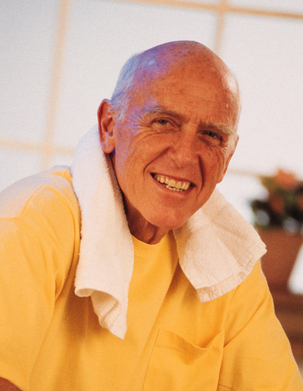
\includegraphics[width=\marginparwidth]{img/personas/elderly.jpg}
	\medskip
	\begin{description}[leftmargin=3cm]
		\item[Name] Howard Evans
		\item[Occupation] Retired
		\item[Age] 65
	\end{description}

	\subsection*{Main Goals}
	\begin{itemize}[leftmargin=1em]
		\item Increase his overall physical activity.
		\item Maintain his independence from his wife.
		\item Limit his time using computers.
		\item Pay for the activity at the venue.
	\end{itemize}
}

\subsubsection*{Description}
\label{ssub:eldery_description}

Howard lives on the outskirts of York with his wife. Howard's wife works most
days of the week as a supermarket shop assistant and their youngest son has now
left home for university in London, leaving Howard with a lot of spare time on
his hands. To help stay connected with his dad, Howard's son has bought him a
smartphone in spite of Howard's inexperience and frustration with technology.
For this reason he also prefers not to put any sensitive information in his
phone, like credit card information.

Though Howard was very active in his working years, he has come to enjoy a more
sedate life since retiring last year from his job as a construction manager.
Recently diagnosed with osteoarthritis, Howard has been advised to exercise
more regularly to help strengthen his muscles and joints. Howard has always
been competitive, and would happily try his hand at any sport he could find.
However, joint pain in his knees often restricts him from some high impact
activities.

No longer able to drive, Howard relies on walking and public transport to get
around during the week when his wife is not at home to drive him.

% subsubsection description (end)

\subsubsection*{Scenarios}
\label{ssub:eldery_scenarios}

\begin{itemize}
	\item Howard's doctor has just told him he needs to start doing more
        activity. Howard has a lot of free time, but he doesn't know what
        sports he wants to play and doesn't know what facilities there are in
		York so he searches on his phone to see what his options are.

	\item Howard has gathered a group of 4 old friends to play sport with him
		this Friday when they are all free. They're happy to play anything
		involving a racquet. If it goes well, he wants to make it a regularly
		weekly activity.

	\item Howard has been having a lot of knee pain over the last few days so
        his doctor has suggested he try swimming. He doesn't think he can
		travel too far from his house and is worried he would need disabled
        access at the pool and doesn't want to feel rushed at the pool by
		younger and faster swimmers.
\end{itemize}

% subsubsection scenarios (end)

\subsubsection*{Pain Points}
\label{ssub:eldery_pain_points}

\begin{itemize}
	\item joint pain in his hands often causes difficulty and discomfort when
		using his mobile phone.
	\item has very little patience with technology.
	\item would often prefer to play close to public transport facilities.
	\item joint pain in his knees often makes walking up stairs very
		uncomfortable.
\end{itemize}

% subsubsection pain_points (end)

%Reference: http://www.theconstructionindex.co.uk/news/view/pay-now-argue-later
\subsection{Working Persona}
\label{sub:working_persona}

\marginpar{%
	\null
	\includegraphics[width=\marginparwidth]{img/personas/working.jpg}
	\medskip
	\begin{description}[leftmargin=3cm]
		\item[Name] Janet
		\item[Occupation] IT Consultant
		\item[Age] 33
	\end{description}

	\subsection*{Main Goals}
	\begin{itemize}[leftmargin=1em]
		\item To play sport on her way home from work and at weekends
		\item To ease the stress of work and recent break-up
		\item Get involved in group sports to meet new people
	\end{itemize}
}

\subsubsection*{Description}
\label{ssub:working_description}

Janet lives in a flat in Sheffield but must commute to Leeds during the week
for work. Her job as an IT consultant  can be stressful and very time consuming
and often requires working late into the evenings. Due to her busy work
schedule, Janet is restricted to playing sport on occasional evenings and at
weekends. She doesn't have any children and currently lives on her own after
recently coming out of a long term relationship. And for that reason, she wants
to get out of the flat as much as possible and take her mind off things by
staying busy and active.

Janet wants to play sport on her drive home from work as she does not have time
to go home first. The fact she has a reasonably long commute gives Janet a
large area in which she can play sport, and therefore a greater selection of
sport centres to choose from. Due to her successful career, Janet has a decent
income so is not restricted by budget and is willing to pay extra for playing
at peak times. Her eagerness to stay active and keep busy means she is very
much up for playing any sports, even if she has never played them before.

Although Janet works in the IT industry, her experience with using
applications on a smart phone is limited.

% subsubsection description (end)

\subsubsection*{Scenarios}
\label{ssub:working_scenarios}

\begin{itemize}
	\item Janet feels like playing a team sport on Friday, she doesn't mind
		what sport but doesn't fancy doing something on her own. She has two
		friends who would like to get involved but would be willing to join
		other groups. The friends live far away and when they are organising
		the event, they would like to be able to share the same screen to make
		finding a suitable booking easier.

	\item It's a Tuesday evening and Janet has a table tennis session booked
		for 7pm. She has just been called in to an urgent meeting at work and
		doesn't think she can make the timeslot she has booked. She would like
		to see if she can push her timeslot back an hour, if not she must
		cancel.

	\item Janet has checked the weather forecast for next Saturday and it is
		looking to be a beautiful day. She has a coffee date at 2pm so can play
		any time before then and would like to play a sport outside.
\end{itemize}

% subsubsection scenarios (end)

\subsubsection*{Pain Points}
\label{ssub:working_pain_points}

\begin{itemize}
	\item Unpredictable work schedule.
	\item Does not want to travel far from her usual commute route to get to a
		center to play sports.
	\item Can't plan for playing sports very far in advance.
\end{itemize}

% subsubsection pain_points (end)

\newpage
% Image reference: http://www.getfurther.co.uk/benefits_skills.php
\subsection{Student Persona}
\label{sub:student_persona}

\marginpar{%
	\null%
	\includegraphics[width=\marginparwidth]{img/personas/student.jpg}
	\medskip
	\begin{description}[leftmargin=3cm]
		\item[Name] Jenny Stevens
		\item[Occupation] Student
		\item[Age] 20
	\end{description}

	\subsection*{Main Goals}
	\begin{itemize}[leftmargin=1em]
		\item To fit tennis around her timetable on a regular basis
		\item To find cheap sports facilities locally
	\end{itemize}
}

\subsubsection*{Description}
\label{ssub:student_description}

Jenny is a 20-year-old university student. She began playing tennis
over the summer and would like to start playing regularly, she is not
interested in any other sports.

Her university is situated in a large city. Jenny lives in a shared
house close to the university's campus. As a student, she has a limited
budget and would prefer to play somewhere close to the university. This
would keep her travel costs down and she would be able to fit in a
round of tennis in between attending lectures. She would also prefer
places that would offer her a student discount or reduced price for
multiple bookings.

Jenny organises her daily activities and social events on her mobile
phone and would find it convenient to book sports facilities and keep
track of her bookings through an app.

% subsubsection description (end)

\subsubsection*{Scenarios}
\label{ssub:student_scenarios}

\begin{itemize}
	\item This semester, Jenny has no lectures on Monday mornings,
		Wednesday afternoons and between 11am and 2pm on Thursdays.
		She would like to book a tennis court for one of these times.

	\item Jenny has a major assessment deadline next week and decides
		to spend her time during the day working. However, she would
		like to book for an evening session for any day during the
		week on a clay court in order to prepare for an upcoming
		tournament.

	\item She is practicing for a tournament with a friend and they have
		agreed to play together every week. In order to help remind her
		friend of this, Jenny would like to send the booking details when she
		has booked the court and have a weekly reminder of the time.
\end{itemize}

% subsubsection scenarios (end)

\subsubsection*{Pain Points}
\label{ssub:student_pain_points}

\begin{itemize}
	\item Jenny is only interested in tennis, and sometimes finds it
		difficult to locate this amongst all the other sports on offer

	\item She has a limited budget; she would prefer facilities that
		provide student discounts or other offers

	\item She would like to use sports facilities within walking
		distance from university, to fit around her timetable and to
		keep travel costs down
\end{itemize}

% subsubsection pain_points (end)

\newpage
\subsection{Child Persona}
\label{sub:child_persona}

\marginpar{%
	\null%
	\includegraphics[width=\marginparwidth]{img/personas/child.jpg}
	\medskip
	\begin{description}[leftmargin=3cm]
		\item[Name] Joe Wyatt
		\item[Occupation] School student
		\item[Age] 14
	\end{description}

	\subsection*{Main Goals}
	\begin{itemize}[leftmargin=1em]
		\item Stay active and have fun playing sports, with his father if
			possible.
		\item Try out new sports
		\item Make friends
	\end{itemize}
}

\subsubsection*{Description}
\label{ssub:child_description}

Joe lives at home in a small town with his father, Pete. He is very active,
playing many sports at school and outside and enjoys trying new sports whenever
the opportunity is available. His father is keen to encourage him to
participate in a wide range of activities so that he can make friends and stay
fit.

Joe is at school every day, but has afternoons after school, and the weekends
available. His father tries to find times when they can spend time together so
sometimes take an afternoon off work to play sport with Joe.

Pete commutes just a short way to work by car, so doesn't mind travelling a bit
to find some good facilities and has also been very active in the past so is
always up for trying out new sports.

Joe is very adept with the latest technology, but occasionally has difficulty
with words and colours since he has very mild dyslexia and red-green
colorblindness.

% subsubsection description (end)

\subsubsection*{Scenarios}
\label{ssub:child_scenarios}

\begin{itemize}
	\item With summer approaching, Joe wants to start a new sport outside and
		his dad wants him to have a professional coach. He's not too concerned
		what it is, but it needs to be close to home, as he'll need to get the
		bus there.

	\item Its the end of term and Joe wants to organise a squash tournament
		with a group of friends and his Dad. They want to book a couple of
		courts nearby for after school during the week, but they're not to
		concerned about the day.

	\item Pete and Joe want to play a game of tennis, but the court they
		sometimes go to is not of great quality. This time, they don't mind
		going further, and want to spend a bit more to get really good courts.
\end{itemize}

% subsubsection scenarios (end)

\subsubsection*{Pain Points}
\label{ssub:child_pain_points}

\begin{itemize}
	\item Sometimes has difficulty reading small text with bad colours.
	\item Pete is keen to get a good deal whenever possible, but not at the
		expense of good facilities at the right time.
\end{itemize}

% subsubsection pain_points (end)


% section user_personas (end)

\part{First Generation Prototypes}
\label{sec:first_prototypes}

The design process is aided by the generation and evaluation of a number of
first and second generation prototypes. These will be assessed against several
specific criteria as well as the user personas defined in Section~%
\ref{sec:user_personas}. Using the results from these evaluations, the
best aspects of the first prototypes will be used to inform the second
generation.

When evaluating the initial designs, each of the potential scenarios are
examined and the prototype tested to see if it provides the required or desired
functionality. In addition to theses real world situations, the designs are
tested against a set of heuristics called Neilsen’s heuristics which

\begin{description}

	\item[Visibility of system status] the activity that is currently being
		performed should be clear to the user, and the status of that activity
		should be clear. For example, if a process is running, waiting, or
		completed.

	\item[Match between system and the real world] using standard conventions
		for ordering items makes them easier to search through and select. Also
		the wording of buttons, labels and information should be familiar to
		the user. However, the computer system should not try to immitate a
		physical object directly, i.e.\ skewomorphism.

	\item[User control and freedom] the user should be in control of the
		system. The system should work for them, but provide the ability to
		undo mistaken actions.

	\item[Consistency and standards] any methods for interacting with the
		system should be uniform accross different platforms so that users do
		not need to relearn to use the system.

	\item[Error prevention] reducing the possibility of errors, and the ability
		for the user to provide data that could cause an error is better than
		recovering from errors. If an error does happen, then giving the user
		information is generally better than leaving them without knowing what
		happened.

	\item[Recognition rather than recall] having navigational elements clearly
		visible and reachable means that the user does not need to remember how
		to use the application, instead the instructions are effectively
		onscreen.

	\item[Flexibility and efficiency of use] catering to advanced users without
		distracting or confusing the novice allows the system to be used by a
		wider range of people.

	\item[Aesthetic and minimalist design] including irrelevant data, or
		information that is only needed infrequently can be distracting.
		Reducing the number of visual stimulii presented to the user can
		increase speed and efficiency.

	\item[Help users recognize, diagnose, and recover from errors] easy to
		read, simple error messages, briefly explaining what happened can help
		the user to not get into the same situation again.

	\item[Help and documentation] providing documentation in a well structured
		way can help the tentative user to use the basic functionality and the
		advanced user find more.

\end{description}

\subsection{Prototype 1}

\subsubsection{Presentation}
\textbf{Tools:} proto.io

\paragraph{Rationale}
This prototype focuses on a content driven display showing users immediately
what is available local to them with interactive tools for adjusting their
search.

\paragraph{Home Map}

\marginFig{img/firstPrototypes/Pro1Home}{The home map screen}{fig:Pro1Home}
On opening the app, the user is immediately shown this map home screen with the
date and time set to the current time and the location centred on the user's
location.
\begin{enumerate}
	\item The tab bar links to pages where the user can decide which sports and
		dates to filter into the search. The location tab will prompt the user
		to enter a new postcode to centre the map on or ask them if they would
		like to reset to their current location.
	\item Icons represent locations to play sport. Where a single sport is
		available to play at a location, a picture for that sport is shown.
		Where more than one sport is available, a plus sign is show to indicate
		that several sports are available at that location. When a user presses
		a sports icon, they are shown the book now screen.
	\item Colour shows, using a traffic light scale, either:
		\begin{enumerate}
			\item availability of courts/facilities. Green indicates there is
				full availability at the location where red indicates there is
				only one booking left at this time.
			\item price of bookings at this location. Green indicates all
				bookings are free at this location and red indicates prices are
				expensive (in comparison to other activities in the area).
		\end{enumerate}

	\item Settings button brings up a small drop down box to ask the user which
		of the two options they would like colour to indicate, availability or
		price.
	\item Map is navigable in the same way as the phone's native map
		application.  The user can zoom in and out with finger gestures and pan
		left, right, up and down. As the user changes their location/zoom
		level, the sports icons update to cover the new area.
	\item The current day being shown, with arrows to navigate through all days
		which are selected in the dates tab. By default, this is all dates, but
		the user can filter the dates via the dates tab.
	\item A time slider which can be moved in hour increments. The icons shown
		on the map will change to accurately show what bookings are available
		for the hour following whatever time this slider is set to by the user.
	\item A weather prediction for the date and time currently selected.
\end{enumerate}

\paragraph{Sports filter}

\marginFig{img/firstPrototypes/Pro1Sports}{Sports filter screen}{fig:Pro1Sports}
A page to filter which sports are shown on the map home page.

\begin{enumerate}
	\item Buttons for quickly selecting or deselecting all sports.
	\item Checkboxes; when ticked, the chosen sports are included in the
		search.
	\item A bar that can be either pressed or dragged up to close the sports
		selection tab and return to the map home page.
	\item The tab bar remains so the user can navigate between sports, date and
		location selection without having to do so via the home screen.
\end{enumerate}

\paragraph{Dates filter}

\marginFig{img/firstPrototypes/Pro1Dates}{Dates filter screen}{fig:Pro1Dates}
A page to filter which dates are included in the search. Dates which are
highlighted are included in the date navigation on the map home page. (no 4 on
the home screen)

\begin{enumerate}
	\item Arrows to move between months of the year.
	\item Days of the month. A user can press a number to highlight it, or
		swipe around the screen to highlight several dates in one swipe, e.g.\
		swiping across a whole row to highlight an entire week.
	\item Days of the week. A user can press one of these days, such as M for
		monday, to highlight every occurrence of that day in the month.
	\item A bar that can be either pressed or dragged up to close the dates
		selection tab and return to the map home page.
	\item The tab bar remains so the user can navigate between sports, date and
		location selection without having to do so via the home screen.
\end{enumerate}

\paragraph{Book now screen}

\marginFig{img/firstPrototypes/Pro1Booking}{Book now screen}{fig:Pro1Booking}
This screen appears when a user selects a sports icon on the home page. The
screen does not cover the whole of the previous page, allowing the user to
still see the date of the booking and the weather prediction for that time. The
user can press the x to close this screen and return to the search.

\begin{enumerate}
	\item The sport available at this location. If several sports are available
		at this location, a drop down arrow is show next to the sport name to
		allow the user to select other sports at that location.
	\item User can get directions through their phone's native map application,
		call the reception of the offices to get more information or navigate
		through pictures of the facilities.
	\item The user can still attempt to change the time or date on the screen.
		If a booking slot is available at the newly selected time then details
		on the book now screen will change to reflect the change in time and
		price (if applicable). If a booking is not available then the text
		between the sport name and `Location Details' will be replaced by a
		message telling the user no booking is available at this time.
	\item The `Book Now' can be pressed to take the user to an external pay
		site or the website of that sports facility to pay for the booking.
\end{enumerate}

\newgeometry{left=3cm}
\subsubsection{Evaluation}

\begin{center}
	\renewcommand{\arraystretch}{2}
	\begin{longtable}{p{0.3\textwidth} c p{0.6\textwidth}}
		\toprule
		\textbf{Criteria} & \textbf{Rating} & \textbf{Comment}\\
		\midrule
		Visibility of system status & $+$ & The time and date of the current
		results are always shown on the home screen.\\

		Match between system and the real world & + & Map applications have
		become ubiquitous so use of the map should be intuitive.\\

		User control and freedom & 0 & There are intuitive ways to return to
		previous screens and navigate between screens. However, an undo or
		return button could be added to return a user to a previous page they
		were on.\\

		Consistency and standards & $-$ & May not be clear that the dates on
		the map screen correspond to those in the dates filter tab.\\

		Error prevention & 0 & Relatively few screens reduces the number of
		places an error can be made. Ensure there is a confirmation message
		before letting the user book facilities.\\

		Recognition rather than recall & 0 & Clear icons are used to indicate
		each sport. No indication on map screen of which dates they can scroll
		through unless they go to the dates tab to see selected dates.\\

		Flexibility and efficiency of use & 0 & Swiping on dates filter tab can
		speed up date selection. No bulk booking, if user knows they want to
		make several bookings, they have to search and process each
		indiviually. \\

		Aesthetic and minimalist design & + & Keeping sports and date filters
		tabs separate from map results and grouping icons when several sports
		are available leaves map search results clear from clutter.\\

		Help users recognize, diagnose, and recover from errors & $-$ & If a
		user changes time or date on the booking screen they will be shown a
		message if a booking is not available at that time. However, there is
		no undo button to return to the original selection.\\

		Help and documentation & $-$ & Currently no descriptions or tutorials
		telling the user how to use they system. Could add a help icon which
		allows users to see what each page does or an initial tutorial on first
		use of the application.\\
		\bottomrule
	\end{longtable}
\end{center}

\begin{center}
	\renewcommand{\arraystretch}{2}
	\begin{longtable}{p{0.12\textwidth} p{0.3\textwidth} c p{0.45\textwidth}}
		\toprule
		\textbf{User} & \textbf{Scenario} & \textbf{Rating} & \textbf{Comment}\\
		\midrule
		\textbf{Elderly} & Searching for new sports in the area & 0 & Howard is
		given an immediate visual representation of what sports are available
		near him when opening the app. However, with his lack of experience
		with technology, use of the map may not be intuitive to him and he may
		prefer options to read results as a list.\\

		& Raquet sport with 4 friends on friday & 0 & Howard could tick only
		racquet sports on the sports filter tab and fridays on the dates tab.
		However, there is no way for him to bulk book if he wants to regularly
		play.\\

		& Swimming nearby with knee pain & $-$ & There is currently no way to
		search for facilities that have disabled access. This could be included
		in the description of the facility on the booking page but Howard would
		still have to look at each search result individually.\\

		\midrule
		\textbf{Working} & Team sport on friday & + & Janet can select the
		relevant sports and dates to show relevant results.  Could have quick
		buttons on the sports tab screen to quick select all team sports to
		speed this up.\\

		& Change/cancel booking at late notice & $-$ & As booking payments are
		held outside the application there is currently no way to cancel
		bookings or even see previous bookings. Could add a screen to add
		favourite booking slots to so users can potentially see previous
		bookings.\\

		& Outdoor sport early saturday & + & Janet can select the relevant
		sports and dates to show relevant results.Could have quick buttons on
		the sports tab screen to quick select all outdoor sports to speed this
		up. The weather prediction on the map screen also helps inform her
		search here.\\

		\midrule
		\textbf{Student} & Tennis court at specific times & + & Jenny can
		select tennis from the sports tab and all preferred dates from the
		dates tab and then quickly browse through her options on the map. \\

		% across different times at the weekend.\\
		& Weekday evening session & + & Jenny can select all days from the date
		tab then set the time to evening on the map and scroll through each day
		seeing which day suits her best.\\

		\midrule
		\textbf{Child} & Outdoor sport close to home or on a bus route & 0 & If
		Joe chooses his preferred outdoor sports from the sports tab, he will
		be shown those close to him straight away. However, there is no
		indication of bus routes on the map. An option could be added to
		overlay local bus routes on the map.\\

		& Booking several squash courts for after school tournament & $-$ &
		There is no way for Joe to book several courts at one time or several
		dates at one time. Could add an option on the booking screen to book
		several courts at once or add a basket function so users can select all
		the bookings they want and then pay for them together.\\

		& Could have some kind of rating system to the location description on
		the bookings page and some way to search for highly rated locations.\\
		\bottomrule
	\end{longtable}
\end{center}
\restoregeometry%

\subsubsection{Conclusion}

%\noindent Description of features to take forward + changes that can
%be made to these features and features to avoid because of their failings
%etc.

\newpage
\subsection{Prototype 2}

\subsubsection{Presentation}
\textbf{Tools:} balsamiq

\paragraph{Rationale}
This prototype is a hierarchical design displaying each screen as a series of
steps which the user must progress through before searching. This prototype
also focuses on a very simple, easy to use interface.

Choose all criteria before searching

\paragraph{Home Screen}
\marginpar{%
	\begin{overpic}[width=0.8\marginparwidth]
		{img/firstPrototypes/Pro2Home_Screen}
		% \put(-7,94){\framebox{1}}
		% \put(62,70){\framebox{2}}
		% \put(3,22){\framebox{3}}
		% \put(46,23){\framebox{3}}
		% \put(62,92){\framebox{4}}
		% \put(5,45){\framebox{5}}
	\end{overpic}
	\captionof{figure}{The home screen}\label{fig:Pro2Home_Screen}
}

The home screen offers a choice of three menus

\begin{enumerate}
	\item Make a booking; takes users to the hierarchy of search screens to
		enter their criteria
	\item Change a booking; takes the user to a screen which allows them to
		change their criteria if alternative results permit it
	\item Cancel booking; takes the user to a screen of their current bookings
		and the user can select which booking they would like to cancel.
		Whether a refund is possible would depend on the sport centre
\end{enumerate}

\paragraph{Search screen 1}
\marginpar{%
	\begin{overpic}[width=\marginparwidth]
		{img/firstPrototypes/Pro2First_Screen}
		% \put(-7,94){\framebox{1}}
		% \put(62,70){\framebox{2}}
		% \put(3,22){\framebox{3}}
		% \put(46,23){\framebox{3}}
		% \put(62,92){\framebox{4}}
		% \put(5,45){\framebox{5}}
	\end{overpic}
	\captionof{figure}{First search screen}\label{fig:Pro2First_Screen}
}

On selecting `Make a booking', the user will be directed to the initial search
screen which will be the first step in their search

\begin{enumerate}
	\item The help button takes the user to a guide on how to complete the
		current page along with FAQ's.
	\item The progress bar shows the user how far along they are in the search
		process.
	\item The user can choose which sport they would like to play from a drop
		down menu. The drop down menu shows recent search results at the top,
		then list all available sports in alphabetical order.
	\item The user must press on the calendar icon which will present them with
		a calendar to select which date they would like to play.
	\item The time is chosen by selecting the hour and minutes from drop down
		bars.
	\item The user can select how long they would like to play for, chosen from
		a drop down bar with half hour intervals.
	\item Takes the user to the next step in the search process.
\end{enumerate}

\paragraph{Search screen 2}
\marginpar{%
	\begin{overpic}[width=0.8\marginparwidth]
		{img/firstPrototypes/Pro2Second_Screen}
		% \put(-7,94){\framebox{1}}
		% \put(62,70){\framebox{2}}
		% \put(3,22){\framebox{3}}
		% \put(46,23){\framebox{3}}
		% \put(62,92){\framebox{4}}
		% \put(5,45){\framebox{5}}
	\end{overpic}
	\captionof{figure}{Second search screen}\label{fig:Pro2Second_Screen}
}

The next screen focuses on location.

\begin{enumerate}
	\item The search box allows the user to specify their location by either
		town, city or postcode. When the user begins to type a location, the
		system will suggest locations based on what they have already typed
	\item The user can use a horizontal slider to specify how far they are
		willing to travel to play the sport
	\item If the user requires disables access they can tick the checkbox and
		the results will only show sports centres which are wheelchair
		accessible
\end{enumerate}

\paragraph{Search Screen 3}
\marginpar{%
	\begin{overpic}[width=0.8\marginparwidth]
		{img/firstPrototypes/Pro2Third_Screen}
		% \put(-7,94){\framebox{1}}
		% \put(62,70){\framebox{2}}
		% \put(3,22){\framebox{3}}
		% \put(46,23){\framebox{3}}
		% \put(62,92){\framebox{4}}
		% \put(5,45){\framebox{5}}
	\end{overpic}
	\captionof{figure}{Third search screen}\label{fig:Pro2Third_Screen}
}
The user is then brought to the final search screen where they may be able to
get discounts

\begin{enumerate}
	\item Numeric stepper to specify how many people the booking is for.
	\item The user may be eligible for discounts if they are a child, student
		or pensioner. They can tick the suitable checkboxes if they fall into
		any of these categories.
	\item If the user has a strict budget, they can choose to only see results
		which do not exceed a  particular price.
	\item Pressing the search button takes the user to a screen displaying the
		results of the search.
\end{enumerate}

\paragraph{Results Screen}
\marginpar{%
	\begin{overpic}[width=\marginparwidth]
		{img/firstPrototypes/Pro2Results_screen}
		% \put(-7,94){\framebox{1}}
		% \put(62,70){\framebox{2}}
		% \put(3,22){\framebox{3}}
		% \put(46,23){\framebox{3}}
		% \put(62,92){\framebox{4}}
		% \put(5,45){\framebox{5}}
	\end{overpic}
	\captionof{figure}{Results screen}\label{fig:Pro2Results_Screen}
}
Screen showing the results of the search

\begin{enumerate}
	\item The user can sort the results by distance, price or time.
	\item If the results are not suitable, the user may wish to change their
		search criteria, the `amend search' button will take them back to the
		first search screen where they can alter their original preferences.
	\item Each result informs the user of the time, date, venue name, distance
		from the venue and the price. The price shows the total price for all
		people. The user can scroll down the page to view all matching results.
	\item Pressing the buttons displaying the price will take the user to a
		more detailed description of the booking and a link to an external pay
		site or the website of that sports facility to pay for the booking.
\end{enumerate}

\newpage
\subsubsection{Evaluation}

\begin{center}
	\begin{adjustwidth*}{}{-3cm}
	\renewcommand{\arraystretch}{2}
	\begin{longtable}{@{\extracolsep{\fill}}p{0.3\linewidth} c p{0.6\linewidth}}
		\toprule
		\textbf{Criteria} & \textbf{Rating} & \textbf{Comment}\\
		\midrule
		Visibility of system status & $+$ & Each screen shows the user their
		progress in the search process \\

		Match between system and the real world & $+$ & Each field is self
		explanatory and is clear what is asked of the user.  \\

		User control and freedom & $-$ & The hierarchical nature of the system
		prevents the user from switching screens easily. If they choose to go
		back they will lose the information they have already typed on the
		screen they left. Freedom is also restricted as the user is required to
		fill all fields. For example they must pick a particular sport at a
		particular time. \\

		Consistency and standards & $-$ & The way users specify their criteria
		varies throughout the search, for example horizontal sliders and
		steppers to achieve numerical values. Although this would not reduce
		the clarity of what is asked of the user. \\

		Error prevention & + & Due to the large buttons and very simple
		interface, there is very little chance of user error. Although the drop
		down menus could get a little fiddly. If the user does accidentally
		book the wrong option, they may have the opportunity to change or
		cancel this booking. \\

		Recognition rather than re-call & $+$ & Information required on the
		current search screen does not depend on information on the previous
		screen. \\

		Flexibility and efficiency use & 0 & Lacks efficiency due to the fact
		that the user must progress through all search screens filling in all
		fields before they can search. \\

		Aesthetic and minimalist design & $+$ & The design is very simple so as
		not to cause any confusion to the user \\

		Help users recognize, diag-nose, and recover from errors & $+$\ & If
		the user tries to move to the next screen having not filled a field or
		filled it incorrectly,  they will be shown a descriptive error message
		in red above that field \\

		Help and documentation & $+$ & The help button displayed on every
		screen takes the user to a guide on how to complete the current page
		along with FAQ's \\
		\bottomrule
	\end{longtable}
\end{adjustwidth*}
\end{center}

\begin{center}
	\begin{adjustwidth*}{}{-3cm}
	\renewcommand{\arraystretch}{2}
	\begin{longtable}{@{\extracolsep{\fill}}p{0.3\linewidth} c p{0.6\linewidth}}
		\toprule
		\textbf{Scenario} & \textbf{Rating} & \textbf{Comment}\\
		\midrule
		\midrule
		\multicolumn{3}{l}{\textbf{Elderly}}\\
		\cmidrule(r){1-3}
		Searching for new sports in the area and notifying his wife of the
		booking. & $-$ & Howard may find using the drop down menus difficult
		with his osteoarthritis. There is no feature to notify people of the
		booking \\

		Racquet sport with 4 friends on Friday & 0 & Can select four people
		to play using drop down menu. Would have to specify which racquet sport
		he wishes to play. No bulk book feature. \\

		Swimming nearby with knee pain & $+$ & If Howard does not wish to
		travel far he can either filter the results by distance or specify a
		maximum distance he is willing to travel (search screen2). If Howards
		knee pain is particularly bad he may wish to swim somewhere which
		doesn't require climbing any stairs. He can do this by ticking the
		wheelchair accessible checkbox. \\

		\midrule
		\multicolumn{3}{l}{\textbf{Working}}\\
		\cmidrule(r){1-3}
		Team sport on Friday including screen sharing with friends & $-$ & The
		app would not support this scenario as there is no option to search for
		just team sports. There is also no current feature to support screen
		sharing but this could be incorporated into the final design. \\

		Change/cancel booking at late notice & 0 & Janet has this option on
		the home screen. Although the app cannot guarantee the venue allows
		cancellations \\

		Outdoor sport early on Saturday & 0 & Useful as Janet can specify a
		time. But again, there is no flexibility in choosing a sport. \\

		\midrule
		\multicolumn{3}{l}{\textbf{Student}}\\
		\cmidrule(r){1-3}
		Tennis court at specific time & $+$ & This scenario is tailored this
		prototypes design. Jenny can specify that she would like to play tennis
		at a particular time on a particular day and how long she would like to
		play for \\

		Weekday evening session must be on clay & 0 & This could be something
		to incorporate on the screen showing the booking in more detail, along
		with other information such as court number \\

		Weekly practice with friend with reminders & $-$ & There is no
		notification feature with this prototype. The regular weekly booking
		feature could also be something that is incorporated in the screen
		showing more detail about the booking. \\

		\midrule
		\multicolumn{3}{l}{\textbf{Student}}\\
		\cmidrule(r){1-3}
		Outdoor sport close to home or on a bus route with coach & $-$ & No
		feature showing any transport routes. Joe would also have to specify
		which outdoor sport he is interested in playing \\

		Booking several squash courts for after school tournament & $-$ &
		With the current design, Joe would have to use the number of players
		field (4 people = 1 court) to portray how many courts he needs. He can
		specify how long they need the courts based on how long they think
		tournament will last. However he would need to choose a particular day.
		\\

		Looking for high quality tennis court & $-$ & There is currently no
		way of finding the quality of the sport facilities. Pete can however,
		use the sliders to increase the maximum distance and price they are
		willing to pay. \\
		\bottomrule
	\end{longtable}
	\end{adjustwidth*}
\end{center}

% \newpage
\subsection{Prototype 3}
\label{sub:prototype_3}

\subsubsection{Presentation}
\textbf{Tools:} proto.io

\paragraph{Rationale}

This prototype is based on the `flat' design of other booking apps. The search
criteria is spread across a number of pages and results are displayed as a
list.

\paragraph{Home Screen}
\marginpar{%
	\begin{overpic}[width=\marginparwidth]
		{img/firstPrototypes/Pro3Main}
	\end{overpic}
	\captionof{figure}{Home screen is also the search page}\label{fig:Pro3Home}
}

The home screen is also a search page. Users are able to search by sport,
location, distance, date and time or a combination of these options; all of
these have the default value of `Any' if the user decides not to enter a
specific value or range.

By selecting a search option, such as `sport', the user will be directed to
another page where they can specify a sport or combination of sports using a
checklist interface similar to the previous prototypes. The `date' section
would allow the user to select a specific date, a variety of dates or between
two dates using a calendar interface. The user can select a time-frame. E.g.
after 5pm, before 12pm or between 4pm and 8pm using the `time page'. Distance
can also be selected by range (e.g.\ up to 5 miles). Location can be selected
from a drop-down list of cities, the user can also type their location or use
GPS for their current location.

Once the user has selected their options they can use the `Search' button to
see their results.

\paragraph{Details}
\marginpar{%
	\begin{overpic}[width=\marginparwidth]
		{img/firstPrototypes/Pro3Details}
	\end{overpic}
	\captionof{figure}{Details screen}\label{fig:Pro3Details}
}

The `Details' button in the navigation bar can store information about the user
such as their age, which can help them to find offers that are relevant to them
or discounts can be applied to the price during the search.

Basic information about the user can be stored locally to apply discounts and
include relevant offers.

\paragraph{Results}
% \marginpar{%
% 	\begin{overpic}[width=\marginparwidth]
% 		{img/firstPrototypes/Pro3Results_1}
% 	\end{overpic}
% 	\captionof{figure}{Results displayed as a list}\label{fig:Pro3Results_1}
% }

The results page allows the user to see their search criteria as well as a list
of available facilities. These can be sorted by price or distance.

The user can go back to change the search criteria using the `Back' button on
the navigation bar or select one of the results in the list for more
information.
% \marginpar{%
% 	\begin{overpic}[width=\marginparwidth]
% 		{img/firstPrototypes/Pro3Results_2}
% 	\end{overpic}
% 	\captionof{figure}{Further information is available}\label{fig:Pro3Results_2}
% }

Once the user chooses an available result, they can see further information on
the facilities selected such as pricing, address, location and contact
information. The user can choose to `share' this information with others or
`book' the facilities using the buttons at the bottom of the screen.

The user can find out more about their current bookings by selecting them from
the main `bookings' page. For previous bookings, the `cancel' button could
change to `book again'.

\begin{figure}[htbp]
	\centering
	\begin{subfigure}[b]{0.45\textwidth}
		\includegraphics[width=\textwidth]{img/firstPrototypes/Pro3Results_1}
		\caption{Results displayed as a list}\label{fig:Pro3Results_1}
	\end{subfigure}%
	\qquad
	\begin{subfigure}[b]{0.45\textwidth}
		\includegraphics[width=\textwidth]{img/firstPrototypes/Pro3Results_2}
		\caption{Further information}\label{fig:Pro3Results_2}
	\end{subfigure}
	\caption{}\label{fig:Pro3Results}
\end{figure}

\paragraph{Tab bar}

There are two tabs on the bar at the bottom of the screen;
\begin{itemize}
	\item `Offers' tab, shows available offers. A user could choose to use
		this to search for facilities by available offers.
	\item `Bookings' tab, users can keep track of their current and previous
		bookings.
\end{itemize}

\marginpar{%
	\begin{overpic}[width=\marginparwidth]
		{img/firstPrototypes/Pro3Bookings_1}
	\end{overpic}
	\captionof{figure}{The bookings tab}\label{fig:Pro3Bookings_1}
}
\marginpar{%
	\begin{overpic}[width=\marginparwidth]
		{img/firstPrototypes/Pro3Bookings_2}
	\end{overpic}
	\captionof{figure}{Further information is available}\label{fig:Pro3Bookings_2}
}

\fullwidth%
\subsubsection{Evaluation}

\renewcommand{\arraystretch}{2}
% \begin{longtable}{@{\extracolsep{\fill}}p{0.3\linewidth} c p{0.6\linewidth}}
\begin{longtabu}{p{0.3\linewidth} c X}
	\toprule
	\textbf{Criteria} & \textbf{Rating} & \textbf{Comment}\\
	\midrule
	Visibility of system status & $+$ & There are only two states in this
	application --- the search screen and the results page.\\

	Match between system and the real world & $+$ & Most other booking
	applications have a similar layout of a search page followed by a list
	of results (E.g.\ trainline, redspottedhanky). It should be easy for a
	user who is familiar with this format to use this design.\\

	User control and freedom & $+$ & `Back' button in the navigation bar
	allows the user to change elements of the search criteria.\\

	Consistency and standards & $+$ & Information is displayed in a similar
	way throughout the application, e.g.\  Bookings and Results both use
	lists and selecting a particular item in the list leads to a page with
	more specific information.\\

	Error prevention & $-$ & There is no way for a user to tell if they
	have made a mistake or where the errors are. A pop-up notification
	could supply this information when the user presses the `search'
	button.\\

	Recognition rather than recall & $+$ & Search criteria is displayed on
	the main page and in the results section.\\

	Flexibility and efficiency of use & $0$ & Novice users may not find this
	format easy-to-use without instructions.  Experienced users could also
	search for offers, or their current/previous bookings using the tab bar
	in addition to using the home screen. \\

	Aesthetic and minimalist design & $0$ & Keeping the search options on
	different pages prevents the home screen from becoming cluttered.
	However, presenting the results as a list may not be helpful for users
	who do not select a specific sport, date, time or location.\\

	Help users recognize, diagnose, and recover from errors & $-$ & There
	is no way for a user to tell if they have made an error. The only
	option available is to go `back' and change the search criteria.\\

	Help and documentation & $-$ & Currently there are no instructions
	available on how to use the application.\\
	\bottomrule
\end{longtabu}

\renewcommand{\arraystretch}{2}
\begin{longtabu}{p{0.3\linewidth} c X}
	\toprule
	\textbf{Scenario} & \textbf{Rating} & \textbf{Comment}\\
	\midrule
	\multicolumn{3}{l}{\textbf{Elderly}}\\
	\midrule
	Searching for new sports in the area and notifying
	his wife of the booking. & $+$ & Howard can search using the location and
	distance criteria for searching for sports facilities locally. He can
	also send the details of his bookings to his wife by using the `share'
	button.\\

	Racquet sport with 4 friends on Friday & $0$ & Howard can select the
	individual sports from a list, there is no option at the moment for
	racquet sports. He can also choose a Friday, but wouldn't be able to
	bulk book for a regular session in-app.\\

	Swimming nearby with knee pain & $-$ & It isn't possible to search
	for facilities that have disabled access, this could be something to
	include in the `details' section and in the information pages of
	individual sports centres.\\

	\multicolumn{3}{l}{\textbf{Working}}\\
	\midrule
	Team sport on Friday including screen sharing with friends& $-$ & Janet
	can select individual sports like netball, football, etc.\  as there is
	no option for `team sports' and dates. She wouldn't be able to share
	all the results with her friends but could share individual bookings
	she selects.\\

	Change/cancel booking at late notice & $0$ & Using the `Bookings'
	tab, Janet could find her booking and cancel it using the `cancel'
	button, or use the information to contact the sports facility to change
	her booking.\\

	Outdoor sport early on Saturday & $+$ & Currently no quick filters
	for `outdoor' sports, Janet would have to go through the list of all
	possible sports and select those that she knows are outdoors.  Or it
	could be easier for Janet to select Saturday and mornings using the
	date and time sections and see what sports are available.\\

	\multicolumn{3}{l}{\textbf{Student}}\\
	\midrule
	Tennis court at specific times & $0$ & Jenny can select tennis only but
	may have to search a few times to find suitable slots for the different
	times she is free.\\

	Weekday evening session must be on clay & $0$ & Jenny can select the
	whole week and hours in the evenings in the `date' and `time' sections.
	She would have to check individual sports facilities to see the types
	of courts available.\\

	Weekly practice with friend with reminders & $0$ & There isn't a way
	for Jenny to book weekly sessions but could book one session a week and
	share the information with a friend using the `share' button.\\

	\multicolumn{3}{l}{\textbf{Child}}\\
	\midrule
	Outdoor sport close to home or on a bus route with coach & $0$ & It
	currently isn't possible to select `outdoor' sports but he could choose
	a variety of sports in the sports section and can sort by distance. It
	wouldn't be possible to know if the facilities are close to a bus route
	but could check with the facilities by contacting them.\\

	Booking several squash courts for after school tournament & $0$ & It
	isn't possible for Joe to book several courts at one time.

	Could have some kind of rating system to the location description on
	the bookings page and some way to search for highly rated locations.\\

	Looking for high quality tennis court & $0$ & It could be possible to
	include other users ratings of each facility and sort results by these
	ratings.\\
	\bottomrule
\end{longtabu}
\restoregeometry%

% \begin{adjustwidth*}{-4cm}{}
\fullwidth%
\subsection{Conclusion}

Following the evaluation of the first prototypes, there are a number
of features we plan to include in our second prototype.

\begin{center}
	\renewcommand{\arraystretch}{2}
	\begin{longtabu}{c p{0.25\linewidth} X}
		\toprule
		\textbf{Prototype} & \textbf{Feature} & \textbf{Comment}\\
		\midrule
		1 & Map & Intuitive to use due to ubiquitous use in most other
		applications.\\
		1 & Sports icons & Removes clutter from the page; important for a small
		screen. \\
		1 & Date selection \& swiping to select & Allows quick and easy input
		of date selection. \\
		1 & Weather indication & Provides relevant further information for user
		scenarios where an outdoor sport was preferred. \\
		1 & Location details & Provides space to inform user on wheelchair
		access, parking information and weather predictions. \\
		\midrule
		2 & Home screen & Clear options help the user quickly identify what
		part of the application they intend to use. \\
		2 & Booking cancellation & Satisfies user scenarios in cancelling
		booking.  Will add a message to inform the user of particular venue
		rules on cancellation. \\
		2 & Wheelchair accessible search & Satisfies user scenarios where
		disabled access to location was required. \\
		2 & Error messages & Helps users understand how to use the applications
		and gives guidance where they've made errors. \\
		2 & Help button & Provides instructions for users \\
		\midrule
		3 & User details & Allows the user to personalise the application to
		their preferences, speeding up their searches. \\
		3 & Current/previous bookings & Aids the user in both cancelling and
		sharing bookings, both common user scenarios. \\
		3 & Share button & Satisfies user scenarios that requires sharing
		information about a booking with friends/relatives. \\
		3 & Search options non-exhaustive & Matches real world situations and
		user scenarios where the user does not have specific criteria for each
		individual search option. \\
		3 & Back buttons & To an extent, allowed the user to undo some errors
		in navigating through the application. \\
		\bottomrule
	\end{longtabu}
\end{center}
% \end{adjustwidth*}

The evaluations, particularly those against the user scenarios, highlighted a
number of features which are missing from all of the initial prototypes:

\begin{itemize}
	\item The ability to make several bookings at once.
	\item Confirmation messages when performing certain actions, such as making
		a booking.
	\item Grouping sports, such as team or outdoor sports, when searching for a
		sport.
	\item Clarification on booking cancellations as some venues may not allow
		cancellations at all or at least not without a certain amount of
		notice.
	\item Including public transport options in the location search
	\item An indication of location quality, such as through user reviews.
\end{itemize}

\subsection{Evaluation of Tools}

\subsubsection{Proto.io}

Proto.io\cite{protoio} is a useful tool as it's specifically for creating
mobile prototypes.  It has a library of different devices and each has default
UI components, such as buttons and lists built-in. Once a number of screens
have been designed, they can be linked together. For example, a button could
link to the next screen, which helps to visualise how the app could work.

Overall, it has a very easy to use `drag-and-drop' interface, and the gridlines
are helpful in positioning different components.

\subsubsection{Balsamiq}

Based on the simplicity of the prototypes, Balsamiq\cite{balsamiq} was a useful
mock-up tool to use as it allowed the prototype to be completed with a hand
drawn effect.  The selection of pre-drawn widgets were enough to design
everything required of the prototype with the exception of a home page icon.

A major drawback of the tool was the inability to custom design a widget that
was not already available.  This meant there was no way of personalizing our
design.

\subsubsection{Possible Alternatives}

There are a large number of other tools which we could use to develop the
second prototype. These range from applications not specifically designed for
prototyping. There are drawing packages such as Adobe Photoshop, presentation
software such as Microsoft PowerPoint and also software allowing sophisticated
animation and interactivity such as Adobe Flash. These could be used together
or individually to create a prototype.

The drawing package would allow a very high quality appearance for each screen.
However, this would come at a cost of time and effort, particularly for someone
without experience in the particular drawing package being used. Presentation
software would facilitate most basic interaction options between screens but
would likely need to be used in conjunction with a drawing package to a allow
higher quality appearance. More sophisticated animation software would allow
greater interactivity options, but at a significant cost as these tools often
require a lot of prior experience to use effectively and quickly.

\subsubsection{Conclusion}

We will use proto.io as our tool for developing the second prototype. Of all
the options we considered, this tool will allow the highest level of
functionality to be included in the prototype in the least amount of time and
with the least amount of effort. Furthermore, many of the other possible tools
have a learning curve that can increase the time taken to develop the
prototype. The experience gathered from using proto.io in our initial
prototyping will help us avoid this problem. One possible drawback is that this
tool is only free for a limited time through a trial membership.

\restoregeometry%


% section first_prototypes (end)

\clearpage

\fullwidth%
\begin{landscape}
\thispagestyle{plain}
\begin{figure}[p]
	\centering
	\includegraphics[height=\textwidth]{img/secondPrototype/outline.png}
	\caption{Outline diagram showing navigation paths between screens.
		Navigation starts, when the user opens the application, at the home
		screen, shown in the top left.
	}\label{fig:pro2outline}
\end{figure}
\end{landscape}
\restoregeometry%

\part{Second Generation Prototype}
\label{sec:second_generation_prototype}

We have developed a second prototype based on what we have learnt from the
evaluation of our first prototypes. This prototype has more functionality than
any of the first prototypes to allow us to better evaluate the design against
heuristics and scenarios and through usability testing. The basic navigation
between screens is shown in Figure~\ref{fig:pro2outline}, while each screen is
explained in more detail below in Section~\ref{sec:secondprotopresentation}.

\section{Presentation}

Figure~\ref{fig:pro2outline} shows a visual representation of the paths that
are availible for navigating through the application. Each of the screens shown
is explored further below.

\paragraph{Home} (Figure~\ref{fig:HiHome})

\marginpar{%
	\begin{overpic}[width=\marginparwidth]
		{img/secondPrototype/home}
	\end{overpic}
	\captionof{figure}{The Home screen}\label{fig:HiHome}
}

The user is at first presented with three main options to choose from.
\begin{enumerate}
	\item Make a new booking; this button takes the user to a page to input
		their search criteria. (Figure~\ref{fig:HiSearch})
	\item View their bookings; this button allows the user to see past and
		present bookings. (Figure~\ref{fig:HiBookings})
	\item Input their details; this page allows the user to specify a number
		of details about themselves:

		\begin{enumerate}
			\item Their concession status so they potential offers and
				discounts can be highlighted in the search results.
			\item Default search preferences if they regularly search for the
				same sport, location or time when looking to make a booking.
		\end{enumerate}
	\item The home button is repeated on every page and provides the user with
		a quick way to return to this home screen.
\end{enumerate}

\paragraph{My Bookings} (Figure~\ref{fig:HiBookings})

\marginpar{%
	\begin{overpic}[width=\marginparwidth]
		{img/secondPrototype/bookings}
	\end{overpic}
	\captionof{figure}{Current and past bookings screen}\label{fig:HiBookings}
}

This page shows scrollable lists of current and past bookings the user has
made. This allows the user to find details about past bookings if they want to
repeat a search or contact the location. The user may also be able to cancel a
current booking if the particular location they have booked allows them to.

\paragraph{Individual Current Booking Page} (Figure~\ref{fig:HiIndBooking})

\marginpar{%
	\begin{overpic}[width=\marginparwidth]
		{img/secondPrototype/indiv_booking}
	\end{overpic}
	\captionof{figure}{Current booking details screen}\label{fig:HiIndBooking}
}

This page displays information for a current booking.
\begin{enumerate}
	\item A share button; this will display the phone's default share options.
		Typically this will allow the user to share information about the
		booking through other applications on the phone such as email or other
		messaging services.
	\item If the location of this booking allows customers to change booking
		times, this will bring up a search results page, similar to
		figure~\ref{fig:HiList}, showing available booking slots at similar
		times at this location.
	\item The details tab has buttons to call the location, visit their
		website, get directions to the location and also highlights if the
		location has parking facilities. In addition to this, the weather
		prediction for this location at the time of the booking is displayed.
	\item An button to cancel the booking; a prompt will be displayed asking
		the user to confirm that they definitely wish to cancel the booking.
		If the location does not allow booking cancellations, this button will
		be greyed out and attempts to press the button will result in a message
		explaining the reason a cancellation cannot be made.
\end{enumerate}

\paragraph{Search} (Figure~\ref{fig:HiSearch})

\marginpar{%
	\begin{overpic}[width=\marginparwidth]
		{img/secondPrototype/search}
	\end{overpic}
	\captionof{figure}{The main search screen}\label{fig:HiSearch}
}

This is the main search screen which displays the current criteria in the
search and allows the user to change this criteria viewing the results that
match this criteria. The user can choose to search after defining any number of
the four criteria.
\begin{enumerate}
	\item Help button; displays hovering annotations describing what each part
		of the page is for.
	\item Reset search button; this resets the search criteria to the default
		settings chosen on the My Details page. If the user has not entered
		these details before then the sport selection will be default to all,
		location to 5km within the user's current location, date to today and
		time to all.
	\item Past booking button; this brings up a drop down list of previous
		bookings. If one of these bookings is chosen, all the search criteria
		will change to match that booking apart from the date which will remain
		unchanged.
	\item Sport selection button with icons that show what is currently
		selected.  Pressing this leads to figure~\ref{fig:HiSport}.
	\item Location button leading to figure~\ref{fig:HiLocation}.
	\item Date button leading to figure~\ref{fig:HiDate}.
	\item Time button leading to figure~\ref{fig:HiTime}.
	\item Search button leading to figure~\ref{fig:HiList} to display results
		matching the current search criteria.
	\item A basket icon which leads to the basket page which displays all
		booking slots a user currently has added to their basket but have yet
		to confirm and pay for.
\end{enumerate}

\paragraph{Sport Selection} (Figure~\ref{fig:HiSport})

\marginpar{%
	\begin{overpic}[width=\marginparwidth]
		{img/secondPrototype/sport}
	\end{overpic}
	\captionof{figure}{The sport selection screen}\label{fig:HiSport}
}

The user can choose to search for as many sports at once as they wish.
\begin{enumerate}
	\item Drop down to choose to display different groups of sport such as
		outdoor sports, indoor sports, teams sports and favourites which are
		defined on the My Details page.
	\item Select all button; this will check all sports currently displayed on
		the page. If all sports are selected, this button changes to clear all
		instead.
	\item Each sport toggles between selected and unselected when pressed.
	\item Done button; this returns the user to the search page. This the same
		for all specific search criteria pages. (Figure~\ref{fig:HiSearch})
	\item Help button; displays hovering annotations describing what each part
		of the page is for.
\end{enumerate}

\paragraph{Location Selection} (Figure~\ref{fig:HiLocation})

\marginpar{%
	\begin{overpic}[width=\marginparwidth]
		{img/secondPrototype/location}
	\end{overpic}
	\captionof{figure}{The location selection screen}\label{fig:HiLocation}
}

The user can choose to to search within a distance from their current
location or specify a particular location via its postcode or area
name.
\begin{enumerate}
	\item Find location; a button which sets the location using the user's
		current location.
	\item Location input text field; when the chooses the first button, this
		is automatically changed to the postcode of their current location.
		The user can also type in this field. As they are typing, suggestions
		will appear in a drop down box to help speed up their search.
	\item A slider bar to determine how far from the chosen location the user
		would like to search.
	\item Public transport; if the checkbox is ticked, the user can choose
		to search for locations which are within a specified journey time
		on public transport such as local buses and trains.
	\item Checkboxes for including in the search only those locations which
		have disabled access and parking facilities.
	\item Help button; displays hovering annotations describing what each part
		of the page is for.
\end{enumerate}

\paragraph{Date Selection} (Figure~\ref{fig:HiDate})

% \marginpar{%
% 	\begin{overpic}[width=\marginparwidth]
% 		{img/secondPrototype/date}
% 	\end{overpic}
% 	\captionof{figure}{The date selection screen}\label{fig:HiDate}
% }

All dates which are higlighted on this page will be included in the
search.
\begin{enumerate}
	\item Select all; highlights all dates in the shown month. This button
		changes to clear all when all dates are already selected.
	\item Day headings; when a day is pressed, all the dates on the page for
		that day are highlighted.
	\item The user can either touch a date to highlight it or swipe across multiple
		dates to highlight many dates in one go.
	\item Help button; displays hovering annotations describing what each part
		of the page is for including instructions on using swiping gestures
		to select multiple dates.
\end{enumerate}

\begin{figure}[htbp]
	\centering
	\begin{subfigure}[b]{0.45\textwidth}
		\includegraphics[width=\textwidth]{img/secondPrototype/date}
		\caption{The date selection screen}\label{fig:HiDate}
	\end{subfigure}%
	\qquad
	\begin{subfigure}[b]{0.45\textwidth}
		\includegraphics[width=\textwidth]{img/secondPrototype/time}
		\caption{The time selection screen}\label{fig:HiTime}
	\end{subfigure}
	\caption{}\label{fig:time-dateSelection}
\end{figure}

\paragraph{Time Selection} (Figure~\ref{fig:HiTime})

% \marginpar{%
% 	\begin{overpic}[width=\marginparwidth]
% 		{img/secondPrototype/time}
% 	\end{overpic}
% 	\captionof{figure}{The time selection screen}\label{fig:HiTime}
% }

All hours which are highlighted on this page will be included in the
search.
\begin{enumerate}
	\item AM and PM buttons; when the am is pressed all morning hours are toggled
		on or off, likewise for pm.
	\item The user can either touch an hour to highlight it or swipe across
		multiple times times highlight many times at once.
	\item Help button; displays hovering annotations describing what each part
		of the page is for including instructions on using swiping gestures
		to select multiple times.
\end{enumerate}

\paragraph{List Results} (Figure~\ref{fig:HiList})

%\marginpar{%
%	\begin{overpic}[width=\marginparwidth]
%		{img/secondPrototype/list}
%	\end{overpic}
%	\captionof{figure}{The list results screen}\label{fig:HiList}
%}

This is the default view for search results. Results can be sorted
by distance, time or price and grouped by sport or location. The user
can change the default sort and grouping options on their my details
page.
\begin{enumerate}
	\item Button to return to the search page and amend the search criteria.
	\item Toggle buttons to change how the results are sorted.
	\item Toggle buttons to change how the results are grouped. By default,
		the results are not grouped. An example is shown in figure~\ref{fig:HiListGroup}
		of results grouped by sport. When grouped, a user can expand a chosen
		sport to see all results for that particular sport. These items will
		be also be sorted by the chosen sort option.
	\item Scrollable list of results. The user is shown an icon for the sport,
		the name of the location, the time and date of the booking, the price
		and the distance of the location from their chosen search location.
		Selecting a particular booking slot takes the user to the page in
		figure~\ref{fig:HiIndResult}.
	\item Toggle bar for switching between list and map search view. (Figure~\ref{fig:HiMap})
\end{enumerate}

\begin{figure}[htbp]
	\centering
	\begin{subfigure}[b]{0.45\textwidth}
		\includegraphics[width=\textwidth]{img/secondPrototype/list}
		\caption{The list results screen}\label{fig:HiList}
	\end{subfigure}
	\qquad
	\begin{subfigure}[b]{0.45\textwidth}
		\includegraphics[width=\textwidth]{img/secondPrototype/list_group}
		\caption{The grouped list results screen}\label{fig:HiListGroup}
	\end{subfigure}%
	\caption{}\label{fig:listsResults}
\end{figure}

% \marginpar{%
% 	\begin{overpic}[width=\marginparwidth]
% 		{img/secondPrototype/list_group}
% 	\end{overpic}
% 	\captionof{figure}{The grouped list results screen}\label{fig:HiListGroup}
% }

\paragraph{Map Results}

(Figure~\ref{fig:HiMap})

\marginpar{%
	\begin{overpic}[width=\marginparwidth]
		{img/secondPrototype/map}
	\end{overpic}
	\captionof{figure}{The map results screen}\label{fig:HiMap}
}

Results can also be viewed on a map which is navigable in the same
way as the phone's native map application.
\begin{enumerate}
	\item Icons on the map represent a specific venue. If only one sport is
		available at that venue then the picture icon will represent that
		sport. If more than one sport is available, then there will be a plus
		sign to show that multiple sports are available. When pressed, a
		scrollable list is displayed on the screen similar to that in
		figure~\ref{fig:HiListGroup}.
	\item Toggle bar to navigate back to the list view in
		figure~\ref{fig:HiList}.
\end{enumerate}

\paragraph{Individual Result}

(Figure~\ref{fig:HiIndResult})

\marginpar{%
	\begin{overpic}[width=\marginparwidth]
		{img/secondPrototype/indiv_result}
	\end{overpic}
	\captionof{figure}{Screen for a booking slot}\label{fig:HiIndResult}
}
\begin{enumerate}
	\item Button to add the displayed booking to the user's basket so they can
		continue searching before paying.
	\item Scrollable list of bookings for the same sport and location at the
		same time in future weeks so the user can purchase several weeks at
		once if they know they want to play weekly. The basket icon adds the
		booking to the basket.
	\item Details about the location and a weather prediction for the time of
		the chosen booking.
	\item Book now button; takes the user an external pay application to pay
		for booking before returning them to this page. The book now button
		will then change to a link to the page for this current booking as
		in figure~\ref{fig:HiIndBooking} so they can make amendments to their
		booking at share details to their friends.
\end{enumerate}


\fullwidth%
\section{Review}
\subsection{Evaluation Plan}
\label{sub:evaluation_plan}

Having incorporated aspects of the first generation prototypes based on our
evaluation of them, we will now evaluate our final design using the same
methods as well as using a cognitive walkthrough and a usability questionnaire.

We will begin the evaluation of our second generation prototype by testing it
against Neilsen's heuristics. The main goal of heuristic evaluations is to
identify any problems associated with the design of user interface by means of
a systematic inspection. We would hope to see a reduction in usability problems
compared to the first generation prototypes.

Next will be an examination of the potential scenarios proposed by each
persona. With a more detailed and robust design, we can examine each scenario
in more depth and again hope to see an improvement in the way this prototype
deals with them. We will then apply an inspection method called a cognitive
walkthrough. This is a more formal approach to imagining people's thoughts and
actions when they use an interface for the first time. This allows us to put
ourselves in the shoes of a user while they aim to carry out a particular task
with a certain goal in mind. We will select one task for each persona that the
design is intended to support and then step through each action in that task.
This method should help us find any obstacles a user may face when using the
application having had no experience with it. We must motivate the actions
based on the user's general knowledge and on feedback provided by the
interface.

There are four questions to consider in a cognitive walkthrough\cite{cogwalk}:
\begin{enumerate}
	\item \textbf{Will the customer realistically be trying to do this action?}

	Does the interface make unrealistic assumptions about the level of
	knowledge or experience that users have?

	\item \textbf{Is the control for the action visible?}

	Highlights issues with context-sensitive menus or controls buried too deep
	within a navigation system and identifies non-standard and unintuitive
	icons/buttons.

	\item \textbf{Is there a strong link between the control and the action?}

	Identifies problems with ambiguous or jargon terms.

	\item \textbf{If the correct  action is performed, will the user see that
		progress is being made?}

	Helps to find problems when feedback is unclear, ambiguous or missing
	entirely.

\end{enumerate}
\bigskip

We must decide if each of these questions is a pass or a fail for every action
within the tasks.

Finally we will construct a questionnaire to test usability.  Usability testing
is a technique which will allow us to evaluate our design by testing it on
members of the public. By doing this it allows us to gain a subject assessment.
This is important as having designed the application ourselves, we as designers
know exactly how it works and can make the error of assuming to understand the
user.

We will take an informal approach with our questionnaire by sitting the user
down with the system and letting them use it as they like. Their feedback will
be recorded on the questionnaire and we will use the system usability scale
test to analyse our results and draw any conclusions.

If time restriction was not an issue, there are other inspection methods we
could have applied.  For example, using the consistency inspection method we
could have asked designers who represent multiple other projects to inspect our
interface to see whether it does things in the same way as their own designs.
However, finding designers who represent multiple projects in our time frame is
not plausible.

The feature inspection lists sequences of features used to accomplish typical
tasks, checks for long sequences, unnatural and complicated steps, and steps
that require extensive knowledge and experience in order to assess a proposed
feature set. This method of evaluation would not be beneficial to us as it is
very similar to the cognitive walkthrough and our application does not require
extensive knowledge or experience.

\renewcommand{\arraystretch}{2}
\begin{longtabu}{p{0.3\linewidth} c X}
	\toprule
	\textbf{Criteria} & \textbf{Rating} & \textbf{Comment}\\
	\midrule
	Visibility of system status & $+$ & Clear headings show where in the
	booking process the user is. A simple structure to the pages means that
	returning to the home screen is easy and allows the user to view prior
	bookings.\\

	Match between system and the real world & 0 & Simple, clear, short
	instructions and pieces of information are used to minimise the reading
	onscreen, whilst making the purpose of each selection object clear. The
	sports selection drop down menu is not immediately self explanatory.\\

	User control and freedom & 0 & All stages of the booking allow the user to
	move backwards to a previous state. Since the final booking is handled by
	the independant sports centers, it is up to them to implement some
	verification with the user that the booking details are correct.\\

	Consistency and standards & $+$ & Well recognised icons are used throughout
	which correspond to the same functionality in other applications. \\

	Error prevention & 0 & The settings for the search criteria can all be
	changed before finally selecting `search'. It is not obvious that the time
	of a booking can be changed easily from the bookings screen, and the other
	details of the booking cannot be changed. To do this, the user has to enter
	a new set of search criteria.\\

	Recognition rather than recall & 0 & All icons are chosen to represent the
	function to which they apply to reduce recall. \\

	Flexibility and efficiency of use & $-$ & The user can make repeated
	bookings of for similar searches, but bulk bookings where more than the
	date changes are not possible. \\

	Aesthetic and minimalist design & $+$ & The design is clean and simple with
	bold colours to differentiate sections, headers and icons. There are a lot
	of different icons on the results pages which could make them look
	confusing when the user is not familiar with the structure and layout of
	the page.\\

	Help users recognize, diagnose, and recover from errors & $-$ & There is no
	undo button or selection to revert back to a previous state, the user must
	instead select a new set of search criteria.\\

	Help and documentation & 0 & There is a help button to display information
	about the features available on the current screen.\\
	\bottomrule
\end{longtabu}

\newpage
\renewcommand{\arraystretch}{2}
\begin{longtabu}{p{0.3\linewidth} c X}
	\toprule
	\textbf{Scenario} & \textbf{Rating} & \textbf{Comment}\\
	\midrule
	\multicolumn{3}{l}{\textbf{Elderly}}\\
	\midrule
	Searching for new sports in the area and notifying his wife of the booking.
	& $+$ & If Howard wishes to search only by location he has the option to
	leave the sports criteria blank or `select all' sports. Under the location
	criteria he can then either enter a postcode or use GPS and specify the
	maximum amount of kilometres he is willing to travel. Once the results are
	displayed he can sort them by distance to see which sports are available
	nearest to him. If Howard prefers a visual representation of what sports
	are available locally, he can press the map button. He can also send the
	details of his bookings to his wife by using the `share' button. \\

	Racquet sport with 4 friends on Friday & 0 & Using the `All Sports' tab,
	Howard can select racquet sports. There is no option to specify how many
	players, or how many courts he would like to book. Under the date criteria,
	he can select `F' which will highlight all Fridays. After Howard clicks on
	his chosen booking, the following screen displays his booking along with
	`Repeated bookings' which he can also add to his basket. \\

	Swimming nearby with knee pain & + & Howard can specify swimming as his
	chosen sport and use his current location courtesy of GPS\@. He may choose
	to set the maximum distance he is willing to travel so he does not see
	results too far for him to physically travel. Or he can filter the results
	by distance and simply look at the first few options. If Howard's knee pain
	is particularly bad he may wish to swim somewhere which doesn't require
	climbing any stairs. He can do this by ticking the `disabled access' option
	under location. \\

	\multicolumn{3}{l}{\textbf{Working}}\\
	\midrule
	Team sport on Friday including screen sharing with friends & 0 & Janet can
	select the Team option from the drop down menu in the sports criteria
	section. She may wish to group the sports when looking at the results for
	better clarity. Screen sharing is not available but she can send the
	booking details to her friends using the `share' option. \\

	Change/cancel booking at late notice & + & By going into `My Bookings'
	Janet can choose `Change time'. If she is unable to rearrange she can also
	cancel the booking. Whether she is eligible for a refund depends on the
	sports centre's policy. \\

	Outdoor sport early on Saturday & $+$ & Similar to the team sports
	scenario, Janet can choose to see only outdoor sports. Under the time
	criteria, she can select the `AM' button which will select all times
	between 12am and 11am. The weather prediction may also influence her
	decision of when to play. \\

	\multicolumn{3}{l}{\textbf{Student}}\\
	\midrule
	Tennis court at specific times & $+$ & Jenny can specify tennis as the
	sport she would like to play. She can also select a variety of specific
	time slots on the time criteria page. \\

	Weekday evening session must be on clay & 0 & Jenny can choose not to
	select a date and click `PM' under the time criteria to see only evening
	sessions. She would have to contact the sports centre to find out the
	surface of the tennis court. \\

	Weekly practice with friend with reminders & 0 & Jenny can book weekly
	sessions using the `Repeated bookings' option. She can share the booking
	information with her friend using the `share' icon button, however there is
	no notification feature. \\

	\multicolumn{3}{l}{\textbf{Child}}\\
	\midrule
	Outdoor sport close to home or on a bus route with coach & 0 & Just like
	Janet, Joe can select the outdoor option to display a variety of outdoor
	sports. He can specify a maximum distance from home or sort the results by
	distance to find venues close to him. Under the location criteria, he can
	choose to display results where the venue is reachable using public
	transport within a certain time. This feature does not specify what form of
	transport would take him to the venue. Joe would have to perform two
	separate searches for venues within walkable distance and those offering
	public transport. \\

	Booking several squash courts for after school tournament & $-$ & There is
	no feature to choose how many courts are required. Joe would have to add
	the booking to his basket, search again, then add another booking several
	times. There is also no option for Joe to specify the duration, which could
	be important if the tournament was predicted to last several hours. \\

	Looking for high quality tennis court & $-$ & There is no way of accessing
	user reviews and ratings of the sport venues. Nor is there an indication of
	the quality of any of the facilities. \\
	\bottomrule
\end{longtabu}


\section{Cognitive Walkthrough}
\subsubsection{Task 1}
\label{ssub:task_1}

\textbf{Booking a nearby swimming lane with disabled access tomorrow at
midday.}

\textbf{User:} Elderly
\begin{enumerate}
	\item Press `New Booking'.
	\item Press `Sport' on the search screen.
	\item Ensure only `Swimming' is ticked in the list of sports and press
		`Done'.
	\item Press `Location' on the search screen.
	\item Ensure `Disabled Access' is ticked and press `Done'.
	\item Press `Date' on the search screen.
	\item Ensure only tomorrow's date is highlighted on the calendar and press
		`Done'.
	\item Press `Time' on the search screen and press `Done'.
	\item Ensure only `12 pm' is selected.
	\item Press `Search' on the search screen and press `Done'.
	\item Press the top result in the list.
	\item Press `Book Now'.
\end{enumerate}

\subsubsection{Walkthrough}

\begin{description}
	\item[Choosing new booking] Howard knows he wants to make a new booking and
		sees this option clearly on the screen. He hesitates slightly after
		seeing `My Details' and wondered if this is where he needs to go to say
		he has disability requirements.

	\item[Selecting swimming] Howard sees the list of search options on the
		main search screen and notices that next to `Sport' it says `any'. He
		knows he wants to swim only so he presses the arrow which shows him a
		list of sports. On this screen, he is not sure what he is supposed to
		do as he cannot see swimming. Eventually, he presses the middle of the
		screen and realises the list moves up and down. He scrolls until he
		finds swimming and presses it, noticing that a blue tick appears after
		pressing it. He sees the done button and is returned to the previous
		screen with `any' now replaced by a small icon depicting a person
		swimming.

	\item[Selecting disabled access] Howard is not sure where he could look for
		disabled facilities. On the location screen, he notices a box labeled
		`Disabled Access' and presses it noticing that a tick appears.

	\item[Selecting date and time] Next to date and time in the search screen
		Howard sees `Today' and `any' respectively. He presses each of these in
		turn knowing that he wants to search for midday tomorrow. On the date
		screen he presses the date he wants on the calendar and sees that it
		changes colour. However, today's date is also the same colour and he
		tries to to press today's date to change it. The buttons are quite
		close to each other so it takes some time for Howard to correctly press
		the right one. He does the same thing on time screen for midday and
		notices that the main search screen says `Tomorrow' and `Midday'.

	\item[Completing the search and choosing the booking] The main search
		screen informs Howard that each criteria is as he wishes. At first
		Howard doesn't realise that the word `Search' at the bottom of the
		screen is a button he can press to see the results. Eventually, he
		presses it and sees a list of bookings with different times and
		locations and presses the first one on the screen. Howard is shown more
		details about this booking and is satisfied with it and eventually sees
		`Book Now' on the screens and presses that button.
\end{description}

\renewcommand{\arraystretch}{1.3}
\begin{longtabu}{cccccl}
	\toprule
	\textbf{Step} & \textbf{Criteria 1} & \textbf{Criteria 2} &
	\textbf{Criteria 3} & \textbf{Criteria 4} & \textbf{Success?} \\
	\midrule
	1  & y & y & y & y & Success \\
	2  & y & y & y & y & Success \\
	3  & n & y & y & y & Success \\
	4  & n & n & y & y & Fail    \\
	5  & n & n & y & y & Fail    \\
	6  & y & y & y & y & Success \\
	7  & y & y & y & n & Success \\
	8  & y & y & y & y & Success \\
	9  & y & y & y & y & Success \\
	10 & y & n & y & y & Success \\
	11 & y & y & y & y & Success \\
	12 & y & y & y & y & Success \\
	\bottomrule
\end{longtabu}

\subsection{Task 2}
\label{ssub:task_2}

\textbf{Change the time slot of an already booked table tennis session (7pm).
Cancel the booking if it is not possible to rearrange}

\textbf{User:} Working
\begin{enumerate}
	\item Press `My Bookings'
	\item Click on the current booking to be rearranged
	\item Press `Change Time'
	\item Browse alternative results
	\item Go Back
	\item Press `Cancel Booking'
	\item Confirm cancellation
\end{enumerate}

\subsubsection{Walkthrough}

\begin{description}
	\item[Choosing new booking] Janet does not initially see an option to amend
		a booking on the home screen, she does not want to make a new booking
		so she knows she must select `My Details' or `My Bookings'. She is
		unsure but clicks `My Bookings' as it is one of her bookings which she
		would like to change.

	\item[Selecting swimming] Janet is presented with a list of her current and
		past bookings. She clicks the table tennis session at 7pm which then
		shows this booking on a separate screen with a selection of different
		options.

	\item[Selecting disabled access] There is an option `Change Time' which
		Janet clicks. The location of this booking permits customers to change
		booking times, so a search results page is displayed showing available
		booking slots at similar times with all other search criteria remaining
		the same. Unfortunately after browsing through all the results she sees
		there are no available table tennis sessions after 7pm, so Janet must
		cancel.

	\item[Completing the search and choosing the booking] After realising she
		cannot rearrange her booking, Janet returns to the previous page to
		look at other options. She knows she must cancel the session so she
		presses `Cancel Booking' which is clearly visible at the bottom of the
		screen. A prompt is displayed asking her to confirm that she definitely
		wishes to cancel the booking, she is sure so she confirms the
		cancellation. Refunds?
\end{description}

\renewcommand{\arraystretch}{1.3}
\begin{longtabu}{cccccl}
	\toprule
	\textbf{Step} & \textbf{Criteria 1} & \textbf{Criteria 2} &
	\textbf{Criteria 3} & \textbf{Criteria 4} & \textbf{Success?} \\
	\midrule
	1  & y & n & y & n & Success \\
	2  & y & y & y & y & Success \\
	3  & y & y & y & y & Success \\
	4  & y & y & y & y & Success \\
	5  & y & y & y & y & Success \\
	6  & y & y & y & y & Success \\
	7  & y & y & y & y & Success \\
	\bottomrule
\end{longtabu}

\subsection{Task 3}
\label{ssub:task_3}

\textbf{Weekly tennis sessions with a friend with reminders.}

\textbf{User:} Student
\begin{enumerate}
	\item Select `New Booking'
	\item Press `Sport'
	\item Select `Tennis' and press `Done'
	\item Press `Location'
	\item Press `Find my location'
	\item Slide the distance option down to `within 1km' and press `Done'
	\item Press `Date'
	\item Press `W' to highlight all Wednesdays and press `Done'
	\item Press `Time'
	\item Press `PM' for afternoons and press `Done'
	\item Press `Search'
	\item Press `Price'
	\item Select a listing
	\item Add a number of bookings to the basket
	\item Press `Book now'
	\item Press `Home' in the navigation bar
	\item Press `My bookings'
	\item Select a current booking
	\item Press `Share'
\end{enumerate}

\subsubsection{Walkthrough}

\begin{description}
	\item[Creating a new booking] Jenny immediately presses the `new booking'
		button and selects tennis from the list of sports. She also fills the
		location section with ease. Knowing that both, she and her friend are
		free on Wednesday afternoons, she selects Wednesdays from the calendar.
		Jenny does this by pressing each Wednesday individually as she isn't
		aware that pressing `W' would highlight all Wednesdays this month. She
		presses the PM button on the `Time' page to select afternoons before
		pressing the `Search' button.

	\item[Making multiple bookings] Jenny is aware that multiple bookings could
		cost her a lot and decides to sort the available results by price. She
		selects the cheapest result and sees that multiple bookings are
		available in the `repeated bookings' section. She adds a number of
		these by pressing the basket icon and presses the `Book now' button.

	\item[Sharing booking details with a friend] Once she has made her payment,
		Jenny checks to see if her multiple bookings have been successful. She
		presses the `home' icon in the navigation bar and presses `my bookings'
		from the home-screen. She sees that all of the bookings she made in the
		`current bookings' section.  She selects the first booking for this
		Wednesday, and presses the `share' button to send the details of the
		booking to her friend.
\end{description}

\renewcommand{\arraystretch}{1.3}
\begin{longtabu}{cccccl}
	\toprule
	\textbf{Step} & \textbf{Criteria 1} & \textbf{Criteria 2} &
	\textbf{Criteria 3} & \textbf{Criteria 4} & \textbf{Success?} \\
	\midrule
	1  & y & y & y & y & Success \\
	2  & y & y & y & y & Success \\
	3  & y & y & y & y & Success \\
	4  & y & y & y & y & Success \\
	5  & y & y & y & y & Success \\
	6  & y & y & y & y & Success \\
	7  & y & y & y & y & Success \\
	8  & y & n & n & y & Success \\
	9  & y & y & y & y & Success \\
	10 & y & y & y & y & Success \\
	11 & y & y & y & y & Success \\
	12 & y & y & y & y & Success \\
	13 & y & y & y & y & Success \\
	14 & y & y & y & y & Success \\
	15 & y & y & y & y & Success \\
	16 & y & y & y & y & Success \\
	17 & y & y & y & y & Success \\
	18 & y & y & y & y & Success \\
	19 & y & y & y & y & Success \\
	\bottomrule
\end{longtabu}

\begin{description}
	\item[Additional Notes] Although the user was able to achieve the steps, it
		isn't possible for Jenny to set up weekly reminders for her friend, she
		must either share the bookings with her each week, or remind them
		herself.

		It also isn't possible for Jenny to share the details of available
		bookings with her friend before making a booking, which could result in
		having to make multiple cancellations or rearrangements if the date or
		time becomes unsuitable for her friend.

\end{description}

\subsubsection{Task 4}
\label{ssub:task_4}

\textbf{Book an outdoor sport, with a professional coach, close to home.}

\textbf{User:} Child
\begin{enumerate}
	\item Press `New Booking'.
	\item Press `Sport' on the search screen.
	\item Select the `Outdoors' selection option.
	\item Press `Location' on the search screen.
	\item Select a maximum distance using the distance slider.
	\item Ensure the `Public transport' option is selected and choose a
		preferred travel time.
	\item Press `Done' to return to the previous screen, and then `Search'.
	\item Select `Distance' in the `Sort by' options and `Sport' in `Group by'.
	\item Browse the list of sports offered at the locations found.
	\item Select a result and select weekly times to book.
	\item Press `Book Now'.
\end{enumerate}

\subsubsection{Walkthrough}

\begin{description}
	\item[Selecting sports to book] Joe does not know exactly which sport it is
		he would like to book, so he is hesitant about entering the `Sport'
		menu as he thinks he might be required to select one from a list. Once
		finding that there is a more relaxed selection menu, so that he can
		specify just outdoor sports, he is confident he will find something he
		likes.

	\item[Specifying distance and travel method] When choosing the distance he
		is prepared to travel, Joe is unsure about the distances he is used to
		going so doesn't know what value to give. He knows how long it takes to
		get to school, so enters a value slightly higher than this for the
		public transport slider and doesn't move the radius slider.

	\item[Sorting and grouping results] Joe has to wait for the results for a
		few seconds because the search criteria are quite broad. During this
		time, there is little notification that progress is being made. When
		the results are shown, he quickly sorts by the distance, as he isn't
		interested in the price (Pete will pay) or the time (during the summer
		holidays). Joe has to experiment a couple of times with the `Group by'
		options as he doesn't quite understand their purpose as he
		misunderstands it to mean a bulk purchase.

	\item[Making repeated bookings] Joe is pleased that he can book several
		sessions easily at once as he quickly recognises that the `Repeat
		Bookings' section shows the same sport at the same time, but on
		different days. However, after selecting the bookings for the next few
		weeks, he realises he has added one week too many to the list of
		bookings to be made. He is not sure that clicking `Book Now' will allow
		him to remove these mistaken bookings.
\end{description}

\renewcommand{\arraystretch}{1.3}
\begin{longtabu}{cccccl}
	\toprule
	\textbf{Step} & \textbf{Criteria 1} & \textbf{Criteria 2} &
	\textbf{Criteria 3} & \textbf{Criteria 4} & \textbf{Success?} \\
	\midrule
	1  & y & y & y & y & Success \\
	2  & y & n & y & y & Success \\
	3  & y & n & y & y & Success \\
	4  & y & y & y & y & Success \\
	5  & y & y & n & n & Success \\
	6  & y & y & y & y & Success \\
	7  & y & y & y & n & Success \\
	8  & y & n & n & y & Fail    \\
	9  & y & y & y & y & Success \\
	10 & y & n & n & y & Fail    \\
	11 & y & y & y & y & Success \\
	\bottomrule
\end{longtabu}


\section{System Usability Scale Questionnaire}
\label{sec:system_usability_scale_questionnaire}

In order to gather information about how real users interact with the system, a
System Usability Scale (SUS) Questionnaire is used. This asks users to give a
mark for each of ten questions relating to their experience with the
application. They are first given the opportunity to use the system, to
interact in any way the like and to play with the functionality that has so far
been implemented. They are then presented the questions. The questionnaire that
was used can be seen in Appendix~A.

This questionnaire was given to 9 people who had first familiarised themselves
with the system. The set of questions are all scored from 1 to 5. In order to
be able to compare them correctly, these are normalised from 1 to 4. The graph
in figure~\ref{fig:evalGraph} shows the average score for each question.
Highlighted in red are the two questions that received the lowest scores and in
green, the highest.

\begin{figure}[h]
\centering
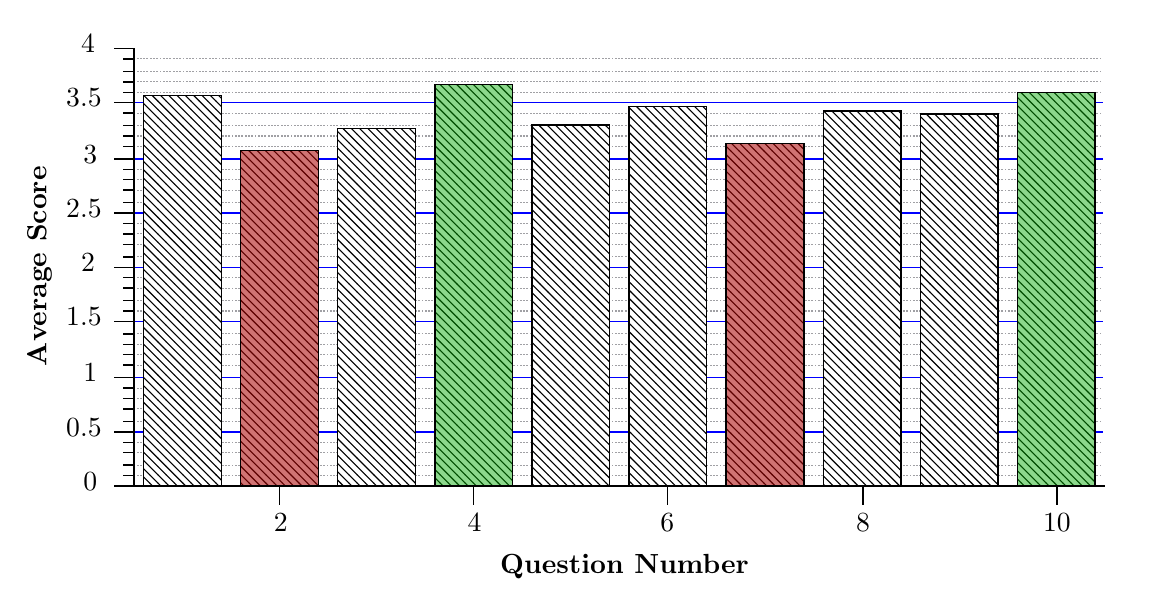
\begin{tikzpicture}{0pt}{0pt}{529pt}{265pt}
	\clip(0pt,265pt) -- (398.238pt,265pt) -- (398.238pt,65.5047pt) -- (0pt,65.5047pt) -- (0pt,265pt);
\begin{scope}
	\clip(38.3934pt,257.472pt) -- (389.204pt,257.472pt) -- (389.204pt,99.3812pt) -- (38.3934pt,99.3812pt) -- (38.3934pt,257.472pt);
	\color[rgb]{0.627451,0.627451,0.643137}
	\draw[line width=0.4pt, dash pattern=on 0.0096cm off 0.032cm, dash phase=0pt, line join=bevel, line cap=rect](38.3934pt,103.145pt) -- (388.451pt,103.145pt);
	\color[rgb]{0.627451,0.627451,0.643137}
	\draw[line width=0.4pt, dash pattern=on 0.0096cm off 0.032cm, dash phase=0pt, line join=bevel, line cap=rect](38.3934pt,106.909pt) -- (388.451pt,106.909pt);
	\draw[line width=0.4pt, dash pattern=on 0.0096cm off 0.032cm, dash phase=0pt, line join=bevel, line cap=rect](38.3934pt,111.426pt) -- (388.451pt,111.426pt);
	\draw[line width=0.4pt, dash pattern=on 0.0096cm off 0.032cm, dash phase=0pt, line join=bevel, line cap=rect](38.3934pt,115.19pt) -- (388.451pt,115.19pt);
	\draw[line width=0.4pt, dash pattern=on 0.0096cm off 0.032cm, dash phase=0pt, line join=bevel, line cap=rect](38.3934pt,122.718pt) -- (388.451pt,122.718pt);
	\draw[line width=0.4pt, dash pattern=on 0.0096cm off 0.032cm, dash phase=0pt, line join=bevel, line cap=rect](38.3934pt,127.235pt) -- (388.451pt,127.235pt);
	\draw[line width=0.4pt, dash pattern=on 0.0096cm off 0.032cm, dash phase=0pt, line join=bevel, line cap=rect](38.3934pt,130.999pt) -- (388.451pt,130.999pt);
	\draw[line width=0.4pt, dash pattern=on 0.0096cm off 0.032cm, dash phase=0pt, line join=bevel, line cap=rect](38.3934pt,134.763pt) -- (388.451pt,134.763pt);
	\draw[line width=0.4pt, dash pattern=on 0.0096cm off 0.032cm, dash phase=0pt, line join=bevel, line cap=rect](38.3934pt,143.044pt) -- (388.451pt,143.044pt);
	\draw[line width=0.4pt, dash pattern=on 0.0096cm off 0.032cm, dash phase=0pt, line join=bevel, line cap=rect](38.3934pt,146.808pt) -- (388.451pt,146.808pt);
	\draw[line width=0.4pt, dash pattern=on 0.0096cm off 0.032cm, dash phase=0pt, line join=bevel, line cap=rect](38.3934pt,150.572pt) -- (388.451pt,150.572pt);
	\draw[line width=0.4pt, dash pattern=on 0.0096cm off 0.032cm, dash phase=0pt, line join=bevel, line cap=rect](38.3934pt,154.337pt) -- (388.451pt,154.337pt);
	\draw[line width=0.4pt, dash pattern=on 0.0096cm off 0.032cm, dash phase=0pt, line join=bevel, line cap=rect](38.3934pt,162.618pt) -- (388.451pt,162.618pt);
	\draw[line width=0.4pt, dash pattern=on 0.0096cm off 0.032cm, dash phase=0pt, line join=bevel, line cap=rect](38.3934pt,166.382pt) -- (388.451pt,166.382pt);
	\draw[line width=0.4pt, dash pattern=on 0.0096cm off 0.032cm, dash phase=0pt, line join=bevel, line cap=rect](38.3934pt,170.898pt) -- (388.451pt,170.898pt);
	\draw[line width=0.4pt, dash pattern=on 0.0096cm off 0.032cm, dash phase=0pt, line join=bevel, line cap=rect](38.3934pt,174.662pt) -- (388.451pt,174.662pt);
	\draw[line width=0.4pt, dash pattern=on 0.0096cm off 0.032cm, dash phase=0pt, line join=bevel, line cap=rect](38.3934pt,182.191pt) -- (388.451pt,182.191pt);
	\draw[line width=0.4pt, dash pattern=on 0.0096cm off 0.032cm, dash phase=0pt, line join=bevel, line cap=rect](38.3934pt,186.707pt) -- (388.451pt,186.707pt);
	\draw[line width=0.4pt, dash pattern=on 0.0096cm off 0.032cm, dash phase=0pt, line join=bevel, line cap=rect](38.3934pt,190.472pt) -- (388.451pt,190.472pt);
	\draw[line width=0.4pt, dash pattern=on 0.0096cm off 0.032cm, dash phase=0pt, line join=bevel, line cap=rect](38.3934pt,194.236pt) -- (388.451pt,194.236pt);
	\draw[line width=0.4pt, dash pattern=on 0.0096cm off 0.032cm, dash phase=0pt, line join=bevel, line cap=rect](38.3934pt,201.764pt) -- (388.451pt,201.764pt);
	\draw[line width=0.4pt, dash pattern=on 0.0096cm off 0.032cm, dash phase=0pt, line join=bevel, line cap=rect](38.3934pt,206.281pt) -- (388.451pt,206.281pt);
	\draw[line width=0.4pt, dash pattern=on 0.0096cm off 0.032cm, dash phase=0pt, line join=bevel, line cap=rect](38.3934pt,210.045pt) -- (388.451pt,210.045pt);
	\draw[line width=0.4pt, dash pattern=on 0.0096cm off 0.032cm, dash phase=0pt, line join=bevel, line cap=rect](38.3934pt,213.809pt) -- (388.451pt,213.809pt);
	\draw[line width=0.4pt, dash pattern=on 0.0096cm off 0.032cm, dash phase=0pt, line join=bevel, line cap=rect](38.3934pt,222.09pt) -- (388.451pt,222.09pt);
	\draw[line width=0.4pt, dash pattern=on 0.0096cm off 0.032cm, dash phase=0pt, line join=bevel, line cap=rect](38.3934pt,225.854pt) -- (388.451pt,225.854pt);
	\draw[line width=0.4pt, dash pattern=on 0.0096cm off 0.032cm, dash phase=0pt, line join=bevel, line cap=rect](38.3934pt,229.618pt) -- (388.451pt,229.618pt);
	\draw[line width=0.4pt, dash pattern=on 0.0096cm off 0.032cm, dash phase=0pt, line join=bevel, line cap=rect](38.3934pt,234.135pt) -- (388.451pt,234.135pt);
	\draw[line width=0.4pt, dash pattern=on 0.0096cm off 0.032cm, dash phase=0pt, line join=bevel, line cap=rect](38.3934pt,241.663pt) -- (388.451pt,241.663pt);
	\draw[line width=0.4pt, dash pattern=on 0.0096cm off 0.032cm, dash phase=0pt, line join=bevel, line cap=rect](38.3934pt,245.427pt) -- (388.451pt,245.427pt);
	\draw[line width=0.4pt, dash pattern=on 0.0096cm off 0.032cm, dash phase=0pt, line join=bevel, line cap=rect](38.3934pt,249.191pt) -- (388.451pt,249.191pt);
	\draw[line width=0.4pt, dash pattern=on 0.0096cm off 0.032cm, dash phase=0pt, line join=bevel, line cap=rect](38.3934pt,253.708pt) -- (388.451pt,253.708pt);
	\color[rgb]{0,0,1}
	\draw[line width=0.5pt, line join=bevel, line cap=rect](38.3934pt,118.954pt) -- (388.451pt,118.954pt);
	\draw[line width=0.5pt, line join=bevel, line cap=rect](38.3934pt,138.528pt) -- (388.451pt,138.528pt);
	\draw[line width=0.5pt, line join=bevel, line cap=rect](38.3934pt,158.853pt) -- (388.451pt,158.853pt);
	\draw[line width=0.5pt, line join=bevel, line cap=rect](38.3934pt,178.427pt) -- (388.451pt,178.427pt);
	\draw[line width=0.5pt, line join=bevel, line cap=rect](38.3934pt,198pt) -- (388.451pt,198pt);
	\draw[line width=0.5pt, line join=bevel, line cap=rect](38.3934pt,217.573pt) -- (388.451pt,217.573pt);
	\draw[line width=0.5pt, line join=bevel, line cap=rect](38.3934pt,237.899pt) -- (388.451pt,237.899pt);
	\color[rgb]{1,1,1}
	\fill(41.9015pt,240.477pt) -- (69.9664pt,240.477pt) -- (69.9664pt,99.3812pt) -- (41.9015pt,99.3812pt) -- (41.9015pt,240.477pt);
	\color[rgb]{0,0,0}
	\draw[line width=0.5pt, line join=miter, line cap=rect](41.9015pt,240.477pt) -- (69.9664pt,240.477pt) -- (69.9664pt,99.3812pt) -- (41.9015pt,99.3812pt) -- (41.9015pt,240.477pt);
	\color[rgb]{1,1,1}
	\fill(76.9826pt,220.716pt) -- (105.047pt,220.716pt) -- (105.047pt,99.3812pt) -- (76.9826pt,99.3812pt) -- (76.9826pt,220.716pt);
	\color[rgb]{0,0,0}
	\draw[line width=0.5pt, line join=miter, line cap=rect](76.9826pt,220.716pt) -- (105.047pt,220.716pt) -- (105.047pt,99.3812pt) -- (76.9826pt,99.3812pt) -- (76.9826pt,220.716pt);
	\color[rgb]{1,1,1}
	\fill(112.064pt,228.62pt) -- (140.129pt,228.62pt) -- (140.129pt,99.3812pt) -- (112.064pt,99.3812pt) -- (112.064pt,228.62pt);
	\color[rgb]{0,0,0}
	\draw[line width=0.5pt, line join=miter, line cap=rect](112.064pt,228.62pt) -- (140.129pt,228.62pt) -- (140.129pt,99.3812pt) -- (112.064pt,99.3812pt) -- (112.064pt,228.62pt);
	\color[rgb]{1,1,1}
	\fill(147.145pt,244.429pt) -- (175.21pt,244.429pt) -- (175.21pt,99.3812pt) -- (147.145pt,99.3812pt) -- (147.145pt,244.429pt);
	\color[rgb]{0,0,0}
	\draw[line width=0.5pt, line join=miter, line cap=rect](147.145pt,244.429pt) -- (175.21pt,244.429pt) -- (175.21pt,99.3812pt) -- (147.145pt,99.3812pt) -- (147.145pt,244.429pt);
	\color[rgb]{1,1,1}
	\fill(182.226pt,229.806pt) -- (210.291pt,229.806pt) -- (210.291pt,99.3812pt) -- (182.226pt,99.3812pt) -- (182.226pt,229.806pt);
	\color[rgb]{0,0,0}
	\draw[line width=0.5pt, line join=miter, line cap=rect](182.226pt,229.806pt) -- (210.291pt,229.806pt) -- (210.291pt,99.3812pt) -- (182.226pt,99.3812pt) -- (182.226pt,229.806pt);
	\color[rgb]{1,1,1}
	\fill(217.307pt,236.525pt) -- (245.372pt,236.525pt) -- (245.372pt,99.3812pt) -- (217.307pt,99.3812pt) -- (217.307pt,236.525pt);
	\color[rgb]{0,0,0}
	\draw[line width=0.5pt, line join=miter, line cap=rect](217.307pt,236.525pt) -- (245.372pt,236.525pt) -- (245.372pt,99.3812pt) -- (217.307pt,99.3812pt) -- (217.307pt,236.525pt);
	\color[rgb]{1,1,1}
	\fill(252.388pt,223.087pt) -- (280.453pt,223.087pt) -- (280.453pt,99.3812pt) -- (252.388pt,99.3812pt) -- (252.388pt,223.087pt);
	\color[rgb]{0,0,0}
	\draw[line width=0.5pt, line join=miter, line cap=rect](252.388pt,223.087pt) -- (280.453pt,223.087pt) -- (280.453pt,99.3812pt) -- (252.388pt,99.3812pt) -- (252.388pt,223.087pt);
	\color[rgb]{1,1,1}
	\fill(287.469pt,234.944pt) -- (315.534pt,234.944pt) -- (315.534pt,99.3812pt) -- (287.469pt,99.3812pt) -- (287.469pt,234.944pt);
	\color[rgb]{0,0,0}
	\draw[line width=0.5pt, line join=miter, line cap=rect](287.469pt,234.944pt) -- (315.534pt,234.944pt) -- (315.534pt,99.3812pt) -- (287.469pt,99.3812pt) -- (287.469pt,234.944pt);
	\color[rgb]{1,1,1}
	\fill(322.55pt,233.758pt) -- (350.615pt,233.758pt) -- (350.615pt,99.3812pt) -- (322.55pt,99.3812pt) -- (322.55pt,233.758pt);
	\color[rgb]{0,0,0}
	\draw[line width=0.5pt, line join=miter, line cap=rect](322.55pt,233.758pt) -- (350.615pt,233.758pt) -- (350.615pt,99.3812pt) -- (322.55pt,99.3812pt) -- (322.55pt,233.758pt);
	\color[rgb]{1,1,1}
	\fill(357.631pt,241.663pt) -- (385.696pt,241.663pt) -- (385.696pt,99.3812pt) -- (357.631pt,99.3812pt) -- (357.631pt,241.663pt);
	\color[rgb]{0,0,0}
	\draw[line width=0.5pt, line join=miter, line cap=rect](357.631pt,241.663pt) -- (385.696pt,241.663pt) -- (385.696pt,99.3812pt) -- (357.631pt,99.3812pt) -- (357.631pt,241.663pt);
	\definecolor{c}{rgb}{0,0,0}
	\fill [pattern color=c, pattern=north west lines](41.9015pt,240.477pt) -- (69.9664pt,240.477pt) -- (69.9664pt,99.3812pt) -- (41.9015pt,99.3812pt) -- (41.9015pt,240.477pt);
	\draw[line width=0.5pt, line join=miter, line cap=rect](41.9015pt,240.477pt) -- (69.9664pt,240.477pt) -- (69.9664pt,99.3812pt) -- (41.9015pt,99.3812pt) -- (41.9015pt,240.477pt);
	\fill [pattern color=c, pattern=north west lines](76.9826pt,220.716pt) -- (105.047pt,220.716pt) -- (105.047pt,99.3812pt) -- (76.9826pt,99.3812pt) -- (76.9826pt,220.716pt);
	\draw[line width=0.5pt, line join=miter, line cap=rect](76.9826pt,220.716pt) -- (105.047pt,220.716pt) -- (105.047pt,99.3812pt) -- (76.9826pt,99.3812pt) -- (76.9826pt,220.716pt);
	\fill [pattern color=c, pattern=north west lines](112.064pt,228.62pt) -- (140.129pt,228.62pt) -- (140.129pt,99.3812pt) -- (112.064pt,99.3812pt) -- (112.064pt,228.62pt);
	\draw[line width=0.5pt, line join=miter, line cap=rect](112.064pt,228.62pt) -- (140.129pt,228.62pt) -- (140.129pt,99.3812pt) -- (112.064pt,99.3812pt) -- (112.064pt,228.62pt);
	\fill [pattern color=c, pattern=north west lines](147.145pt,244.429pt) -- (175.21pt,244.429pt) -- (175.21pt,99.3812pt) -- (147.145pt,99.3812pt) -- (147.145pt,244.429pt);
	\draw[line width=0.5pt, line join=miter, line cap=rect](147.145pt,244.429pt) -- (175.21pt,244.429pt) -- (175.21pt,99.3812pt) -- (147.145pt,99.3812pt) -- (147.145pt,244.429pt);
	\fill [pattern color=c, pattern=north west lines](182.226pt,229.806pt) -- (210.291pt,229.806pt) -- (210.291pt,99.3812pt) -- (182.226pt,99.3812pt) -- (182.226pt,229.806pt);
	\draw[line width=0.5pt, line join=miter, line cap=rect](182.226pt,229.806pt) -- (210.291pt,229.806pt) -- (210.291pt,99.3812pt) -- (182.226pt,99.3812pt) -- (182.226pt,229.806pt);
	\fill [pattern color=c, pattern=north west lines](217.307pt,236.525pt) -- (245.372pt,236.525pt) -- (245.372pt,99.3812pt) -- (217.307pt,99.3812pt) -- (217.307pt,236.525pt);
	\draw[line width=0.5pt, line join=miter, line cap=rect](217.307pt,236.525pt) -- (245.372pt,236.525pt) -- (245.372pt,99.3812pt) -- (217.307pt,99.3812pt) -- (217.307pt,236.525pt);
	\fill [pattern color=c, pattern=north west lines](252.388pt,223.087pt) -- (280.453pt,223.087pt) -- (280.453pt,99.3812pt) -- (252.388pt,99.3812pt) -- (252.388pt,223.087pt);
	\draw[line width=0.5pt, line join=miter, line cap=rect](252.388pt,223.087pt) -- (280.453pt,223.087pt) -- (280.453pt,99.3812pt) -- (252.388pt,99.3812pt) -- (252.388pt,223.087pt);
	\fill [pattern color=c, pattern=north west lines](287.469pt,234.944pt) -- (315.534pt,234.944pt) -- (315.534pt,99.3812pt) -- (287.469pt,99.3812pt) -- (287.469pt,234.944pt);
	\draw[line width=0.5pt, line join=miter, line cap=rect](287.469pt,234.944pt) -- (315.534pt,234.944pt) -- (315.534pt,99.3812pt) -- (287.469pt,99.3812pt) -- (287.469pt,234.944pt);
	\fill [pattern color=c, pattern=north west lines](322.55pt,233.758pt) -- (350.615pt,233.758pt) -- (350.615pt,99.3812pt) -- (322.55pt,99.3812pt) -- (322.55pt,233.758pt);
	\draw[line width=0.5pt, line join=miter, line cap=rect](322.55pt,233.758pt) -- (350.615pt,233.758pt) -- (350.615pt,99.3812pt) -- (322.55pt,99.3812pt) -- (322.55pt,233.758pt);
	\fill [pattern color=c, pattern=north west lines](357.631pt,241.663pt) -- (385.696pt,241.663pt) -- (385.696pt,99.3812pt) -- (357.631pt,99.3812pt) -- (357.631pt,241.663pt);
	\draw[line width=0.5pt, line join=miter, line cap=rect](357.631pt,241.663pt) -- (385.696pt,241.663pt) -- (385.696pt,99.3812pt) -- (357.631pt,99.3812pt) -- (357.631pt,241.663pt);
	\color[rgb]{0.666667,0,0}
	\fill[opacity=0.549996](41.9015pt,99.3812pt) -- (69.9664pt,99.3812pt) -- (69.9664pt,99.3812pt) -- (41.9015pt,99.3812pt) -- (41.9015pt,99.3812pt);
	\color[rgb]{0,0,0}
	\draw[line width=0.5pt, line join=miter, line cap=rect](41.9015pt,99.3812pt) -- (69.9664pt,99.3812pt) -- (69.9664pt,99.3812pt) -- (41.9015pt,99.3812pt) -- (41.9015pt,99.3812pt);
	\color[rgb]{0.666667,0,0}
	\fill[opacity=0.549996](76.9826pt,220.716pt) -- (105.047pt,220.716pt) -- (105.047pt,99.3812pt) -- (76.9826pt,99.3812pt) -- (76.9826pt,220.716pt);
	\color[rgb]{0,0,0}
	\draw[line width=0.5pt, line join=miter, line cap=rect](76.9826pt,220.716pt) -- (105.047pt,220.716pt) -- (105.047pt,99.3812pt) -- (76.9826pt,99.3812pt) -- (76.9826pt,220.716pt);
	\color[rgb]{0.666667,0,0}
	\fill[opacity=0.549996](252.388pt,223.087pt) -- (280.453pt,223.087pt) -- (280.453pt,99.3812pt) -- (252.388pt,99.3812pt) -- (252.388pt,223.087pt);
	\color[rgb]{0,0,0}
	\draw[line width=0.5pt, line join=miter, line cap=rect](252.388pt,223.087pt) -- (280.453pt,223.087pt) -- (280.453pt,99.3812pt) -- (252.388pt,99.3812pt) -- (252.388pt,223.087pt);
	\color[rgb]{0.666667,0,0}
	\fill[opacity=0.549996](357.631pt,99.3812pt) -- (385.696pt,99.3812pt) -- (385.696pt,99.3812pt) -- (357.631pt,99.3812pt) -- (357.631pt,99.3812pt);
	\color[rgb]{0,0,0}
	\draw[line width=0.5pt, line join=miter, line cap=rect](357.631pt,99.3812pt) -- (385.696pt,99.3812pt) -- (385.696pt,99.3812pt) -- (357.631pt,99.3812pt) -- (357.631pt,99.3812pt);
	\color[rgb]{0,0.666667,0}
	\fill[opacity=0.450004](41.9015pt,99.3812pt) -- (69.9664pt,99.3812pt) -- (69.9664pt,99.3812pt) -- (41.9015pt,99.3812pt) -- (41.9015pt,99.3812pt);
	\color[rgb]{0,0,0}
	\draw[line width=0.5pt, line join=miter, line cap=rect](41.9015pt,99.3812pt) -- (69.9664pt,99.3812pt) -- (69.9664pt,99.3812pt) -- (41.9015pt,99.3812pt) -- (41.9015pt,99.3812pt);
	\color[rgb]{0,0.666667,0}
	\fill[opacity=0.450004](76.9826pt,99.3812pt) -- (105.047pt,99.3812pt) -- (105.047pt,99.3812pt) -- (76.9826pt,99.3812pt) -- (76.9826pt,99.3812pt);
	\color[rgb]{0,0,0}
	\draw[line width=0.5pt, line join=miter, line cap=rect](76.9826pt,99.3812pt) -- (105.047pt,99.3812pt) -- (105.047pt,99.3812pt) -- (76.9826pt,99.3812pt) -- (76.9826pt,99.3812pt);
	\color[rgb]{0,0.666667,0}
	\fill[opacity=0.450004](147.145pt,244.429pt) -- (175.21pt,244.429pt) -- (175.21pt,99.3812pt) -- (147.145pt,99.3812pt) -- (147.145pt,244.429pt);
	\color[rgb]{0,0,0}
	\draw[line width=0.5pt, line join=miter, line cap=rect](147.145pt,244.429pt) -- (175.21pt,244.429pt) -- (175.21pt,99.3812pt) -- (147.145pt,99.3812pt) -- (147.145pt,244.429pt);
	\color[rgb]{0,0.666667,0}
	\fill[opacity=0.450004](357.631pt,241.663pt) -- (385.696pt,241.663pt) -- (385.696pt,99.3812pt) -- (357.631pt,99.3812pt) -- (357.631pt,241.663pt);
	\color[rgb]{0,0,0}
	\draw[line width=0.5pt, line join=miter, line cap=rect](357.631pt,241.663pt) -- (385.696pt,241.663pt) -- (385.696pt,99.3812pt) -- (357.631pt,99.3812pt) -- (357.631pt,241.663pt);
\end{scope}
\begin{scope}
	\color[rgb]{0,0,0}
	\pgftext[center, base, at={\pgfpoint{6.77531pt}{178.803pt}},rotate=90]{\selectfont{\textbf{Average Score}}}
	\color[rgb]{0,0,0}
	\pgftext[center, base, at={\pgfpoint{22.5844pt}{97.8756pt}}]{\selectfont{0}}
	\pgftext[center, base, at={\pgfpoint{20.3259pt}{117.449pt}}]{\selectfont{0.5}}
	\pgftext[center, base, at={\pgfpoint{22.5844pt}{137.022pt}}]{\selectfont{1}}
	\pgftext[center, base, at={\pgfpoint{20.3259pt}{157.348pt}}]{\selectfont{1.5}}
	\pgftext[center, base, at={\pgfpoint{21.8316pt}{176.921pt}}]{\selectfont{2}}
	\pgftext[center, base, at={\pgfpoint{20.3259pt}{196.494pt}}]{\selectfont{2.5}}
	\pgftext[center, base, at={\pgfpoint{22.5844pt}{216.067pt}}]{\selectfont{3}}
	\pgftext[center, base, at={\pgfpoint{20.3259pt}{236.393pt}}]{\selectfont{3.5}}
	\pgftext[center, base, at={\pgfpoint{21.8316pt}{255.966pt}}]{\selectfont{4}}
	\draw[line width=0.5pt, line join=bevel, line cap=rect](38.3934pt,103.145pt) -- (34.6294pt,103.145pt);
	\draw[line width=0.5pt, line join=bevel, line cap=rect](38.3934pt,106.909pt) -- (34.6294pt,106.909pt);
	\draw[line width=0.5pt, line join=bevel, line cap=rect](38.3934pt,111.426pt) -- (34.6294pt,111.426pt);
	\draw[line width=0.5pt, line join=bevel, line cap=rect](38.3934pt,115.19pt) -- (34.6294pt,115.19pt);
	\draw[line width=0.5pt, line join=bevel, line cap=rect](38.3934pt,122.718pt) -- (34.6294pt,122.718pt);
	\draw[line width=0.5pt, line join=bevel, line cap=rect](38.3934pt,127.235pt) -- (34.6294pt,127.235pt);
	\draw[line width=0.5pt, line join=bevel, line cap=rect](38.3934pt,130.999pt) -- (34.6294pt,130.999pt);
	\draw[line width=0.5pt, line join=bevel, line cap=rect](38.3934pt,134.763pt) -- (34.6294pt,134.763pt);
	\draw[line width=0.5pt, line join=bevel, line cap=rect](38.3934pt,143.044pt) -- (34.6294pt,143.044pt);
	\draw[line width=0.5pt, line join=bevel, line cap=rect](38.3934pt,146.808pt) -- (34.6294pt,146.808pt);
	\draw[line width=0.5pt, line join=bevel, line cap=rect](38.3934pt,150.572pt) -- (34.6294pt,150.572pt);
	\draw[line width=0.5pt, line join=bevel, line cap=rect](38.3934pt,154.337pt) -- (34.6294pt,154.337pt);
	\draw[line width=0.5pt, line join=bevel, line cap=rect](38.3934pt,162.618pt) -- (34.6294pt,162.618pt);
	\draw[line width=0.5pt, line join=bevel, line cap=rect](38.3934pt,166.382pt) -- (34.6294pt,166.382pt);
	\draw[line width=0.5pt, line join=bevel, line cap=rect](38.3934pt,170.898pt) -- (34.6294pt,170.898pt);
	\draw[line width=0.5pt, line join=bevel, line cap=rect](38.3934pt,174.662pt) -- (34.6294pt,174.662pt);
	\draw[line width=0.5pt, line join=bevel, line cap=rect](38.3934pt,182.191pt) -- (34.6294pt,182.191pt);
	\draw[line width=0.5pt, line join=bevel, line cap=rect](38.3934pt,186.707pt) -- (34.6294pt,186.707pt);
	\draw[line width=0.5pt, line join=bevel, line cap=rect](38.3934pt,190.472pt) -- (34.6294pt,190.472pt);
	\draw[line width=0.5pt, line join=bevel, line cap=rect](38.3934pt,194.236pt) -- (34.6294pt,194.236pt);
	\draw[line width=0.5pt, line join=bevel, line cap=rect](38.3934pt,201.764pt) -- (34.6294pt,201.764pt);
	\draw[line width=0.5pt, line join=bevel, line cap=rect](38.3934pt,206.281pt) -- (34.6294pt,206.281pt);
	\draw[line width=0.5pt, line join=bevel, line cap=rect](38.3934pt,210.045pt) -- (34.6294pt,210.045pt);
	\draw[line width=0.5pt, line join=bevel, line cap=rect](38.3934pt,213.809pt) -- (34.6294pt,213.809pt);
	\draw[line width=0.5pt, line join=bevel, line cap=rect](38.3934pt,222.09pt) -- (34.6294pt,222.09pt);
	\draw[line width=0.5pt, line join=bevel, line cap=rect](38.3934pt,225.854pt) -- (34.6294pt,225.854pt);
	\draw[line width=0.5pt, line join=bevel, line cap=rect](38.3934pt,229.618pt) -- (34.6294pt,229.618pt);
	\draw[line width=0.5pt, line join=bevel, line cap=rect](38.3934pt,234.135pt) -- (34.6294pt,234.135pt);
	\draw[line width=0.5pt, line join=bevel, line cap=rect](38.3934pt,241.663pt) -- (34.6294pt,241.663pt);
	\draw[line width=0.5pt, line join=bevel, line cap=rect](38.3934pt,245.427pt) -- (34.6294pt,245.427pt);
	\draw[line width=0.5pt, line join=bevel, line cap=rect](38.3934pt,249.191pt) -- (34.6294pt,249.191pt);
	\draw[line width=0.5pt, line join=bevel, line cap=rect](38.3934pt,253.708pt) -- (34.6294pt,253.708pt);
	\draw[line width=0.5pt, line join=bevel, line cap=rect](38.3934pt,99.3812pt) -- (31.6181pt,99.3812pt);
	\draw[line width=0.5pt, line join=bevel, line cap=rect](38.3934pt,118.954pt) -- (31.6181pt,118.954pt);
	\draw[line width=0.5pt, line join=bevel, line cap=rect](38.3934pt,138.528pt) -- (31.6181pt,138.528pt);
	\draw[line width=0.5pt, line join=bevel, line cap=rect](38.3934pt,158.853pt) -- (31.6181pt,158.853pt);
	\draw[line width=0.5pt, line join=bevel, line cap=rect](38.3934pt,178.427pt) -- (31.6181pt,178.427pt);
	\draw[line width=0.5pt, line join=bevel, line cap=rect](38.3934pt,198pt) -- (31.6181pt,198pt);
	\draw[line width=0.5pt, line join=bevel, line cap=rect](38.3934pt,217.573pt) -- (31.6181pt,217.573pt);
	\draw[line width=0.5pt, line join=bevel, line cap=rect](38.3934pt,237.899pt) -- (31.6181pt,237.899pt);
	\draw[line width=0.5pt, line join=bevel, line cap=rect](38.3934pt,257.472pt) -- (31.6181pt,257.472pt);
	\draw[line width=0.5pt, line join=bevel, line cap=rect](38.3934pt,257.472pt) -- (38.3934pt,99.3812pt);
	\pgftext[center, base, at={\pgfpoint{215.681pt}{67.7631pt}}]{\selectfont{\textbf{Question Number}}}
	\pgftext[center, base, at={\pgfpoint{91.4667pt}{82.8194pt}}]{\selectfont{2}}
	\pgftext[center, base, at={\pgfpoint{161.478pt}{82.8194pt}}]{\selectfont{4}}
	\pgftext[center, base, at={\pgfpoint{231.113pt}{82.8194pt}}]{\selectfont{6}}
	\pgftext[center, base, at={\pgfpoint{301.878pt}{82.8194pt}}]{\selectfont{8}}
	\pgftext[center, base, at={\pgfpoint{371.889pt}{82.8194pt}}]{\selectfont{10}}
	\draw[line width=0.5pt, line join=bevel, line cap=rect](91.0903pt,99.3812pt) -- (91.0903pt,92.6059pt);
	\draw[line width=0.5pt, line join=bevel, line cap=rect](161.102pt,99.3812pt) -- (161.102pt,92.6059pt);
	\draw[line width=0.5pt, line join=bevel, line cap=rect](231.113pt,99.3812pt) -- (231.113pt,92.6059pt);
	\draw[line width=0.5pt, line join=bevel, line cap=rect](301.878pt,99.3812pt) -- (301.878pt,92.6059pt);
	\draw[line width=0.5pt, line join=bevel, line cap=rect](371.889pt,99.3812pt) -- (371.889pt,92.6059pt);
	\draw[line width=0.5pt, line join=bevel, line cap=rect](38.3934pt,99.3812pt) -- (389.204pt,99.3812pt);
\end{scope}
\end{tikzpicture}

\caption{}\label{fig:evalGraph}
\end{figure}

The graph shows clearly that the second generation prototype scored extremely
highly in all areas. The lowest scoring questions were ``I found the system
unnecessarily complex'' and ``I would imagine that most people would learn to
use this system very quickly''. These two suggest that the appearance of the
application looks slightly too complicated to a new user and that an
improvement might be to move some of the functionality so that new users are
not overwhelmed, but that experienced users are still able to perform complex
actions.

A possible explanation for the consistently high scores is that the
participants in the questionnaire were almost all of the same age range and
were all students. Also the participants were all friends with the researchers
thus skewing their response.

\subsection{Summary of Comments}
\label{sub:summary_of_comments}

As well as the ten questions, each user was asked to comment on the good
aspects of the design, and on parts of the implementation that could be
improved.

Some of the positive comments included:
\begin{itemize}
	\item Good clean layout, nice use of colours.
	\item Clear ``Home'' screen and menus for sport location, data etc.
	\item Clear, easy to read display that allowed various ways to book a
		sporting activity.
	\item Simple flow from home screen $\rightarrow$ booking. Very few clicks
		needed to achieve desired task.
\end{itemize}

These show that the overall design of the application was clear and easy to
use, whilst still displaying all the required information, and being easy to
navigate.

From the `improvements' comments:
\begin{itemize}
	\item On ``My Bookings'', wasn't sure what sport it was.
	\item ``My Bookings'', what is temperature (is it today's temperature)?
	\item ``Select Sports'' screen, ``OK'' would have been more intuitive than
		``DONE''.
	\item Fewer sort options.
	\item The public transport section was unclear over what it meant,
		therefore i was wary to use it.
	\item The ``AM/PM'' selction in ``Time'' wasn't quite clear if I had
		selected times between selected or just selected the times.
\end{itemize}


\part{Conclusion \& Recomendations}
As with the first prototypes, the second prototype was assessed against
Neilsen’s heuristics. The application achieves a neutral or positive result
against most of the principles but needs improvement in the following areas:
\begin{itemize}
	\item error recognition, and correction,
	\item flexibility and efficiency of use.
\end{itemize}

The application was also tested against user personas and their scenarios. The
new prototype combines elements of the previous designs, which means it is
possible for the user to achieve their goal in most cases. For Joe, however, it
is likely that booking multiple courts is a rare case and would have to contact
a sports centre for information on duration and multiple court bookings.

Other possible features the application could have include additional details
such as `court surface' and something that would help the user to determine the
quality of the facilities such as a user-ratings system

The findings from the cognitive walkthroughs show that most of the steps needed
to complete a task were possible and the personas would be able to complete the
task. In some cases, the app would need the extra features mentioned above for
a user to fully achieve their goal. It also highlighted features that may be
difficult for the user to understand like the `group by' selection.

The prototype was tested by 9 people who were asked to use the prototype
system and then complete a questionnaire (see Appendix~A). The results from the
questionnaire show that, in general, the users had very few difficulties when
using the system. Some considerations that could improve the design included
simplifying the sorting and grouping options, and the repeated bookings screen
which needs to be more intuitive.

Overall, the second prototype improves the functionality of the three previous
designs but there are still features that need further development, and
functions, such as error prevention, that should be added.

\section{Recommendations}
\label{sec:recommendations}

To take this design forward we would require further prototyping to implement
the changes suggested in Section~\ref{sec:summary}.  There are a number of
additional features that we would add and several changes we would make. The
main aspects we would focus on are:

\begin{itemize}
	\item Ratings system for each location.
	\item Easier search options for booking multiple courts at once.
	\item Search options for length of booking.
	\item Notifications/reminders.
	\item Simplified sorting and grouping options.
	\item Improved error prevention.
\end{itemize}

As some of these changes are brand new features, it would be important to
prototype them before implementing them in the final design so that we could
evaluate whether they actually work in the way a user would want and expect
them to.

In addition to changing the mobile design, it could be possible to design a
similar system for the web so that users can make bookings online on a desktop
computer or laptop. This could be particularly useful for an elderly or
physically impaired user who finds a mobile phone difficult to use or a user
without a smartphone. However, this was beyond the scope of this project.

If we were to actually implement the mobile design, there are feasibility
problems which we would need to overcome. We would need to get the data for the
available sports at each location and the data for the individual booking slots
at each location and whether the booking slots were already booked or not. This
would be possible through two methods:

\begin{enumerate}
	\item Direct involvement of the sports facilities. They would provide the
		data directly to us and would allow a connection to their own systems
		in order to actually make, cancel and change the bookings.

	\item Scraping the data from the websites of each facilities, or get access
		to the data through APIs provided by these websites. In order to make a
		booking, the user would be redirected to the website of that particular
		facility.
\end{enumerate}

The first option is preferable as it would allow the user to make and amend
bookings directly through the application. The prototypes that we have made in
this project would require the involvement of the sports facilities. If, going
forward, this were to be revealed as unfeasible, we could possibly use the
second method above. This would require a lot of changes in the design and
therefore numerous more prototypes.

\section{Summary}
\label{sec:summary}

Our aim was to design a mobile booking system for sports centres that would
allow users to search multiple facilities at the same time and compare results.
This is something that can be done with many booking applications for other
services.

Through our research into mobile booking apps and sports facilities websites,
we identified key design features for our application. We also found that the
interface may have to present a large amount of data. Readability and filtering
results would have to be considered as well as an easy-to-use, clean interface.
We then used these findings to design our first generation prototypes. These
were based on the three navigation styles outlined by Apple Inc; hierarchical,
flat, and content-driven.

We evaluated the first generation prototypes using Nielsen’s heuristics and
user personas. We found that each design had features that were useful and
satisfied specific scenarios. These were then incorporated into the design of
the second prototype.

The second prototype was able to achieve more than the previous designs but the
cognitive walkthroughs and questionnaire results show there are some areas that
would need further development if this application were to be taken forward.

\subsection{Next Steps}
\label{sub:next_steps}

% TODO

\subsection{Team Analysis}
\label{sub:team_analysis}

Our approach to the project was well structured in that we researched related
existing systems and work that addresses similar principles and techniques,
this helped us better prepare when designing our system. We were also very
cautious in assuming to understand the user which can be a common mistake to
make being the designer of the system. The user personas and scenarios were
created to avoid this problem. We ensured that we used a variety of inspection
and empirical evaluation methods on our final design to expose any issues which
users may face when interacting with the interface.  In terms of changing and
improving our approach we could have spent more time incorporating other
features such as showing the rating and have the user request a notification
nearer to the time of their booking. The lack of such features came up in our
evaluation but were discarded from the final design. We could have increased
the reliability and validity of our SUS results by having more participants
from a more varied and wider demographic.

As a group, we met weekly and worked well in distributing our work fairly and
evenly. Each week we each had our own task and every member of the group worked
hard to meet the deadlines. Our work was kept well organized on Google Drive so
any member of the group could view and make changes on all the documents
created.


\vfill
\part{Appendix}

\appendix
\addcontentsline{toc}{section}{A\hspace{3pt} SUS Questionnaire}
\includepdf{../EvaluationQuestionnaire/build/EvaluationQuestionnaire.pdf}
\stepcounter{section}
\section{Questionnaire Results}
\label{app:questionnaire_results}

The list of individual results from the SUS questionnaire is shown below.
% \renewcommand{\arraystretch}{1.3}
% \begin{longtabu}{rlrlrlrl}
% 	\toprule
% 	Score & Percentage &&&&&&\\
% 	\midrule
% 32 & 80.0 &  & 36 & 90.0 &  & 31   & 77.5 \\
% 32 & 80.0 &  & 37 & 92.5 &  & 35   & 87.5 \\
% 33 & 82.5 &  & 29 & 72.5 &  & 35   & 87.5 \\
% 39 & 97.5 &  & 31 & 77.5 &  & 32   & 80.0 \\
% 34 & 85.0 &  & 26 & 65.0 &  & 37   & 92.5 \\
% 36 & 90.0 &  & 33 & 82.5 &  & 38   & 95.0 \\
% 33 & 82.5 &  & 32 & 80.0 &  & 37   & 92.5 \\
% 32 & 80.0 &  & 33 & 82.5 &  & 39   & 97.5 \\
% 33 & 82.5 &  & 32 & 80.0 &  & 32   & 80.0 \\
% 38 & 95.0 &  & 38 & 95.0 &  & 32   & 80.0 \\ \midrule
% \multicolumn{2}{l}{Average}      &  &    &      &  & 34.2 & 85.5\% \\
% 	\bottomrule
% \end{longtabu}

\renewcommand{\arraystretch}{1.3}
\begin{longtabu}{rrl}
	\toprule
	& Score & Percentage \\
	\midrule
& 32 & 80.0 \\
& 32 & 80.0 \\
& 33 & 82.5 \\
& 39 & 97.5 \\
& 34 & 85.0 \\
& 36 & 90.0 \\
& 33 & 82.5 \\
& 32 & 80.0 \\
& 33 & 82.5 \\
& 38 & 95.0 \\ \midrule
Average & 34.2 & 85.5\% \\
	\bottomrule
\end{longtabu}

\section{Project Log}
\label{sec:project_log}

\renewcommand{\arraystretch}{1.3}
\begin{longtabu}{llCccX}
\toprule
Date       & Time & Length & Room & Appologies & Plan                                                                                        \\
           &      & (hours)&      &            &                                                                                             \\
\midrule
17/01 & 1100 & 1 & UG04 & N & Brainstorm project possibilites                                                                                 \\
23/01 & 1400 & 1 & UG04 & N & Finalise draft proposal. Discuss review of related work + decide who is researching which section               \\
31/01 & 1100 & 2 & UG04 & N & Finalise review of related work. Discuss analysis of user requirements + decide who is researching each section \\
07/02 & 1100 & 2 & UG04 & N & Finalise personas and discuss prototypes                                                                        \\
14/02 & 1100 & 2 & UG04 & N & Finalise first prototypes and discuss second prototype                                                          \\
21/02 & 1100 & 2 & UG04 & N & Discuss progress on second prototype                                                                            \\
28/02 & 1200 & 1 & UG04 & N & Finalise second prototype and discuss evaluation results                                                        \\
07/03 & 1100 & 1 & UG04 & N & Discuss summary and anaylsis of project                                                                         \\
11/03 & 1400 & 1 & UG04 & N & Review report, everyone to read through and check for errors.                                                   \\
\bottomrule
\end{longtabu}


\bibliographystyle{unsrt}
\bibliography{references}

\end{document}

% vim: autochdir
